% Este documento destina-se a servir como modelo para a produção de documentos
% de pesquisa do PPGINF/UFPR, como projetos, dissertações e teses. A classe de
% documento se chama "ppginf" (arquivo ppginf.cls) e define o formato básico do
% documento. O texto está organizado em capítulos que são colocados em
% subdiretórios separados. São definidos exemplos para a inclusão de figuras,
% códigos-fonte e a definição de tabelas.
%
% Produzido por Carlos Maziero (maziero@inf.ufpr.br) em Outubro de 2015.
% Baseado em um modelo anterior construído pelo autor para o PPGIA/PUCPR.

% Opções da classe ppginf:
%
% - defesa  : versão para entregar à banca; tem espaçamento 1,5
%             e omite algumas páginas iniciais (agradecimentos, etc)
% - final   : versão pós-defesa, para enviar à biblioteca;
%             tem espaçamento simples e todas as páginas iniciais.
% - oneside : somente frente; use quando for gerar somente o PDF.
% - twoside : frente/verso; use quando for gerar uma versão impressa.
% - ...     : demais opções aceitas pela classe "book"

% Sobre línguas: o modelo tem suporte para português e inglês. As duas 
% línguas devem ser informadas como opção da classe; a língua principal
% do documento deve vir POR ÚLTIMO.

% Opções default: defesa, oneside, texto principal em português
\documentclass[defesa,oneside,english,brazilian]{ppginf}	% defesa
%\documentclass[defesa,oneside,brazilian,english]{ppginf}	% defesa, inglês
%\documentclass[final,oneside,english,brazilian]{ppginf}	% final PDF
%\documentclass[final,twoside,english,brazilian]{ppginf}	% final impressa

% configurações de diversos pacotes, inclusive o fonte principal do texto
% Pacotes usados neste documento e suas respectivas configurações

% ------------------------------------------------------------------------------

% Definição de fontes

% formato dos arquivos-fonte (utf8 no Linux e latin1 no Windows)
\usepackage[utf8]{inputenc}	% arquivos LaTeX em Unicode (UTF8)

% usar codificação T1 para ter caracteres acentuados corretos no PDF
\usepackage[T1]{fontenc}

% fonte usada no corpo do texto (descomente apenas uma)
\usepackage{newtxtext,newtxmath}	% Times (se não tiver, use mathptmx)
%\usepackage{lmodern}			% Computer Modern (fonte clássico LaTeX)
%\usepackage{kpfonts}			% Kepler/Palatino (idem, use mathpazo)
%\renewcommand{\familydefault}{\sfdefault} % Arial/Helvética (leia abaixo)

% A biblioteca central da UFPR recomenda usar Arial, seguindo a recomendação da
% ABNT. Essa é uma escolha ruim, pois fontes sans-serif são geralmente inade-
% quados para textos longos e impressos, sendo melhores para páginas Web.
% http://www.webdesignerdepot.com/2013/03/serif-vs-sans-the-final-battle/.

% fontes usadas em ambientes específicos
\usepackage[scaled=0.9]{helvet}		% Sans Serif
\usepackage{courier}			% Verbatim, Listings, etc

% ------------------------------------------------------------------------------

% inclusão de figuras em PDF, PNG, PS, EPS
\usepackage{graphicx}

% subfiguras (subfigure is deprecated, don't use it)
\usepackage[labelformat=simple]{subcaption}
\renewcommand\thesubfigure{(\alph{subfigure})}

% ------------------------------------------------------------------------------

% inclusão/formatação de código-fonte (programas)
\usepackage{listings}
\lstset{language=c}
\lstset{basicstyle=\ttfamily\footnotesize,commentstyle=\textit,stringstyle=\ttfamily}
\lstset{showspaces=false,showtabs=false,showstringspaces=false}
\lstset{numbers=left,stepnumber=1,numberstyle=\tiny}
\lstset{columns=flexible,mathescape=true}
\lstset{frame=single}
\lstset{inputencoding=utf8,extendedchars=true}
\lstset{literate={á}{{\'a}}1  {ã}{{\~a}}1 {à}{{\`a}}1 {â}{{\^a}}1
                 {Á}{{\'A}}1  {Ã}{{\~A}}1 {À}{{\`A}}1 {Â}{{\^A}}1
                 {é}{{\'e}}1  {ê}{{\^e}}1 {É}{{\'E}}1  {Ê}{{\^E}}1
                 {í}{{\'\i}}1 {Í}{{\'I}}1
                 {ó}{{\'o}}1  {õ}{{\~o}}1 {ô}{{\^o}}1
                 {Ó}{{\'O}}1  {Õ}{{\~O}}1 {Ô}{{\^O}}1
                 {ú}{{\'u}}1  {Ú}{{\'U}}1
                 {ç}{{\c{c}}}1 {Ç}{{\c{C}}}1 }

% ------------------------------------------------------------------------------

% formatação de algoritmos
\usepackage{algorithm,algorithmic}
\iflanguage{brazilian} {\floatname{algorithm}{Algoritmo}}{}
\renewcommand{\algorithmiccomment}[1]{~~~// #1}
%\algsetup{linenosize=\footnotesize,linenodelimiter=.}

% ------------------------------------------------------------------------------

% listas de símbolos e de abreviações (a fazer)
%\usepackage[titles]{tocloft}
%\newlistof[part]{symb}{los}{Lista de Símbolos}
%\newlistof[part]{abbrev}{loa}{Lista de Abreviações}
%\newcommand{\symb}[2]{%
%\refstepcounter{symb}
%\addcontentsline{los}{symb}{\protect #1 :#2}\par}

% ------------------------------------------------------------------------------

% formatação de bibliografia
\usepackage{natbib}		% bibliografia no estilo NatBib

% EXIGÊNCIA DA BIB@UFPR
% muda o título das referências em português para "Referências"
\addto{\captionsbrazilian}{\renewcommand{\bibname}{Refer\^encias}}
\addto{\captionsenglish}{\renewcommand{\bibname}{References}}

% ------------------------------------------------------------------------------

% outros pacotes diversos
\usepackage{alltt,moreverb}	% mais comandos no modo verbatim
\usepackage{lipsum}		% gera texto aleatório (para os exemplos)
\usepackage{currfile}		% infos sobre o arquivo/diretório atual
\usepackage[final]{pdfpages}	% inclusão de páginas em PDF
\usepackage{longtable}		% tabelas multi-páginas (tab símbolos/acrônimos)

% ------------------------------------------------------------------------------



%=====================================================

\begin {document}

% Principais dados, usados para gerar as páginas iniciais.
% Campos não utilizados podem ser removidos ou comentados.

% título
\title{Um modelo \LaTeX\ para dissertações e teses \\ (escrevi um título mais longo para ver como se comporta a quebra de linhas e o espaçamento entre elas)}

% palavras-chave e keywords (p/ resumo, abstract e metadados do PDF)
\pchave{palavra-chave 1, palavra-chave 2, palavra-chave 3}
\keyword{keyword 1, keyword 2, keyword 3}

% autoria
\author{Felipe Amorim e Murilo Vidal}
\advisor{Donald Knuth}
\coadvisor{Leslie Lamport}

% instituição
\iflanguage{brazilian}
  { \instit{UFPR}{Universidade Federal do Paraná} }
  { \instit{UFPR}{Federal University of Paraná} }

% área de concentração (default do PPGInf, não mudar)
\iflanguage{brazilian}
  { \field{Ciência da Computação} }
  { \field{Computer Science} }

% data (só o ano)
\date{2018}

% local
\iflanguage{brazilian}
  { \local{Curitiba PR} }
  { \local{Curitiba PR - Brazil} }

% imagem de fundo da capa (se não desejar, basta comentar)
\coverimage{0-iniciais/fundo-capa.jpg}

%=====================================================

%% Descrição do documento (obviamente, descomentar somente UMA!)

\iflanguage{brazilian}
{
% tese de doutorado
\descr{Tese apresentada como requisito parcial à obtenção do grau de Doutor em Ciência da Computação no Programa de Pós-Graduação em Informática, Setor de Ciências Exatas, da Universidade Federal do Paraná}

% exame de qualificação de doutorado
%\descr{Documento apresentado como requisito parcial ao exame de qualificação de Doutorado no Programa de Pós-Graduação em Informática, Setor de Ciências Exatas, da Universidade Federal do Paraná}

% dissertação de mestrado
%\descr{Dissertação apresentada como requisito parcial à obtenção do grau de Mestre em Informática no Programa de Pós-Graduação em Informática, Setor de Ciências Exatas, da Universidade Federal do Paraná}

% exame de qualificação de mestrado
%\descr{Documento apresentado como requisito parcial ao exame de qualificação de Mestrado no Programa de Pós-Graduação em Informática, Setor de Ciências Exatas, da Universidade Federal do Paraná}

% trabalho de conclusão de curso
%\descr{Trabalho apresentado como requisito parcial à conclusão do Curso de Bacharelado em XYZ, Setor de Ciências Exatas, da Universidade Federal do Paraná}

% trabalho de disciplina
%\descr{Trabalho apresentado como requisito parcial à conclusão da disciplina XYZ no Curso de Bacharelado em XYZ, Setor de Ciências Exatas, da Universidade Federal do Paraná}
}
{
% doctorate thesis
\descr{Thesis presented as a partial requirement for the degree of Doctor in Computer Science in the Graduate Program in Informatics, Exact Sciences Sector, of the Federal University of Paraná, Brazil}

% doctorate qualification
%\descr{Document presented as a partial requirement for the doctoral qualification exam in the Graduate Program in Informatics, Exact Sciences Sector, of the Federal University of Paraná, Brazil}

% MSc dissertation
%\descr{Dissertation presented as partial a requirement for the degree of Master of Sciences in Informatics in the Graduate Program in Informatics, Exact Sciences Sector, of the Federal University of Paraná, Brazil.}

% MSc qualification
%\descr{Document presented as a partial requirement for the Master of Sciences qualification exam in the Graduate Program in Informatics, Exact Sciences Sector, of the Federal University of Paraná, Brazil}

% trabalho de conclusão de curso, inglês
%\descr{to be translated}

% trabalho de disciplina, inglês
%\descr{to be translated}
}

%=====================================================

% define estilo das páginas iniciais (capas, resumo, sumário, etc)
\frontmatter
\pagestyle{frontmatter}

% define capa e folha de rosto
\titlepage

% páginas que só aparecem na versão final (a inclusão é automática)
% - IMPORTANTE - IMPORTANTE - IMPORTANTE - IMPORTANTE -
%
% O conteúdo exato da ficha catalográfica é preparada pela Biblioteca Central
% da UFPR, a pedido da secretaria do PPGINF. Não "invente" um conteúdo para ela,
% se informe a respeito com a secretaria do programa.

\begin{ficha}	% só gera conteúdo se for na versão final

% inclusão da ficha catalográfica final (arquivo PDF)
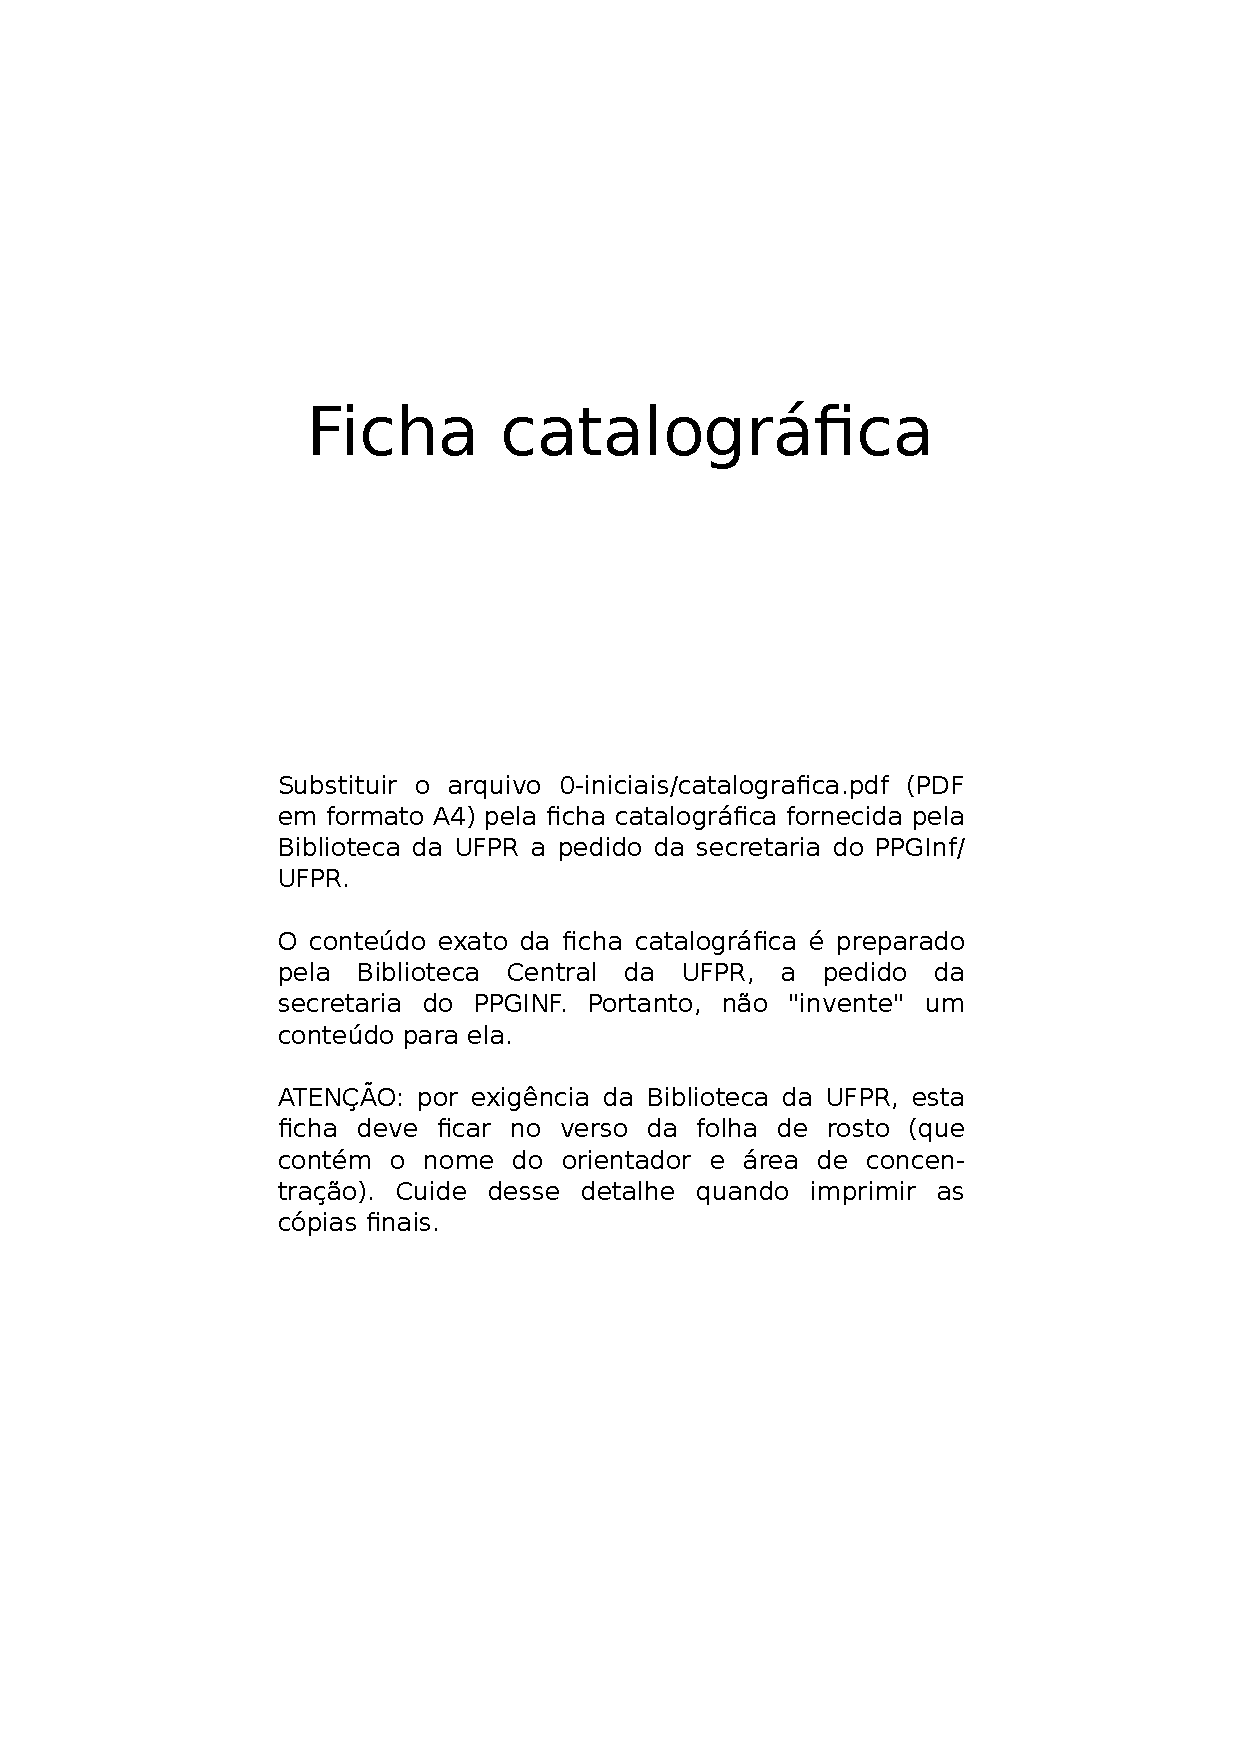
\includepdf[noautoscale]{0-iniciais/catalografica.pdf}

\end{ficha}

%=====================================================
	% ficha catalográfica
% A ficha de aprovação será fornecida pela secretaria do programa,
% após a defesa e cumprimento dos demais trâmites legais.

\begin{aprovacao}	% só gera conteúdo se for na versão final

% inclusão do termo de aprovação final (arquivo PDF)
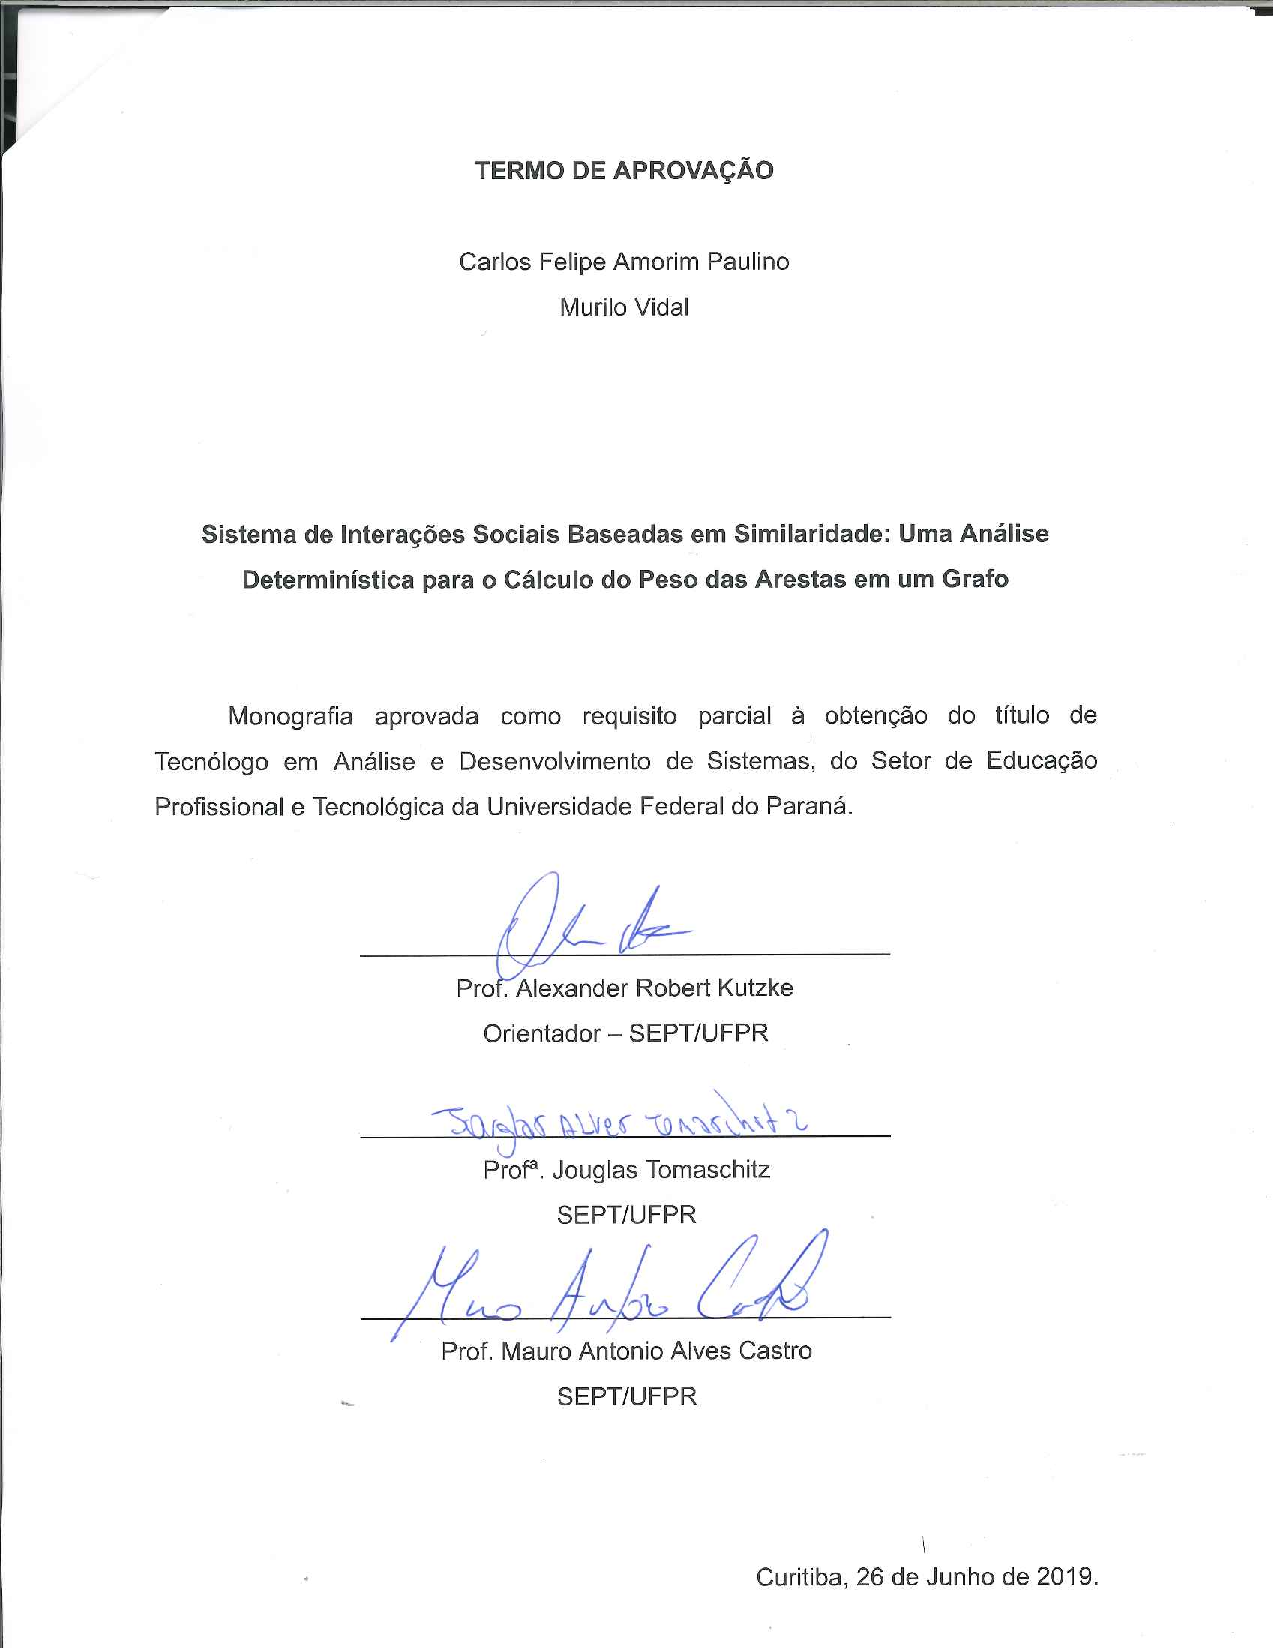
\includepdf[noautoscale]{0-iniciais/aprovacao.pdf}

\end{aprovacao}

%=====================================================
		% folha de aprovação
\begin{dedica}  % só gera conteúdo se for na versão final

A alguém...

\end{dedica}

		% dedicatória
\begin{agradece}	% só gera conteúdo se for na versão final

Somos muitíssimo gratos a nossos pais, Josefa e José, e Clarice e Adriano, pelo apoio e carinho. Um particular agradecimento às nossas companheiras, Fernanda e Bruna, pela paciência, compreensão e, sempre disponível, atenção. Vocês foram essenciais em todos os momentos do desenvolvimento deste trabalho. Obrigado, Julia, pela disponibilidade e amizade, seu talento deu cores ao nosso sistema.

Ao professor Alex, nossos sinceros agradecimentos pela orientação, conhecimento compartilhado, incentivo e bons sentimentos. Ao professor Jouglas e ao professor Mauro, por comporem a banca de avaliação e nos iluminarem com bons comentários e críticas, nosso reconhecimento e gratidão.



\end{agradece}

		% agradecimentos

% resumo (português) e abstract (inglês)
\begin{resumo}
\singlespacing
\noindent
As relações sociais são cada vez mais realizadas em ambiente virtual, o que traz a possibilidade de encontrar pessoas de várias culturas e com diferentes opiniões. Porém, por vezes o usuário da rede social quer apenas encontrar seus pares e compartilhar interesses mútuos. Este trabalho visa construir uma rede social com foco em sugestão de novos relacionamentos baseados em interesses mútuos, sem priorizar a aparência do usuário. Nesta rede, os usuários podem relacionar-se anonimamente por uma dinâmica de perguntas e respostas, na qual é possível compartilhar questões, responder perguntas dos outros usuários e avaliar as respostas recebidas. Conforme a interação nesse modelo vai acontecendo, o sistema convida os contatos considerados similares para relacionarem-se mais proximamente pelo uso de um mensageiro instantâneo particular. Dessa maneira, os usuários entram em contato com pessoas novas tendo sido mensurada a similaridade entre cada usuário com base em um cálculo determinístico. A rede social tratada neste trabalho é representada por um grafo no qual os nós são os usuários, as arestas são as conexões entre eles e o peso das arestas determina o grau de similaridade entre os usuários. Este método de sugestão de contatos tem a ambição de ser eficaz, de maneira que demande pouca carga de processamento, pois, é uma função do número de respostas recebidas e avaliadas. Ao longo do desenvolvimento do software o cálculo do peso da aresta foi testado com várias equações e os resultados foram comparados  entre si. Uma equação foi selecionada como a mais adequada e os resultados foram considerados satisfatórios. O cálculo do valor do peso da aresta do grafo é eficiente e leve; o produto final é atrativo e a dinâmica de perguntas e respostas tem a possibilidade de direcionar o usuário para relacionamentos que tratem de assuntos que lhe interessem naturalmente. Outras possibilidades de pesquisas futuras foram iluminadas com este trabalho de maneira que surgiram novas ideias de incremento na sofisticação do cálculo do peso das arestas do grafo, seja pelo emprego de inteligência artificial ou pela mineração de dados provenientes das interações por meio da análise semântica dos textos compartilhados entre os usuários.

\end{resumo}

\begin{abstract}
\singlespacing
\noindent
The social relationships are increasingly taking place in the virtual environment, which brings the possibility of meeting people of various cultures and with divergent opinions. However, sometimes the user of the social media wishes only to meet his peers and share common interests. This work seeks to build a social media focused in suggesting new relationships based in common interests, without prioritizing the looks of the user. In this network, the users can relate anonymously by a dynamic of questions and answers, in which is possible to share questions, answer another users’ questions and evaluate the received answers. As the interaction in this model is happening, the system invites the contacts considered similar to relate closely by the use of a private instant messenger. That way, the users get in touch with new people as the similarity between each user is measured based in a deterministic calculation. The social media subject of this work is represented by a graph in which the nodes are the users, the edges are the connexion between them and the weight of the edges determines the grade of similarity between the users. This method of contacts suggestion has the ambition of being efficient, in a way that it demands little processing power as it is simply a function of the number of answers received and evaluated. Throughout the software development the edge weight calculation was tested with several equations and the results were compared to each other. An equation was selected as the most suitable and the results were considered satisfactory. The edge weight calculation is lightweight and efficient; the final product is attractive and the dynamic of questions and answers has the possibility of directing the user to relationships that  deal with subjects that interest them naturally. Another possibilities of further research were unveiled with this work as new ideas to increase the sophistication of the graph’s edge’s weight calculation, be it by employing artificial intelligence or by mining data from the interactions thru the semantic analysis of the texts shared between the users.

\end{abstract}


% listas  de figuras, tabelas, abreviações/siglas, símbolos
\listoffigures
\clearpage
\listoftables
%=====================================================

% lista de acrônimos (siglas e abreviações)

\begin{listaacron}

\begin{longtable}[l]{p{0.2\linewidth}p{0.7\linewidth}}
TADS & Tecnologia em Análise e Desenvolvimento de Sistemas\\
SDK & \emph{Software development kit}\\
VM & \emph{Virtual Machine}\\
UFPR & Universidade Federal do Paraná\\
\end{longtable}

\end{listaacron}

%=====================================================
		% ainda deve ser preenchida à mão
%=====================================================

% lista de símbolos

\begin{listasimb}

\begin{longtable}[l]{p{0.2\linewidth}p{0.7\linewidth}}
$\alpha$ & alfa, primeira letra do alfabeto grego\\
$\beta$ & beta, segunda letra do alfabeto grego\\
$\gamma$ & gama, terceira letra do alfabeto grego\\
$\omega$ & ômega, última letra do alfabeto grego\\
$\pi$ & pi \\
$\tau$ & Tempo de resposta do sistema\\
$\theta$ & Ângulo de incidência do raio luminoso\\
\end{longtable}

\end{listasimb}

%=====================================================
		% idem

% sumário
\tableofcontents

%=====================================================

% define estilo do corpo do documento (capítulos e apêndices)
\mainmatter
\pagestyle{mainmatter}

% inclusao de cada capítulo, alterar a gosto (do professor de Metodologia)
\chapter{Fundamentação Teórica}
\label{cap:fund}

% figuras estão no subdiretório "figuras/" dentro deste capítulo
\graphicspath{\currfiledir/figuras/}

Nesta parte, há a exposição das definições e histórico de redes sociais, algoritmos de recomendação e as definições matemáticas e computacionais de grafo. Esses três itens relacionam-se intrinsicamente com este trabalho, por isso, buscamos esclarecê-los o suficiente neste capítulo de maneira que as relações destes tópicos com o objetivo geral estejam fundamentadas.


\section{Redes Sociais}

% \begin{itemize}
% \item Histórico de redes sociais
% \item Tipos de redes sociais
% \item Redes parecidas com nosso trabalho
% \item Análises de tempo despendido em redes sociais.
% \end{itemize}

Desde a invenção da internet em 1991, mais e mais aplicações vem sendo criadas para facilitar e estimular os relacionamentos virtuais. As redes sociais virtuais tiveram início em 1997 com o site \emph{Six Degrees}, \citep{terrel17}. \emph{Six Degrees} é nomeado em referência ao estudo de \cite{milgram67}, que teorizava que são necessários seis laços de amizade para que quaisquer pessoas estejam conectadas. \emph{Six Degrees} teve seu fim em 2001, mas iniciou o processo de popularização das redes sociais e é considerado a primeira rede social pois permitia que as pessoas criassem seus perfis individuais e adicionar outros contatos à sua rede. Teve 3,5 milhões de usuários no seu auge.

Entre as precursoras está também a rede especializada em relacionamentos profissionais, \emph{LinkedIn}. Foi criada no final de 2002 e tem, desde então, seu objetivo principal em criar conexões entre profissionais, estudantes e corporações. O \emph{LinkedIn} é, ainda hoje, a rede mais popular neste nicho com mais de 500 milhões de usuários.

A rede mais popular atualmente, segundo \cite{lua19}, é o Facebook com 2,23 milhões de usuários ativos mensalmente. O Facebook foi criado em 2004 como uma rede específica para estudantes da Universidade de Harvard. Em 2006 foi aberta ao público e em 2008 já era a rede social mais visitada do mundo.

Há também redes especializadas em outros tipos de conexão ou outras maneiras de publicar conteúdo. O YouTube é uma rede social especializada na divulgação de vídeos criados pelos usuários. O Twitter, distingue-se das outras redes por iniciar suas atividades permitindo apenas a publicação de textos com, no máximo, 140 caracteres. Este limite foi dobrado posteriormente, mas o foco ainda mantém-se em pequenas postagens.

Por fim, há as redes especializadas em relacionamentos românticos. O Tinder, o Happn e o OKCupid são exemplos de redes sociais direcionadas à criação de relacionamentos íntimos entre os usuários. O sistema desenvolvido neste trabalho enquadra-se nesta categoria pois tem o objetivo de colocar usuários em contato com pessoas desconhecidas que têm potencial para formarem amizades ou até mesmo casais.

No Brasil, 66\% da população tem acesso à internet segundo \cite{wearesocial18}. Dentre os usuários da internet 93\% são ativos em alguma rede social.
Segundo \cite{wearesocial18}, o brasileiro despende, em média, 3h39min por dia em alguma rede social. Este tempo é passado em contato com informações e pessoas de várias culturas diferentes. Muitas vezes as interações despertam sentimentos indesejados e a informação divulgada não é completamente conexa à realidade.

Por essa razão, mais e mais redes sociais oferecem a oportunidade, muitas vezes compulsoriamente, do usuário ser exposto somente à pessoas e conteúdos que tenham afinidade com seu perfil. Na busca por uma experiência agradável, as sugestões de conteúdo e contatos vão ao encontro da necessidade do ser humano de se socializar. E participar de uma rede social, seja ela física ou virtual, faz parte das necessidades básicas apontadas por \cite{Maslow1943}, ao definir uma hierarquia para as necessidades básicas do ser humano.

De uma maneira ou de outra, todas as redes sociais tem seu foco no conteúdo gerado pelos usuários. Porém, grande parte da monetização empregada refere-se à divulgação de peças publicitárias pagas por empresas particulares e públicas. Dentro deste escopo, são utilizados algoritmos que tomam em conta os interesses dos usuários para fazer sugestões de conteúdo publicitário. Há vários métodos para relacionar os dados produzidos pelos usuários para gerar sugestões, sejam elas de conteúdo, publicidade ou novos contatos.

%=====================================================

\section{Algoritmos de Recomendação}

% \begin{itemize}
% \item Como sugerir novos contatos.
% \item Como as outras redes fazem isso.
% 
% \end{itemize}


Quando um usuário acessa um sistema qualquer que lhe oferece itens, por exemplo, livros, um sistema de recomendação pode lhe proporcionar a conveniência de sugerir-lhe um livro mais adequado para o seu gosto quando a quantidade de opções disponíveis é opressivamente vasta, diz \cite{Ricci2010}.

Esses itens, são quaisquer coisas que podem ser sugeridas ao usuário, sejam produtos, serviços, notícias, publicidade, ou, no caso deste trabalho, outros usuários com potencial para tornarem-se amizades.

Para \cite{Ricci2010}, a forma mais simples de um sistema de recomendação é uma lista com itens ordenados pela similaridade com o usuário que receberá a recomendação. Os sistemas de sugestão analisam vários tipos de dados por diversos métodos diferentes para encontrar os itens mais adequados para cada usuário. De acordo com \cite{Ricci2010}, os primeiros algoritmos de recomendação utilizavam dados gerados por recomendações feitas pela comunidade de usuários. Esse método comparava gostos similares entre os usuários e recomendava itens ainda não consumidos por alguns usuários. A este método dá-se o nome de Filtragem Colaborativa \citep{goldberg92}.

Desde os anos 1990, a perseguição por sistemas de recomendações cada vez mais eficientes impulsionou o surgimento do Prêmio Netflix em 2006, \citep{netflix}. Neste concurso, a empresa Netflix propôs pagar um prêmio de US\$1.000.000 para quem elaborasse um sistema que pudesse melhorar em, pelo menos, 10\% a acurácia do sistema que estava em uso à época. O time \emph{BellKor's Pragmatic Chaos}, venceu a disputa empregando diversos algoritmos e métodos de classificação mesclados em um mesmo sistema, \citep{Bell}. 

Entre as possibilidades de métodos e algoritmos que podem ser empregados em um sistema de recomendação, podemos ressaltar, baseados no texto de \cite{Recommendation}, as seguintes:

\begin{itemize}
\item Filtragem colaborativa
\item Filtragem baseada em conteúdo
\item Recomendação baseada em conhecimento
\end{itemize}

A filtragem colaborativa, como já mencionado, leva em conta as preferências já informadas pelos usuários para compará-las e sugerir novas possibilidades de itens. Tem a tendência de sugerir itens que já são apreciados por usuários que, de alguma maneira, já se relacionam, seja por interesses definidos, grupos específicos ou até mesmo por parentesco.

A filtragem baseada em conteúdo toma por verdadeira a afirmação de que os usuários que já demonstraram interesse por um tópico somente serão agradados por tópicos semelhantes e não podem ser instigados por assuntos fora do escopo do que já foi definido como interesse inicialmente. Dessa maneira, o sistema considera de que um usuário que declarou interesse por filmes deve receber sugestões de itens relacionados a este tema. É claro que este método tem a fraqueza de não sugerir novos assuntos que, potencialmente, despertariam o interesse do usuário.

Finalmente, a recomendação baseada em conhecimento,  que toma em conta regras de restrições de interesse definidas no sistema e os aplica à lista de itens disponíveis. Desse modo, os itens são sugeridos a partir do resultado da filtragem realizada a partir das regras definidas. A definição de tais regras passa por análises semânticas do conteúdo disponível no sistema que diga respeito ao usuário. O sistema desenvolvido neste trabalho assemelha-se a uma recomendação baseada em conhecimento no sentido de que a regra definida para relacionar os itens será uma equação determinística que calcula um valor de proximidade entre dois itens.

Os vários métodos de recomendação tem sua acurácia diretamente influenciada pela quantidade de informação disponível sobre os usuários ou gerada pelos usuários. Quanto maior a quantidade de informação disponível, maior a acurácia e, em linhas gerais, menor a performance do sistema, uma vez que o tempo de processamento da informação é incrementado. Por essa razão, boas soluções são baseadas em aprendizado de máquina e inteligência artificial. O emprego dessas tecnologias tem o objetivo de melhorar a performance e a acurácia das sugestões.

%=====================================================

\section{Grafo}
% \begin{itemize}
% \item O que é grafo - \emph{Fonte básica de definição de grafo LIVRO??}
% \item Quantos tipos de grafo existem.
% \item Aplicações comuns de grafo
% \item Algoritmos que usam grafos
% \end{itemize}

O conceito matemático de grafo parte de abstrações de situações da vida real onde objetos ou pessoas representadas por pontos e suas conexões e interações são representadas por linhas \cite{Bondy08}. Numa rede social, as pessoas são esses pontos, que convencionalmente são chamados de nós, e suas relações com outras pessoas são representadas por linhas, chamadas de arestas. Um grafo é uma tripla ordenada $G=(N(G), A(G), \psi _{G})$, que consiste de um conjunto não vazio $N(G)$ de nós, um conjunto $A(G)$, diferente de $N(G)$, de arestas, e uma \emph{função de incidência} $\psi_{G}$ que associa a cada nó de $G$ um par não ordenado de nós de $G$. Se $e$ é uma aresta de $G$ e $u$ e $v$ são arestas de tal modo que $\psi_{G}(e) = un$, então $e$ é dito que \emph{une} $u$ e $n$ \cite{Bondy08}.

\emph{Exemplo}

\begin{equation}
G=(N(G), A(G), \psi _{G})
\label{eq:grafo}
\end{equation}

\emph{onde}

\begin{equation}
N(G)={n_{1}, n_{2}, n_{3}, n_{4}, n_{5}}
\label{eq:grafo2}
\end{equation}

\emph{e $\psi_{G}$ é definido por}

\begin{equation}
\begin{split}
\psi_{G}(a_{1}) = n_{1}n_{2}, \psi_{G}(a_{2} = n_{2}n_{3}, \psi_{G}(a_{3}) = n_{3}n_{3}, \psi_{G}(a_{4}) = n_{2}n_{4} \\
\psi_{G}(a_{5}) = n_{2}n_{4}, \psi_{G}(a_{6} = n_{4}n_{5}, \psi_{G}(n_{8}) = n_{2}n_{5}, \psi_{G}(a_{4}) = n_{2}n_{4}
\label{eq:grafo3}
\end{split}
\end{equation}

Grafos têm este nome pois podem ser representadas graficamente, segundo \cite{Bondy08}. A Figura \ref{fig:grafo}, é um diagrama que representa um grafo com 5 nós e 6 arestas. Nesta Figura, os nós têm identificação - letras - e as arestas tem um \emph{peso}. O peso das arestas pode ser usado para representar a força da ligação entre os nós ou até mesmo a distância entre os nós. A convenção tomada neste caso depende do contexto e da aplicação do grafo.

\begin{figure}[!htb]
\centering
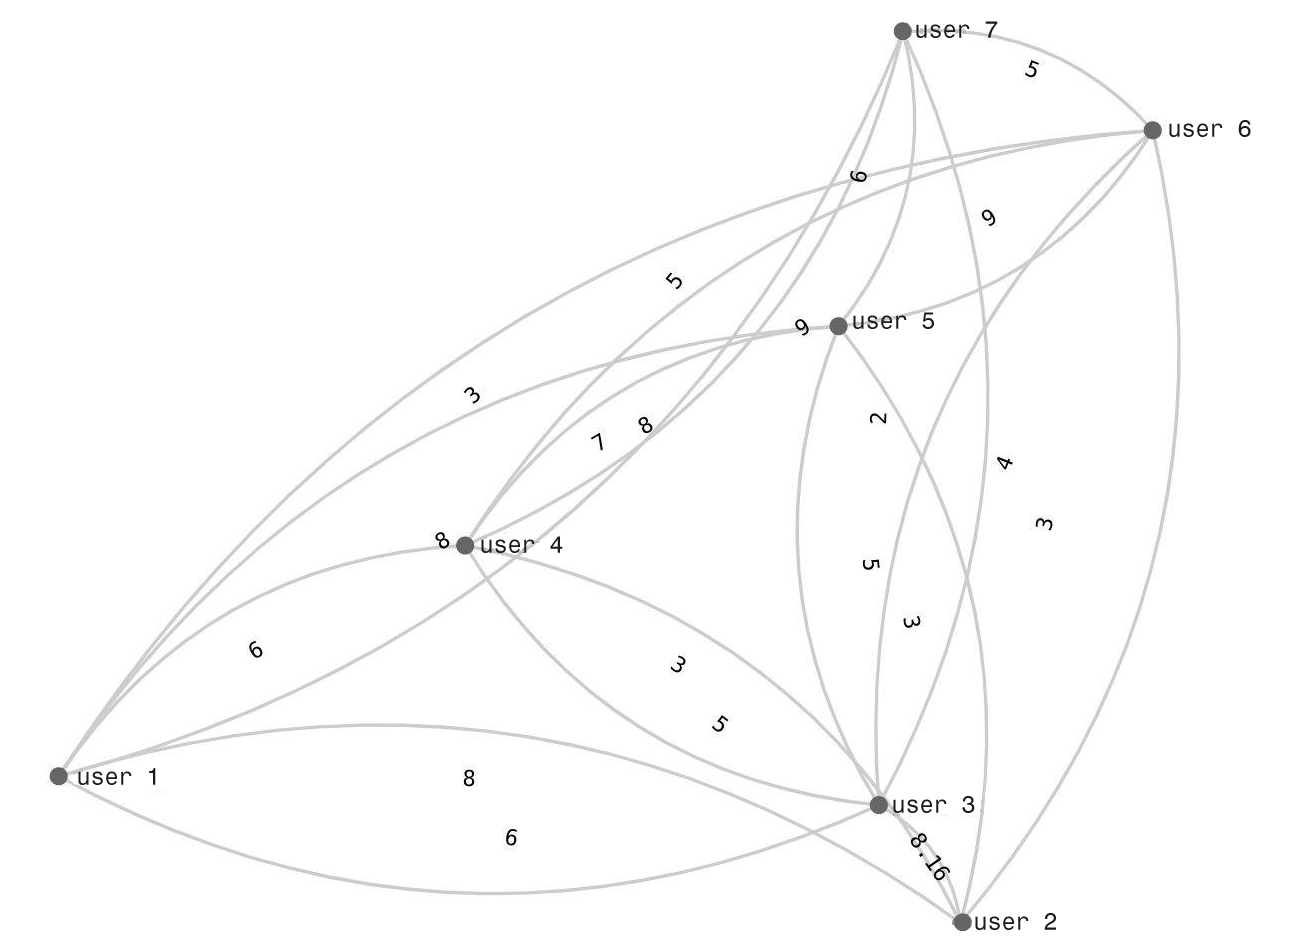
\includegraphics[width=12cm]{grafo.png}
\caption{Um grafo com 5 nós e 6 arestas.}
\label{fig:grafo}
\end{figure}

Quando a relação entre dois nós é simétrica, ou seja, a relação entre o nó $A$ e o nó $B$ é idêntica, diz-se que o grafo é \emph{não orientado}. Quando a relação entre dois nós é assimétrica, portanto, $A$ tem uma relação com $B$, mas essa relação não equivale a $B$ para $A$, tem-se um \emph{dígrafo} ou um \emph{grafo orientado}.

Este trabalho utiliza o grafo não orientado pois este bem representa as relações de amizade recíprocas. Tal decisão é tomada pois, quando da sugestão de um novo contato, ambos vão ser apresentados reciprocamente, estabelecendo, portanto, uma relação mútua de interação.

Diversas áreas da ciência, desde a biologia à linguística, utilizam grafos para representar dados. A representação de objetos e suas relações é uma ferramenta frequente em várias pesquisas.

Na ciência da computação, o grafo é a uma estrutura de dados amplamente frequente e existem centenas de problemas computacionais definidos com o seu uso \cite{Cormen2009}. Um caso tradicional com solução utilizando grafos é a do caixeiro viajante. Neste problema, os nós do grafo são as localidades e as arestas têm o peso equivalente à distância entre as cidades. \citep{Dijkstra1959}, propôs o primeiro algoritmo para encontrar o caminho mais curto entre dois nós de um grafo. O algoritmo encontra um caminho curto, mas não necessariamente o mais curto. Vários trabalhos são realizados ainda hoje na busca pelo caminho mais curto em um grafo. Muitos desses trabalhos são baseados no algoritmo de Dijkstra.

Como estrutura de dados computacionais, existem várias modelagens conhecidas para representação de um grafo. \citep{Cormen2009}, cita duas formas fundamentais:

\begin{itemize}
\item A lista de adjacência
\item A matriz de adjacência
\end{itemize}

\begin{figure}[!htb]
\centering
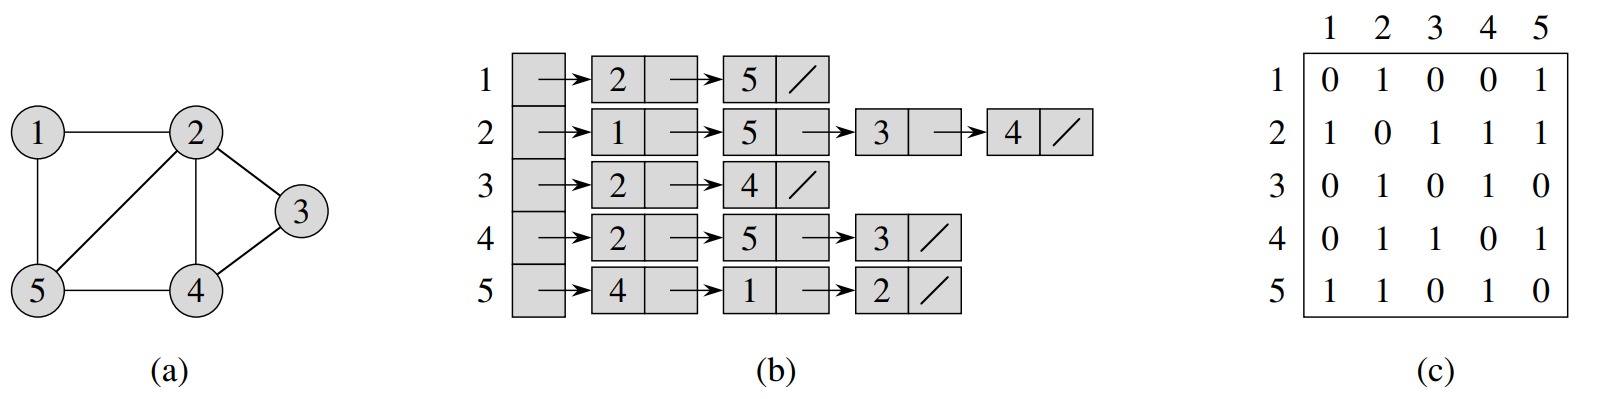
\includegraphics[width=16cm]{represent_grafo.png}
\caption{Duas representações de um grafo não direcionado. (\textbf{a}) Um grafo G com cinco nós e sete arestas. (\textbf{b}) A representação de uma lista de adjacência de G. (\textbf{c}) A representação de uma matriz de adjacência. Fonte: \cite{Cormen2009}, tradução dos autores.}
\label{fig:represent_grafo}
\end{figure}


\begin{figure}[!htb]
\centering
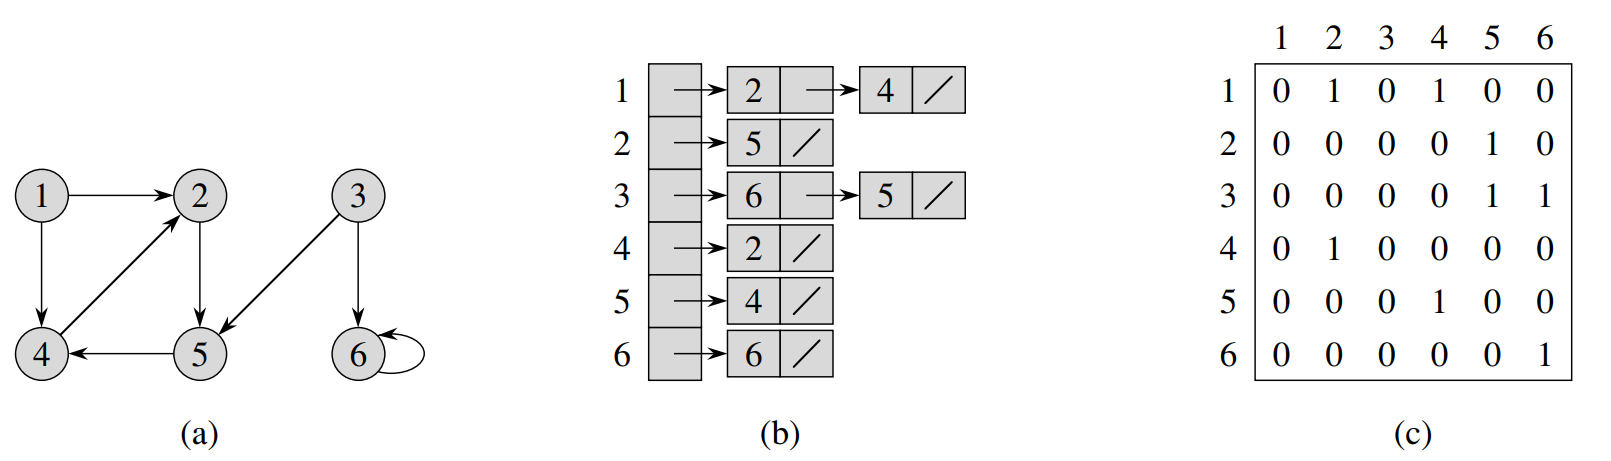
\includegraphics[width=16cm]{represent_grafo_ND.png}
\caption{Duas representações de um grafo direcionado. (\textbf{a}) Um grafo G com seis nós e oito arestas. (\textbf{b}) A representação de uma lista de adjacência de G. (\textbf{c}) A representação de uma matriz de adjacência. Fonte: \cite{Cormen2009}, tradução dos autores.}
\label{fig:represent_grafo_ND}
\end{figure}

\FloatBarrier

A Figura \ref{fig:represent_grafo}, ilustra um grafo $G$ como um diagrama, como uma lista de adjacência e como uma matriz de adjacência. A implementação computacional de um grafo pode ser a partir de uma lista de adjacência. Desse modo Um grafo $G = (N, E)$ consiste de uma lista de listas de nós, uma lista para cada nó em N. Para cada nó em G, tem-se uma lista dos nós vizinhos. Essa lista também pode conter somente um ponteiro para os nós vizinhos. Normalmente é suficiente armazenar os nós vizinhos em ordem arbitrária pois será o peso da aresta que determinará uma hierarquia entre os nós vizinhos, não a ordem pela qual eles foram adicionados nem qualquer outro atributo.
			% introdução
\chapter{Fundamentação Teórica}
\label{cap:fund}

% figuras estão no subdiretório "figuras/" dentro deste capítulo
\graphicspath{\currfiledir/figuras/}

Nesta parte, há a exposição das definições e histórico de redes sociais, algoritmos de recomendação e as definições matemáticas e computacionais de grafo. Esses três itens relacionam-se intrinsicamente com este trabalho, por isso, buscamos esclarecê-los o suficiente neste capítulo de maneira que as relações destes tópicos com o objetivo geral estejam fundamentadas.


\section{Redes Sociais}

% \begin{itemize}
% \item Histórico de redes sociais
% \item Tipos de redes sociais
% \item Redes parecidas com nosso trabalho
% \item Análises de tempo despendido em redes sociais.
% \end{itemize}

Desde a invenção da internet em 1991, mais e mais aplicações vem sendo criadas para facilitar e estimular os relacionamentos virtuais. As redes sociais virtuais tiveram início em 1997 com o site \emph{Six Degrees}, \citep{terrel17}. \emph{Six Degrees} é nomeado em referência ao estudo de \cite{milgram67}, que teorizava que são necessários seis laços de amizade para que quaisquer pessoas estejam conectadas. \emph{Six Degrees} teve seu fim em 2001, mas iniciou o processo de popularização das redes sociais e é considerado a primeira rede social pois permitia que as pessoas criassem seus perfis individuais e adicionar outros contatos à sua rede. Teve 3,5 milhões de usuários no seu auge.

Entre as precursoras está também a rede especializada em relacionamentos profissionais, \emph{LinkedIn}. Foi criada no final de 2002 e tem, desde então, seu objetivo principal em criar conexões entre profissionais, estudantes e corporações. O \emph{LinkedIn} é, ainda hoje, a rede mais popular neste nicho com mais de 500 milhões de usuários.

A rede mais popular atualmente, segundo \cite{lua19}, é o Facebook com 2,23 milhões de usuários ativos mensalmente. O Facebook foi criado em 2004 como uma rede específica para estudantes da Universidade de Harvard. Em 2006 foi aberta ao público e em 2008 já era a rede social mais visitada do mundo.

Há também redes especializadas em outros tipos de conexão ou outras maneiras de publicar conteúdo. O YouTube é uma rede social especializada na divulgação de vídeos criados pelos usuários. O Twitter, distingue-se das outras redes por iniciar suas atividades permitindo apenas a publicação de textos com, no máximo, 140 caracteres. Este limite foi dobrado posteriormente, mas o foco ainda mantém-se em pequenas postagens.

Por fim, há as redes especializadas em relacionamentos românticos. O Tinder, o Happn e o OKCupid são exemplos de redes sociais direcionadas à criação de relacionamentos íntimos entre os usuários. O sistema desenvolvido neste trabalho enquadra-se nesta categoria pois tem o objetivo de colocar usuários em contato com pessoas desconhecidas que têm potencial para formarem amizades ou até mesmo casais.

No Brasil, 66\% da população tem acesso à internet segundo \cite{wearesocial18}. Dentre os usuários da internet 93\% são ativos em alguma rede social.
Segundo \cite{wearesocial18}, o brasileiro despende, em média, 3h39min por dia em alguma rede social. Este tempo é passado em contato com informações e pessoas de várias culturas diferentes. Muitas vezes as interações despertam sentimentos indesejados e a informação divulgada não é completamente conexa à realidade.

Por essa razão, mais e mais redes sociais oferecem a oportunidade, muitas vezes compulsoriamente, do usuário ser exposto somente à pessoas e conteúdos que tenham afinidade com seu perfil. Na busca por uma experiência agradável, as sugestões de conteúdo e contatos vão ao encontro da necessidade do ser humano de se socializar. E participar de uma rede social, seja ela física ou virtual, faz parte das necessidades básicas apontadas por \cite{Maslow1943}, ao definir uma hierarquia para as necessidades básicas do ser humano.

De uma maneira ou de outra, todas as redes sociais tem seu foco no conteúdo gerado pelos usuários. Porém, grande parte da monetização empregada refere-se à divulgação de peças publicitárias pagas por empresas particulares e públicas. Dentro deste escopo, são utilizados algoritmos que tomam em conta os interesses dos usuários para fazer sugestões de conteúdo publicitário. Há vários métodos para relacionar os dados produzidos pelos usuários para gerar sugestões, sejam elas de conteúdo, publicidade ou novos contatos.

%=====================================================

\section{Algoritmos de Recomendação}

% \begin{itemize}
% \item Como sugerir novos contatos.
% \item Como as outras redes fazem isso.
% 
% \end{itemize}


Quando um usuário acessa um sistema qualquer que lhe oferece itens, por exemplo, livros, um sistema de recomendação pode lhe proporcionar a conveniência de sugerir-lhe um livro mais adequado para o seu gosto quando a quantidade de opções disponíveis é opressivamente vasta, diz \cite{Ricci2010}.

Esses itens, são quaisquer coisas que podem ser sugeridas ao usuário, sejam produtos, serviços, notícias, publicidade, ou, no caso deste trabalho, outros usuários com potencial para tornarem-se amizades.

Para \cite{Ricci2010}, a forma mais simples de um sistema de recomendação é uma lista com itens ordenados pela similaridade com o usuário que receberá a recomendação. Os sistemas de sugestão analisam vários tipos de dados por diversos métodos diferentes para encontrar os itens mais adequados para cada usuário. De acordo com \cite{Ricci2010}, os primeiros algoritmos de recomendação utilizavam dados gerados por recomendações feitas pela comunidade de usuários. Esse método comparava gostos similares entre os usuários e recomendava itens ainda não consumidos por alguns usuários. A este método dá-se o nome de Filtragem Colaborativa \citep{goldberg92}.

Desde os anos 1990, a perseguição por sistemas de recomendações cada vez mais eficientes impulsionou o surgimento do Prêmio Netflix em 2006, \citep{netflix}. Neste concurso, a empresa Netflix propôs pagar um prêmio de US\$1.000.000 para quem elaborasse um sistema que pudesse melhorar em, pelo menos, 10\% a acurácia do sistema que estava em uso à época. O time \emph{BellKor's Pragmatic Chaos}, venceu a disputa empregando diversos algoritmos e métodos de classificação mesclados em um mesmo sistema, \citep{Bell}. 

Entre as possibilidades de métodos e algoritmos que podem ser empregados em um sistema de recomendação, podemos ressaltar, baseados no texto de \cite{Recommendation}, as seguintes:

\begin{itemize}
\item Filtragem colaborativa
\item Filtragem baseada em conteúdo
\item Recomendação baseada em conhecimento
\end{itemize}

A filtragem colaborativa, como já mencionado, leva em conta as preferências já informadas pelos usuários para compará-las e sugerir novas possibilidades de itens. Tem a tendência de sugerir itens que já são apreciados por usuários que, de alguma maneira, já se relacionam, seja por interesses definidos, grupos específicos ou até mesmo por parentesco.

A filtragem baseada em conteúdo toma por verdadeira a afirmação de que os usuários que já demonstraram interesse por um tópico somente serão agradados por tópicos semelhantes e não podem ser instigados por assuntos fora do escopo do que já foi definido como interesse inicialmente. Dessa maneira, o sistema considera de que um usuário que declarou interesse por filmes deve receber sugestões de itens relacionados a este tema. É claro que este método tem a fraqueza de não sugerir novos assuntos que, potencialmente, despertariam o interesse do usuário.

Finalmente, a recomendação baseada em conhecimento,  que toma em conta regras de restrições de interesse definidas no sistema e os aplica à lista de itens disponíveis. Desse modo, os itens são sugeridos a partir do resultado da filtragem realizada a partir das regras definidas. A definição de tais regras passa por análises semânticas do conteúdo disponível no sistema que diga respeito ao usuário. O sistema desenvolvido neste trabalho assemelha-se a uma recomendação baseada em conhecimento no sentido de que a regra definida para relacionar os itens será uma equação determinística que calcula um valor de proximidade entre dois itens.

Os vários métodos de recomendação tem sua acurácia diretamente influenciada pela quantidade de informação disponível sobre os usuários ou gerada pelos usuários. Quanto maior a quantidade de informação disponível, maior a acurácia e, em linhas gerais, menor a performance do sistema, uma vez que o tempo de processamento da informação é incrementado. Por essa razão, boas soluções são baseadas em aprendizado de máquina e inteligência artificial. O emprego dessas tecnologias tem o objetivo de melhorar a performance e a acurácia das sugestões.

%=====================================================

\section{Grafo}
% \begin{itemize}
% \item O que é grafo - \emph{Fonte básica de definição de grafo LIVRO??}
% \item Quantos tipos de grafo existem.
% \item Aplicações comuns de grafo
% \item Algoritmos que usam grafos
% \end{itemize}

O conceito matemático de grafo parte de abstrações de situações da vida real onde objetos ou pessoas representadas por pontos e suas conexões e interações são representadas por linhas \cite{Bondy08}. Numa rede social, as pessoas são esses pontos, que convencionalmente são chamados de nós, e suas relações com outras pessoas são representadas por linhas, chamadas de arestas. Um grafo é uma tripla ordenada $G=(N(G), A(G), \psi _{G})$, que consiste de um conjunto não vazio $N(G)$ de nós, um conjunto $A(G)$, diferente de $N(G)$, de arestas, e uma \emph{função de incidência} $\psi_{G}$ que associa a cada nó de $G$ um par não ordenado de nós de $G$. Se $e$ é uma aresta de $G$ e $u$ e $v$ são arestas de tal modo que $\psi_{G}(e) = un$, então $e$ é dito que \emph{une} $u$ e $n$ \cite{Bondy08}.

\emph{Exemplo}

\begin{equation}
G=(N(G), A(G), \psi _{G})
\label{eq:grafo}
\end{equation}

\emph{onde}

\begin{equation}
N(G)={n_{1}, n_{2}, n_{3}, n_{4}, n_{5}}
\label{eq:grafo2}
\end{equation}

\emph{e $\psi_{G}$ é definido por}

\begin{equation}
\begin{split}
\psi_{G}(a_{1}) = n_{1}n_{2}, \psi_{G}(a_{2} = n_{2}n_{3}, \psi_{G}(a_{3}) = n_{3}n_{3}, \psi_{G}(a_{4}) = n_{2}n_{4} \\
\psi_{G}(a_{5}) = n_{2}n_{4}, \psi_{G}(a_{6} = n_{4}n_{5}, \psi_{G}(n_{8}) = n_{2}n_{5}, \psi_{G}(a_{4}) = n_{2}n_{4}
\label{eq:grafo3}
\end{split}
\end{equation}

Grafos têm este nome pois podem ser representadas graficamente, segundo \cite{Bondy08}. A Figura \ref{fig:grafo}, é um diagrama que representa um grafo com 5 nós e 6 arestas. Nesta Figura, os nós têm identificação - letras - e as arestas tem um \emph{peso}. O peso das arestas pode ser usado para representar a força da ligação entre os nós ou até mesmo a distância entre os nós. A convenção tomada neste caso depende do contexto e da aplicação do grafo.

\begin{figure}[!htb]
\centering
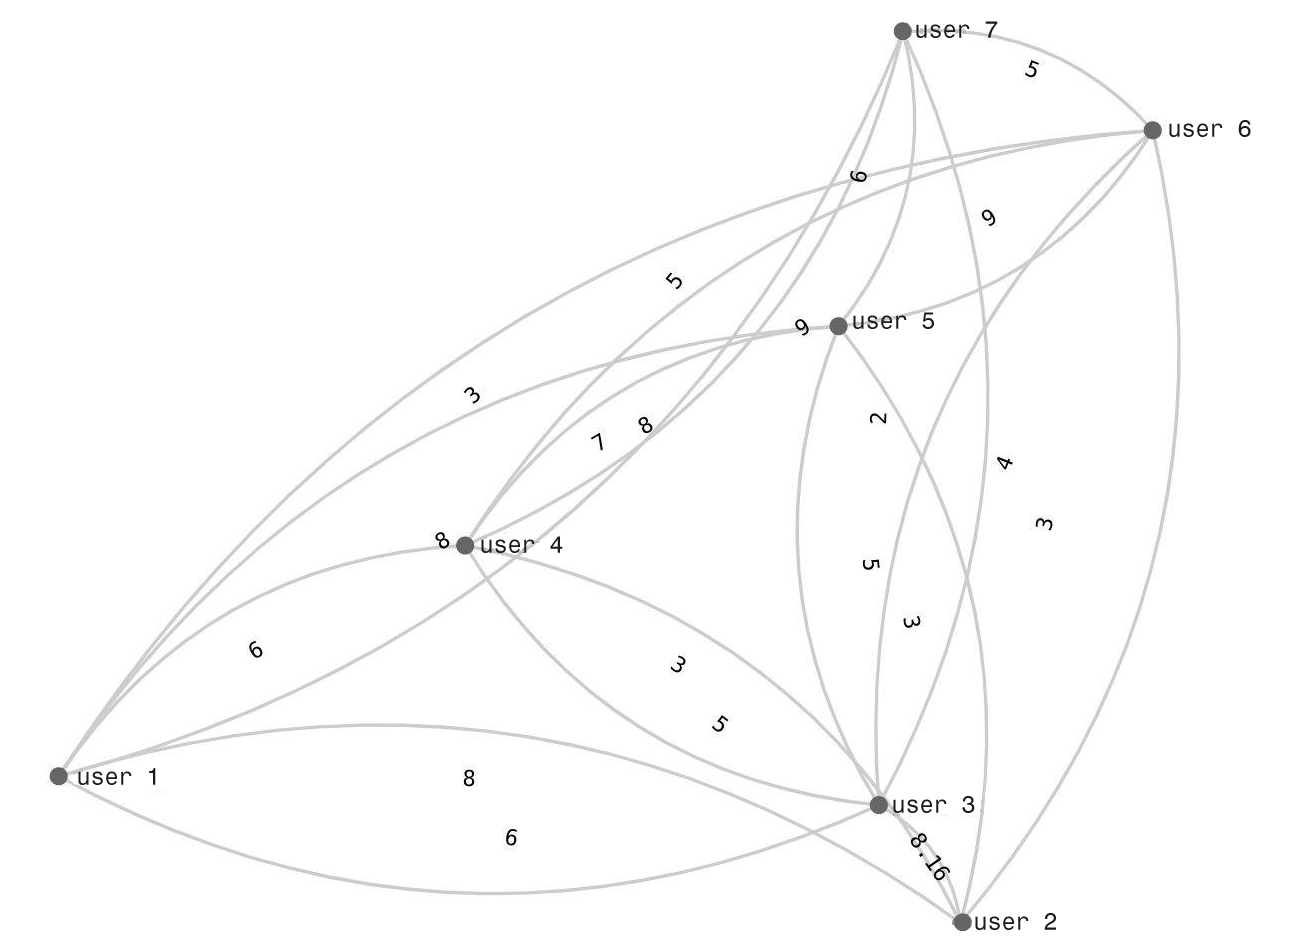
\includegraphics[width=12cm]{grafo.png}
\caption{Um grafo com 5 nós e 6 arestas.}
\label{fig:grafo}
\end{figure}

Quando a relação entre dois nós é simétrica, ou seja, a relação entre o nó $A$ e o nó $B$ é idêntica, diz-se que o grafo é \emph{não orientado}. Quando a relação entre dois nós é assimétrica, portanto, $A$ tem uma relação com $B$, mas essa relação não equivale a $B$ para $A$, tem-se um \emph{dígrafo} ou um \emph{grafo orientado}.

Este trabalho utiliza o grafo não orientado pois este bem representa as relações de amizade recíprocas. Tal decisão é tomada pois, quando da sugestão de um novo contato, ambos vão ser apresentados reciprocamente, estabelecendo, portanto, uma relação mútua de interação.

Diversas áreas da ciência, desde a biologia à linguística, utilizam grafos para representar dados. A representação de objetos e suas relações é uma ferramenta frequente em várias pesquisas.

Na ciência da computação, o grafo é a uma estrutura de dados amplamente frequente e existem centenas de problemas computacionais definidos com o seu uso \cite{Cormen2009}. Um caso tradicional com solução utilizando grafos é a do caixeiro viajante. Neste problema, os nós do grafo são as localidades e as arestas têm o peso equivalente à distância entre as cidades. \citep{Dijkstra1959}, propôs o primeiro algoritmo para encontrar o caminho mais curto entre dois nós de um grafo. O algoritmo encontra um caminho curto, mas não necessariamente o mais curto. Vários trabalhos são realizados ainda hoje na busca pelo caminho mais curto em um grafo. Muitos desses trabalhos são baseados no algoritmo de Dijkstra.

Como estrutura de dados computacionais, existem várias modelagens conhecidas para representação de um grafo. \citep{Cormen2009}, cita duas formas fundamentais:

\begin{itemize}
\item A lista de adjacência
\item A matriz de adjacência
\end{itemize}

\begin{figure}[!htb]
\centering
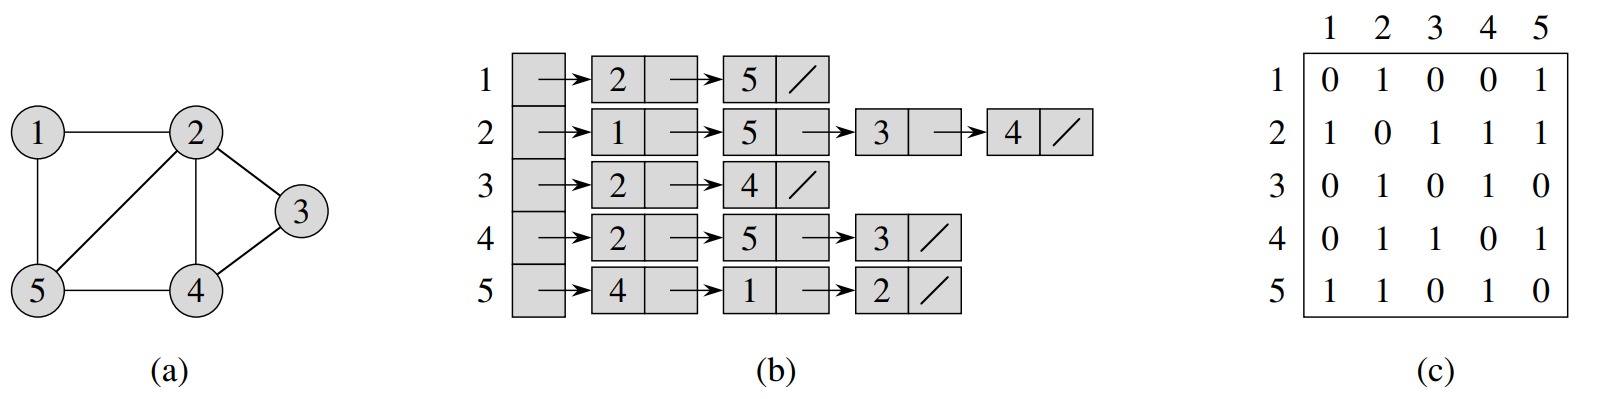
\includegraphics[width=16cm]{represent_grafo.png}
\caption{Duas representações de um grafo não direcionado. (\textbf{a}) Um grafo G com cinco nós e sete arestas. (\textbf{b}) A representação de uma lista de adjacência de G. (\textbf{c}) A representação de uma matriz de adjacência. Fonte: \cite{Cormen2009}, tradução dos autores.}
\label{fig:represent_grafo}
\end{figure}


\begin{figure}[!htb]
\centering
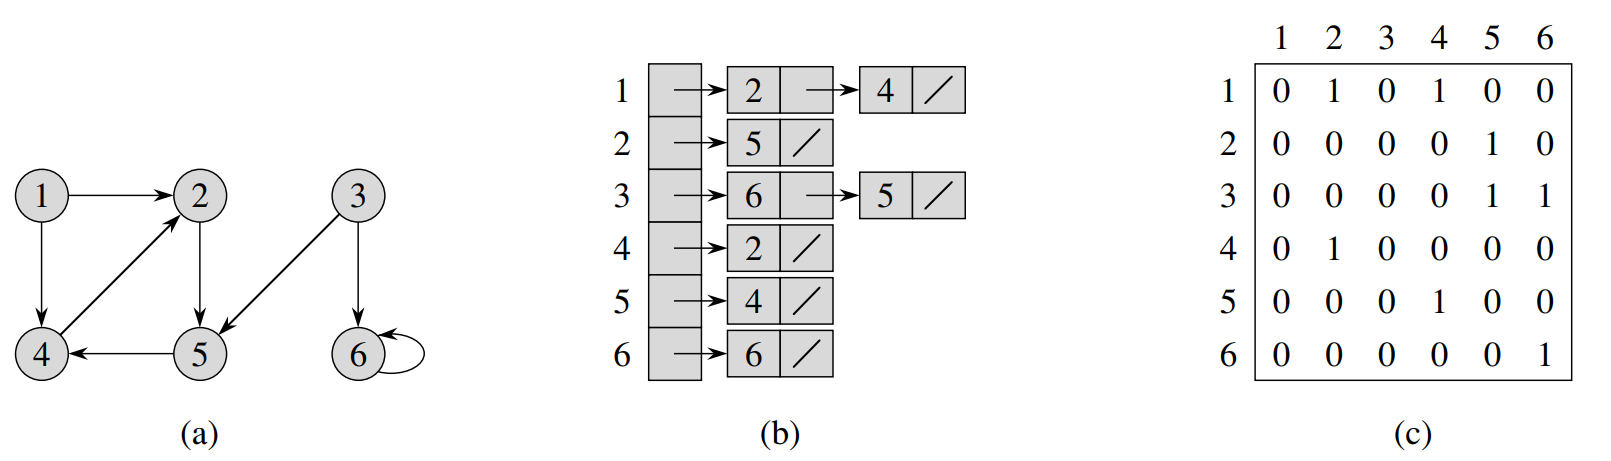
\includegraphics[width=16cm]{represent_grafo_ND.png}
\caption{Duas representações de um grafo direcionado. (\textbf{a}) Um grafo G com seis nós e oito arestas. (\textbf{b}) A representação de uma lista de adjacência de G. (\textbf{c}) A representação de uma matriz de adjacência. Fonte: \cite{Cormen2009}, tradução dos autores.}
\label{fig:represent_grafo_ND}
\end{figure}

\FloatBarrier

A Figura \ref{fig:represent_grafo}, ilustra um grafo $G$ como um diagrama, como uma lista de adjacência e como uma matriz de adjacência. A implementação computacional de um grafo pode ser a partir de uma lista de adjacência. Desse modo Um grafo $G = (N, E)$ consiste de uma lista de listas de nós, uma lista para cada nó em N. Para cada nó em G, tem-se uma lista dos nós vizinhos. Essa lista também pode conter somente um ponteiro para os nós vizinhos. Normalmente é suficiente armazenar os nós vizinhos em ordem arbitrária pois será o peso da aresta que determinará uma hierarquia entre os nós vizinhos, não a ordem pela qual eles foram adicionados nem qualquer outro atributo.
		% fundamentação teórica
%\chapter{Fundamentação Teórica}
\label{cap:fund}

% figuras estão no subdiretório "figuras/" dentro deste capítulo
\graphicspath{\currfiledir/figuras/}

Nesta parte, há a exposição das definições e histórico de redes sociais, algoritmos de recomendação e as definições matemáticas e computacionais de grafo. Esses três itens relacionam-se intrinsicamente com este trabalho, por isso, buscamos esclarecê-los o suficiente neste capítulo de maneira que as relações destes tópicos com o objetivo geral estejam fundamentadas.


\section{Redes Sociais}

% \begin{itemize}
% \item Histórico de redes sociais
% \item Tipos de redes sociais
% \item Redes parecidas com nosso trabalho
% \item Análises de tempo despendido em redes sociais.
% \end{itemize}

Desde a invenção da internet em 1991, mais e mais aplicações vem sendo criadas para facilitar e estimular os relacionamentos virtuais. As redes sociais virtuais tiveram início em 1997 com o site \emph{Six Degrees}, \citep{terrel17}. \emph{Six Degrees} é nomeado em referência ao estudo de \cite{milgram67}, que teorizava que são necessários seis laços de amizade para que quaisquer pessoas estejam conectadas. \emph{Six Degrees} teve seu fim em 2001, mas iniciou o processo de popularização das redes sociais e é considerado a primeira rede social pois permitia que as pessoas criassem seus perfis individuais e adicionar outros contatos à sua rede. Teve 3,5 milhões de usuários no seu auge.

Entre as precursoras está também a rede especializada em relacionamentos profissionais, \emph{LinkedIn}. Foi criada no final de 2002 e tem, desde então, seu objetivo principal em criar conexões entre profissionais, estudantes e corporações. O \emph{LinkedIn} é, ainda hoje, a rede mais popular neste nicho com mais de 500 milhões de usuários.

A rede mais popular atualmente, segundo \cite{lua19}, é o Facebook com 2,23 milhões de usuários ativos mensalmente. O Facebook foi criado em 2004 como uma rede específica para estudantes da Universidade de Harvard. Em 2006 foi aberta ao público e em 2008 já era a rede social mais visitada do mundo.

Há também redes especializadas em outros tipos de conexão ou outras maneiras de publicar conteúdo. O YouTube é uma rede social especializada na divulgação de vídeos criados pelos usuários. O Twitter, distingue-se das outras redes por iniciar suas atividades permitindo apenas a publicação de textos com, no máximo, 140 caracteres. Este limite foi dobrado posteriormente, mas o foco ainda mantém-se em pequenas postagens.

Por fim, há as redes especializadas em relacionamentos românticos. O Tinder, o Happn e o OKCupid são exemplos de redes sociais direcionadas à criação de relacionamentos íntimos entre os usuários. O sistema desenvolvido neste trabalho enquadra-se nesta categoria pois tem o objetivo de colocar usuários em contato com pessoas desconhecidas que têm potencial para formarem amizades ou até mesmo casais.

No Brasil, 66\% da população tem acesso à internet segundo \cite{wearesocial18}. Dentre os usuários da internet 93\% são ativos em alguma rede social.
Segundo \cite{wearesocial18}, o brasileiro despende, em média, 3h39min por dia em alguma rede social. Este tempo é passado em contato com informações e pessoas de várias culturas diferentes. Muitas vezes as interações despertam sentimentos indesejados e a informação divulgada não é completamente conexa à realidade.

Por essa razão, mais e mais redes sociais oferecem a oportunidade, muitas vezes compulsoriamente, do usuário ser exposto somente à pessoas e conteúdos que tenham afinidade com seu perfil. Na busca por uma experiência agradável, as sugestões de conteúdo e contatos vão ao encontro da necessidade do ser humano de se socializar. E participar de uma rede social, seja ela física ou virtual, faz parte das necessidades básicas apontadas por \cite{Maslow1943}, ao definir uma hierarquia para as necessidades básicas do ser humano.

De uma maneira ou de outra, todas as redes sociais tem seu foco no conteúdo gerado pelos usuários. Porém, grande parte da monetização empregada refere-se à divulgação de peças publicitárias pagas por empresas particulares e públicas. Dentro deste escopo, são utilizados algoritmos que tomam em conta os interesses dos usuários para fazer sugestões de conteúdo publicitário. Há vários métodos para relacionar os dados produzidos pelos usuários para gerar sugestões, sejam elas de conteúdo, publicidade ou novos contatos.

%=====================================================

\section{Algoritmos de Recomendação}

% \begin{itemize}
% \item Como sugerir novos contatos.
% \item Como as outras redes fazem isso.
% 
% \end{itemize}


Quando um usuário acessa um sistema qualquer que lhe oferece itens, por exemplo, livros, um sistema de recomendação pode lhe proporcionar a conveniência de sugerir-lhe um livro mais adequado para o seu gosto quando a quantidade de opções disponíveis é opressivamente vasta, diz \cite{Ricci2010}.

Esses itens, são quaisquer coisas que podem ser sugeridas ao usuário, sejam produtos, serviços, notícias, publicidade, ou, no caso deste trabalho, outros usuários com potencial para tornarem-se amizades.

Para \cite{Ricci2010}, a forma mais simples de um sistema de recomendação é uma lista com itens ordenados pela similaridade com o usuário que receberá a recomendação. Os sistemas de sugestão analisam vários tipos de dados por diversos métodos diferentes para encontrar os itens mais adequados para cada usuário. De acordo com \cite{Ricci2010}, os primeiros algoritmos de recomendação utilizavam dados gerados por recomendações feitas pela comunidade de usuários. Esse método comparava gostos similares entre os usuários e recomendava itens ainda não consumidos por alguns usuários. A este método dá-se o nome de Filtragem Colaborativa \citep{goldberg92}.

Desde os anos 1990, a perseguição por sistemas de recomendações cada vez mais eficientes impulsionou o surgimento do Prêmio Netflix em 2006, \citep{netflix}. Neste concurso, a empresa Netflix propôs pagar um prêmio de US\$1.000.000 para quem elaborasse um sistema que pudesse melhorar em, pelo menos, 10\% a acurácia do sistema que estava em uso à época. O time \emph{BellKor's Pragmatic Chaos}, venceu a disputa empregando diversos algoritmos e métodos de classificação mesclados em um mesmo sistema, \citep{Bell}. 

Entre as possibilidades de métodos e algoritmos que podem ser empregados em um sistema de recomendação, podemos ressaltar, baseados no texto de \cite{Recommendation}, as seguintes:

\begin{itemize}
\item Filtragem colaborativa
\item Filtragem baseada em conteúdo
\item Recomendação baseada em conhecimento
\end{itemize}

A filtragem colaborativa, como já mencionado, leva em conta as preferências já informadas pelos usuários para compará-las e sugerir novas possibilidades de itens. Tem a tendência de sugerir itens que já são apreciados por usuários que, de alguma maneira, já se relacionam, seja por interesses definidos, grupos específicos ou até mesmo por parentesco.

A filtragem baseada em conteúdo toma por verdadeira a afirmação de que os usuários que já demonstraram interesse por um tópico somente serão agradados por tópicos semelhantes e não podem ser instigados por assuntos fora do escopo do que já foi definido como interesse inicialmente. Dessa maneira, o sistema considera de que um usuário que declarou interesse por filmes deve receber sugestões de itens relacionados a este tema. É claro que este método tem a fraqueza de não sugerir novos assuntos que, potencialmente, despertariam o interesse do usuário.

Finalmente, a recomendação baseada em conhecimento,  que toma em conta regras de restrições de interesse definidas no sistema e os aplica à lista de itens disponíveis. Desse modo, os itens são sugeridos a partir do resultado da filtragem realizada a partir das regras definidas. A definição de tais regras passa por análises semânticas do conteúdo disponível no sistema que diga respeito ao usuário. O sistema desenvolvido neste trabalho assemelha-se a uma recomendação baseada em conhecimento no sentido de que a regra definida para relacionar os itens será uma equação determinística que calcula um valor de proximidade entre dois itens.

Os vários métodos de recomendação tem sua acurácia diretamente influenciada pela quantidade de informação disponível sobre os usuários ou gerada pelos usuários. Quanto maior a quantidade de informação disponível, maior a acurácia e, em linhas gerais, menor a performance do sistema, uma vez que o tempo de processamento da informação é incrementado. Por essa razão, boas soluções são baseadas em aprendizado de máquina e inteligência artificial. O emprego dessas tecnologias tem o objetivo de melhorar a performance e a acurácia das sugestões.

%=====================================================

\section{Grafo}
% \begin{itemize}
% \item O que é grafo - \emph{Fonte básica de definição de grafo LIVRO??}
% \item Quantos tipos de grafo existem.
% \item Aplicações comuns de grafo
% \item Algoritmos que usam grafos
% \end{itemize}

O conceito matemático de grafo parte de abstrações de situações da vida real onde objetos ou pessoas representadas por pontos e suas conexões e interações são representadas por linhas \cite{Bondy08}. Numa rede social, as pessoas são esses pontos, que convencionalmente são chamados de nós, e suas relações com outras pessoas são representadas por linhas, chamadas de arestas. Um grafo é uma tripla ordenada $G=(N(G), A(G), \psi _{G})$, que consiste de um conjunto não vazio $N(G)$ de nós, um conjunto $A(G)$, diferente de $N(G)$, de arestas, e uma \emph{função de incidência} $\psi_{G}$ que associa a cada nó de $G$ um par não ordenado de nós de $G$. Se $e$ é uma aresta de $G$ e $u$ e $v$ são arestas de tal modo que $\psi_{G}(e) = un$, então $e$ é dito que \emph{une} $u$ e $n$ \cite{Bondy08}.

\emph{Exemplo}

\begin{equation}
G=(N(G), A(G), \psi _{G})
\label{eq:grafo}
\end{equation}

\emph{onde}

\begin{equation}
N(G)={n_{1}, n_{2}, n_{3}, n_{4}, n_{5}}
\label{eq:grafo2}
\end{equation}

\emph{e $\psi_{G}$ é definido por}

\begin{equation}
\begin{split}
\psi_{G}(a_{1}) = n_{1}n_{2}, \psi_{G}(a_{2} = n_{2}n_{3}, \psi_{G}(a_{3}) = n_{3}n_{3}, \psi_{G}(a_{4}) = n_{2}n_{4} \\
\psi_{G}(a_{5}) = n_{2}n_{4}, \psi_{G}(a_{6} = n_{4}n_{5}, \psi_{G}(n_{8}) = n_{2}n_{5}, \psi_{G}(a_{4}) = n_{2}n_{4}
\label{eq:grafo3}
\end{split}
\end{equation}

Grafos têm este nome pois podem ser representadas graficamente, segundo \cite{Bondy08}. A Figura \ref{fig:grafo}, é um diagrama que representa um grafo com 5 nós e 6 arestas. Nesta Figura, os nós têm identificação - letras - e as arestas tem um \emph{peso}. O peso das arestas pode ser usado para representar a força da ligação entre os nós ou até mesmo a distância entre os nós. A convenção tomada neste caso depende do contexto e da aplicação do grafo.

\begin{figure}[!htb]
\centering
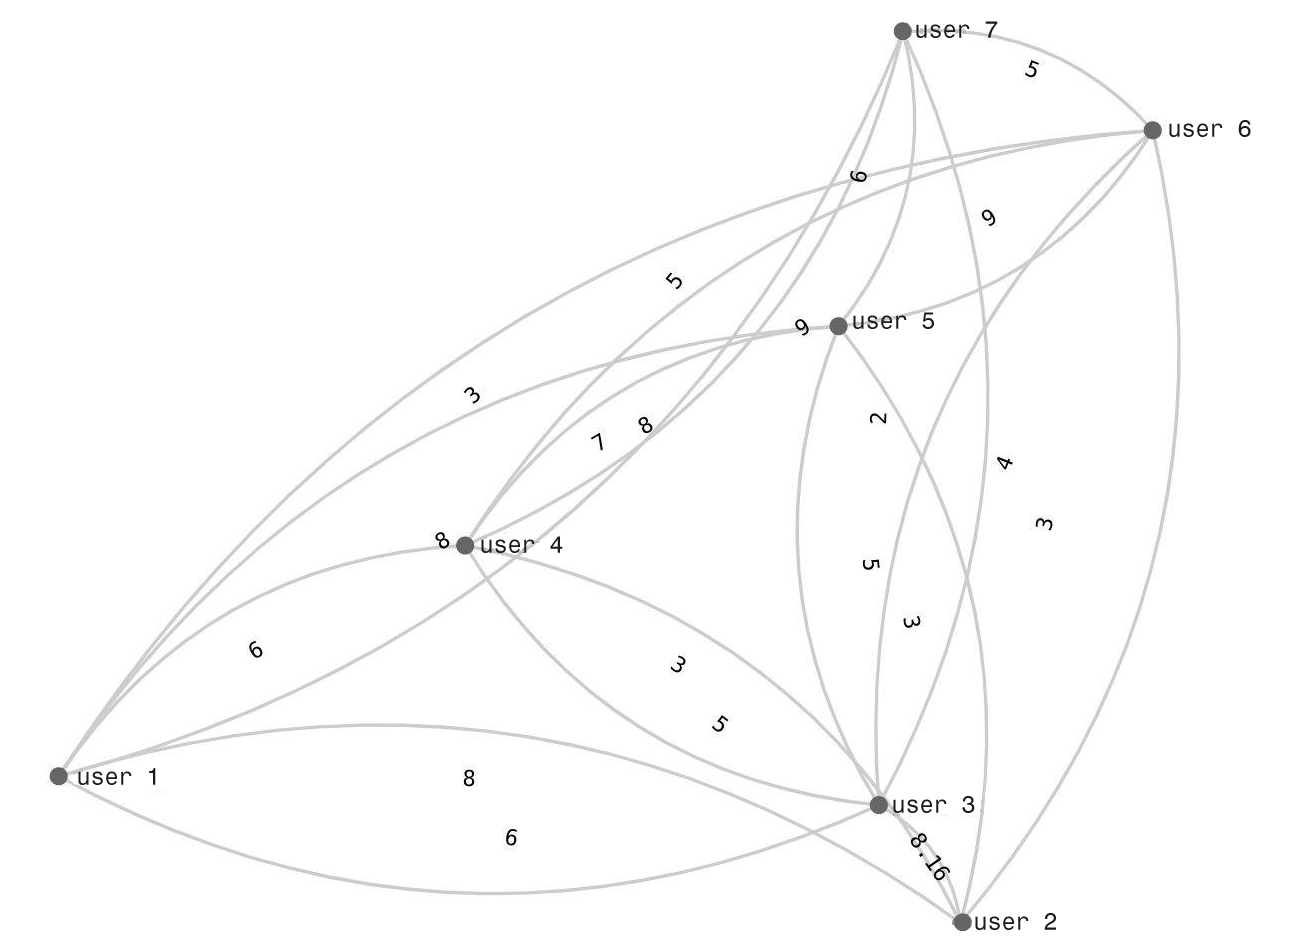
\includegraphics[width=12cm]{grafo.png}
\caption{Um grafo com 5 nós e 6 arestas.}
\label{fig:grafo}
\end{figure}

Quando a relação entre dois nós é simétrica, ou seja, a relação entre o nó $A$ e o nó $B$ é idêntica, diz-se que o grafo é \emph{não orientado}. Quando a relação entre dois nós é assimétrica, portanto, $A$ tem uma relação com $B$, mas essa relação não equivale a $B$ para $A$, tem-se um \emph{dígrafo} ou um \emph{grafo orientado}.

Este trabalho utiliza o grafo não orientado pois este bem representa as relações de amizade recíprocas. Tal decisão é tomada pois, quando da sugestão de um novo contato, ambos vão ser apresentados reciprocamente, estabelecendo, portanto, uma relação mútua de interação.

Diversas áreas da ciência, desde a biologia à linguística, utilizam grafos para representar dados. A representação de objetos e suas relações é uma ferramenta frequente em várias pesquisas.

Na ciência da computação, o grafo é a uma estrutura de dados amplamente frequente e existem centenas de problemas computacionais definidos com o seu uso \cite{Cormen2009}. Um caso tradicional com solução utilizando grafos é a do caixeiro viajante. Neste problema, os nós do grafo são as localidades e as arestas têm o peso equivalente à distância entre as cidades. \citep{Dijkstra1959}, propôs o primeiro algoritmo para encontrar o caminho mais curto entre dois nós de um grafo. O algoritmo encontra um caminho curto, mas não necessariamente o mais curto. Vários trabalhos são realizados ainda hoje na busca pelo caminho mais curto em um grafo. Muitos desses trabalhos são baseados no algoritmo de Dijkstra.

Como estrutura de dados computacionais, existem várias modelagens conhecidas para representação de um grafo. \citep{Cormen2009}, cita duas formas fundamentais:

\begin{itemize}
\item A lista de adjacência
\item A matriz de adjacência
\end{itemize}

\begin{figure}[!htb]
\centering
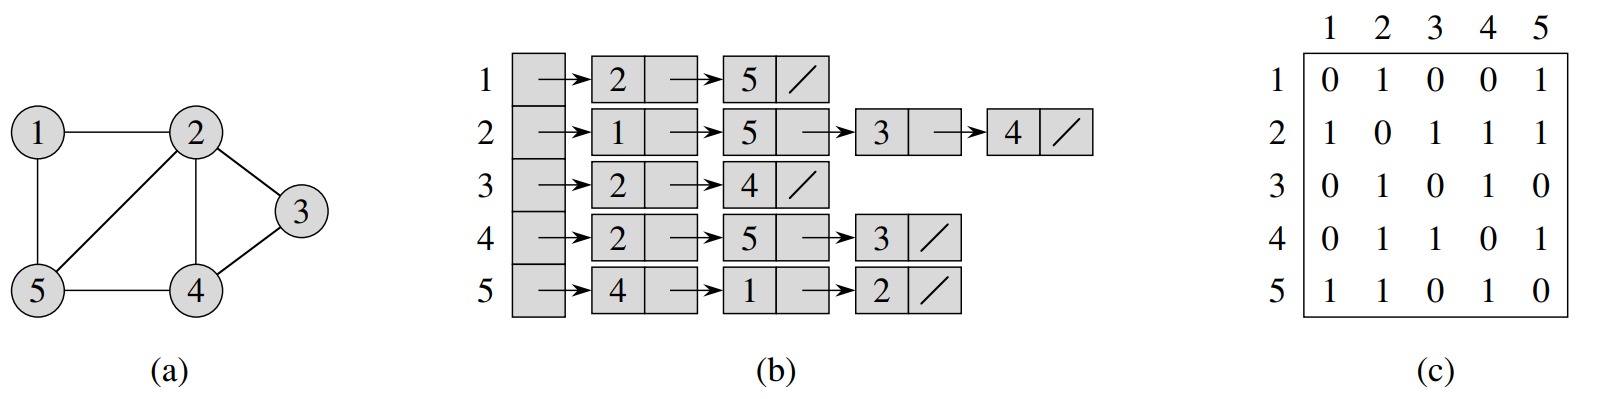
\includegraphics[width=16cm]{represent_grafo.png}
\caption{Duas representações de um grafo não direcionado. (\textbf{a}) Um grafo G com cinco nós e sete arestas. (\textbf{b}) A representação de uma lista de adjacência de G. (\textbf{c}) A representação de uma matriz de adjacência. Fonte: \cite{Cormen2009}, tradução dos autores.}
\label{fig:represent_grafo}
\end{figure}


\begin{figure}[!htb]
\centering
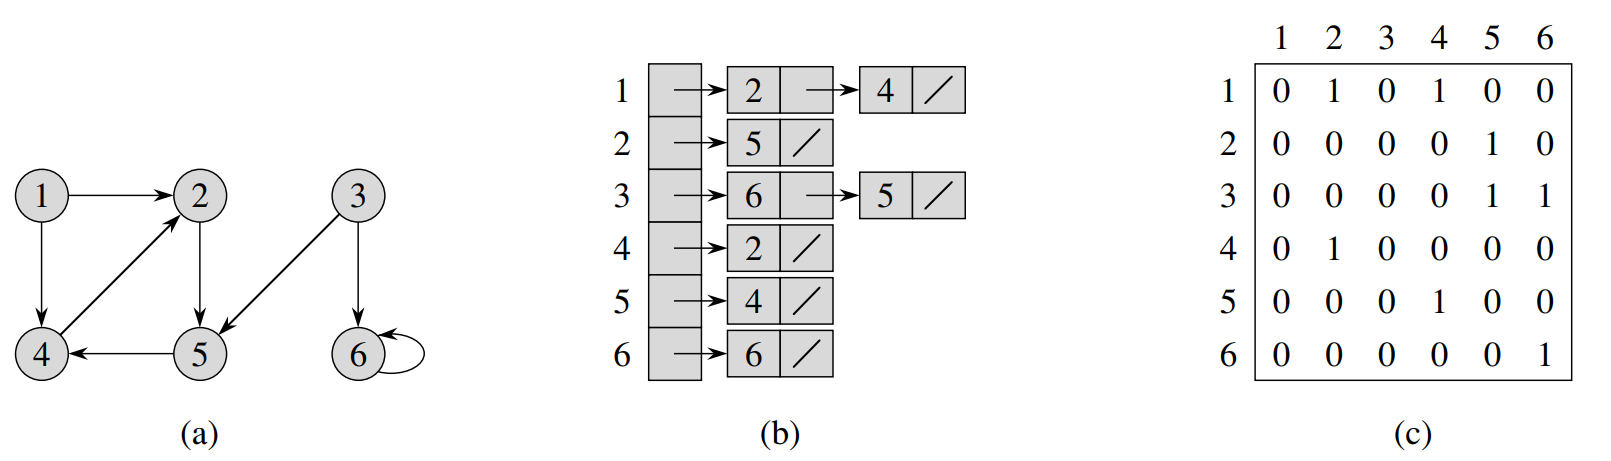
\includegraphics[width=16cm]{represent_grafo_ND.png}
\caption{Duas representações de um grafo direcionado. (\textbf{a}) Um grafo G com seis nós e oito arestas. (\textbf{b}) A representação de uma lista de adjacência de G. (\textbf{c}) A representação de uma matriz de adjacência. Fonte: \cite{Cormen2009}, tradução dos autores.}
\label{fig:represent_grafo_ND}
\end{figure}

\FloatBarrier

A Figura \ref{fig:represent_grafo}, ilustra um grafo $G$ como um diagrama, como uma lista de adjacência e como uma matriz de adjacência. A implementação computacional de um grafo pode ser a partir de uma lista de adjacência. Desse modo Um grafo $G = (N, E)$ consiste de uma lista de listas de nós, uma lista para cada nó em N. Para cada nó em G, tem-se uma lista dos nós vizinhos. Essa lista também pode conter somente um ponteiro para os nós vizinhos. Normalmente é suficiente armazenar os nós vizinhos em ordem arbitrária pois será o peso da aresta que determinará uma hierarquia entre os nós vizinhos, não a ordem pela qual eles foram adicionados nem qualquer outro atributo.
		% revisão bibliográfica (estado da arte)
%\chapter{Fundamentação Teórica}
\label{cap:fund}

% figuras estão no subdiretório "figuras/" dentro deste capítulo
\graphicspath{\currfiledir/figuras/}

Nesta parte, há a exposição das definições e histórico de redes sociais, algoritmos de recomendação e as definições matemáticas e computacionais de grafo. Esses três itens relacionam-se intrinsicamente com este trabalho, por isso, buscamos esclarecê-los o suficiente neste capítulo de maneira que as relações destes tópicos com o objetivo geral estejam fundamentadas.


\section{Redes Sociais}

% \begin{itemize}
% \item Histórico de redes sociais
% \item Tipos de redes sociais
% \item Redes parecidas com nosso trabalho
% \item Análises de tempo despendido em redes sociais.
% \end{itemize}

Desde a invenção da internet em 1991, mais e mais aplicações vem sendo criadas para facilitar e estimular os relacionamentos virtuais. As redes sociais virtuais tiveram início em 1997 com o site \emph{Six Degrees}, \citep{terrel17}. \emph{Six Degrees} é nomeado em referência ao estudo de \cite{milgram67}, que teorizava que são necessários seis laços de amizade para que quaisquer pessoas estejam conectadas. \emph{Six Degrees} teve seu fim em 2001, mas iniciou o processo de popularização das redes sociais e é considerado a primeira rede social pois permitia que as pessoas criassem seus perfis individuais e adicionar outros contatos à sua rede. Teve 3,5 milhões de usuários no seu auge.

Entre as precursoras está também a rede especializada em relacionamentos profissionais, \emph{LinkedIn}. Foi criada no final de 2002 e tem, desde então, seu objetivo principal em criar conexões entre profissionais, estudantes e corporações. O \emph{LinkedIn} é, ainda hoje, a rede mais popular neste nicho com mais de 500 milhões de usuários.

A rede mais popular atualmente, segundo \cite{lua19}, é o Facebook com 2,23 milhões de usuários ativos mensalmente. O Facebook foi criado em 2004 como uma rede específica para estudantes da Universidade de Harvard. Em 2006 foi aberta ao público e em 2008 já era a rede social mais visitada do mundo.

Há também redes especializadas em outros tipos de conexão ou outras maneiras de publicar conteúdo. O YouTube é uma rede social especializada na divulgação de vídeos criados pelos usuários. O Twitter, distingue-se das outras redes por iniciar suas atividades permitindo apenas a publicação de textos com, no máximo, 140 caracteres. Este limite foi dobrado posteriormente, mas o foco ainda mantém-se em pequenas postagens.

Por fim, há as redes especializadas em relacionamentos românticos. O Tinder, o Happn e o OKCupid são exemplos de redes sociais direcionadas à criação de relacionamentos íntimos entre os usuários. O sistema desenvolvido neste trabalho enquadra-se nesta categoria pois tem o objetivo de colocar usuários em contato com pessoas desconhecidas que têm potencial para formarem amizades ou até mesmo casais.

No Brasil, 66\% da população tem acesso à internet segundo \cite{wearesocial18}. Dentre os usuários da internet 93\% são ativos em alguma rede social.
Segundo \cite{wearesocial18}, o brasileiro despende, em média, 3h39min por dia em alguma rede social. Este tempo é passado em contato com informações e pessoas de várias culturas diferentes. Muitas vezes as interações despertam sentimentos indesejados e a informação divulgada não é completamente conexa à realidade.

Por essa razão, mais e mais redes sociais oferecem a oportunidade, muitas vezes compulsoriamente, do usuário ser exposto somente à pessoas e conteúdos que tenham afinidade com seu perfil. Na busca por uma experiência agradável, as sugestões de conteúdo e contatos vão ao encontro da necessidade do ser humano de se socializar. E participar de uma rede social, seja ela física ou virtual, faz parte das necessidades básicas apontadas por \cite{Maslow1943}, ao definir uma hierarquia para as necessidades básicas do ser humano.

De uma maneira ou de outra, todas as redes sociais tem seu foco no conteúdo gerado pelos usuários. Porém, grande parte da monetização empregada refere-se à divulgação de peças publicitárias pagas por empresas particulares e públicas. Dentro deste escopo, são utilizados algoritmos que tomam em conta os interesses dos usuários para fazer sugestões de conteúdo publicitário. Há vários métodos para relacionar os dados produzidos pelos usuários para gerar sugestões, sejam elas de conteúdo, publicidade ou novos contatos.

%=====================================================

\section{Algoritmos de Recomendação}

% \begin{itemize}
% \item Como sugerir novos contatos.
% \item Como as outras redes fazem isso.
% 
% \end{itemize}


Quando um usuário acessa um sistema qualquer que lhe oferece itens, por exemplo, livros, um sistema de recomendação pode lhe proporcionar a conveniência de sugerir-lhe um livro mais adequado para o seu gosto quando a quantidade de opções disponíveis é opressivamente vasta, diz \cite{Ricci2010}.

Esses itens, são quaisquer coisas que podem ser sugeridas ao usuário, sejam produtos, serviços, notícias, publicidade, ou, no caso deste trabalho, outros usuários com potencial para tornarem-se amizades.

Para \cite{Ricci2010}, a forma mais simples de um sistema de recomendação é uma lista com itens ordenados pela similaridade com o usuário que receberá a recomendação. Os sistemas de sugestão analisam vários tipos de dados por diversos métodos diferentes para encontrar os itens mais adequados para cada usuário. De acordo com \cite{Ricci2010}, os primeiros algoritmos de recomendação utilizavam dados gerados por recomendações feitas pela comunidade de usuários. Esse método comparava gostos similares entre os usuários e recomendava itens ainda não consumidos por alguns usuários. A este método dá-se o nome de Filtragem Colaborativa \citep{goldberg92}.

Desde os anos 1990, a perseguição por sistemas de recomendações cada vez mais eficientes impulsionou o surgimento do Prêmio Netflix em 2006, \citep{netflix}. Neste concurso, a empresa Netflix propôs pagar um prêmio de US\$1.000.000 para quem elaborasse um sistema que pudesse melhorar em, pelo menos, 10\% a acurácia do sistema que estava em uso à época. O time \emph{BellKor's Pragmatic Chaos}, venceu a disputa empregando diversos algoritmos e métodos de classificação mesclados em um mesmo sistema, \citep{Bell}. 

Entre as possibilidades de métodos e algoritmos que podem ser empregados em um sistema de recomendação, podemos ressaltar, baseados no texto de \cite{Recommendation}, as seguintes:

\begin{itemize}
\item Filtragem colaborativa
\item Filtragem baseada em conteúdo
\item Recomendação baseada em conhecimento
\end{itemize}

A filtragem colaborativa, como já mencionado, leva em conta as preferências já informadas pelos usuários para compará-las e sugerir novas possibilidades de itens. Tem a tendência de sugerir itens que já são apreciados por usuários que, de alguma maneira, já se relacionam, seja por interesses definidos, grupos específicos ou até mesmo por parentesco.

A filtragem baseada em conteúdo toma por verdadeira a afirmação de que os usuários que já demonstraram interesse por um tópico somente serão agradados por tópicos semelhantes e não podem ser instigados por assuntos fora do escopo do que já foi definido como interesse inicialmente. Dessa maneira, o sistema considera de que um usuário que declarou interesse por filmes deve receber sugestões de itens relacionados a este tema. É claro que este método tem a fraqueza de não sugerir novos assuntos que, potencialmente, despertariam o interesse do usuário.

Finalmente, a recomendação baseada em conhecimento,  que toma em conta regras de restrições de interesse definidas no sistema e os aplica à lista de itens disponíveis. Desse modo, os itens são sugeridos a partir do resultado da filtragem realizada a partir das regras definidas. A definição de tais regras passa por análises semânticas do conteúdo disponível no sistema que diga respeito ao usuário. O sistema desenvolvido neste trabalho assemelha-se a uma recomendação baseada em conhecimento no sentido de que a regra definida para relacionar os itens será uma equação determinística que calcula um valor de proximidade entre dois itens.

Os vários métodos de recomendação tem sua acurácia diretamente influenciada pela quantidade de informação disponível sobre os usuários ou gerada pelos usuários. Quanto maior a quantidade de informação disponível, maior a acurácia e, em linhas gerais, menor a performance do sistema, uma vez que o tempo de processamento da informação é incrementado. Por essa razão, boas soluções são baseadas em aprendizado de máquina e inteligência artificial. O emprego dessas tecnologias tem o objetivo de melhorar a performance e a acurácia das sugestões.

%=====================================================

\section{Grafo}
% \begin{itemize}
% \item O que é grafo - \emph{Fonte básica de definição de grafo LIVRO??}
% \item Quantos tipos de grafo existem.
% \item Aplicações comuns de grafo
% \item Algoritmos que usam grafos
% \end{itemize}

O conceito matemático de grafo parte de abstrações de situações da vida real onde objetos ou pessoas representadas por pontos e suas conexões e interações são representadas por linhas \cite{Bondy08}. Numa rede social, as pessoas são esses pontos, que convencionalmente são chamados de nós, e suas relações com outras pessoas são representadas por linhas, chamadas de arestas. Um grafo é uma tripla ordenada $G=(N(G), A(G), \psi _{G})$, que consiste de um conjunto não vazio $N(G)$ de nós, um conjunto $A(G)$, diferente de $N(G)$, de arestas, e uma \emph{função de incidência} $\psi_{G}$ que associa a cada nó de $G$ um par não ordenado de nós de $G$. Se $e$ é uma aresta de $G$ e $u$ e $v$ são arestas de tal modo que $\psi_{G}(e) = un$, então $e$ é dito que \emph{une} $u$ e $n$ \cite{Bondy08}.

\emph{Exemplo}

\begin{equation}
G=(N(G), A(G), \psi _{G})
\label{eq:grafo}
\end{equation}

\emph{onde}

\begin{equation}
N(G)={n_{1}, n_{2}, n_{3}, n_{4}, n_{5}}
\label{eq:grafo2}
\end{equation}

\emph{e $\psi_{G}$ é definido por}

\begin{equation}
\begin{split}
\psi_{G}(a_{1}) = n_{1}n_{2}, \psi_{G}(a_{2} = n_{2}n_{3}, \psi_{G}(a_{3}) = n_{3}n_{3}, \psi_{G}(a_{4}) = n_{2}n_{4} \\
\psi_{G}(a_{5}) = n_{2}n_{4}, \psi_{G}(a_{6} = n_{4}n_{5}, \psi_{G}(n_{8}) = n_{2}n_{5}, \psi_{G}(a_{4}) = n_{2}n_{4}
\label{eq:grafo3}
\end{split}
\end{equation}

Grafos têm este nome pois podem ser representadas graficamente, segundo \cite{Bondy08}. A Figura \ref{fig:grafo}, é um diagrama que representa um grafo com 5 nós e 6 arestas. Nesta Figura, os nós têm identificação - letras - e as arestas tem um \emph{peso}. O peso das arestas pode ser usado para representar a força da ligação entre os nós ou até mesmo a distância entre os nós. A convenção tomada neste caso depende do contexto e da aplicação do grafo.

\begin{figure}[!htb]
\centering
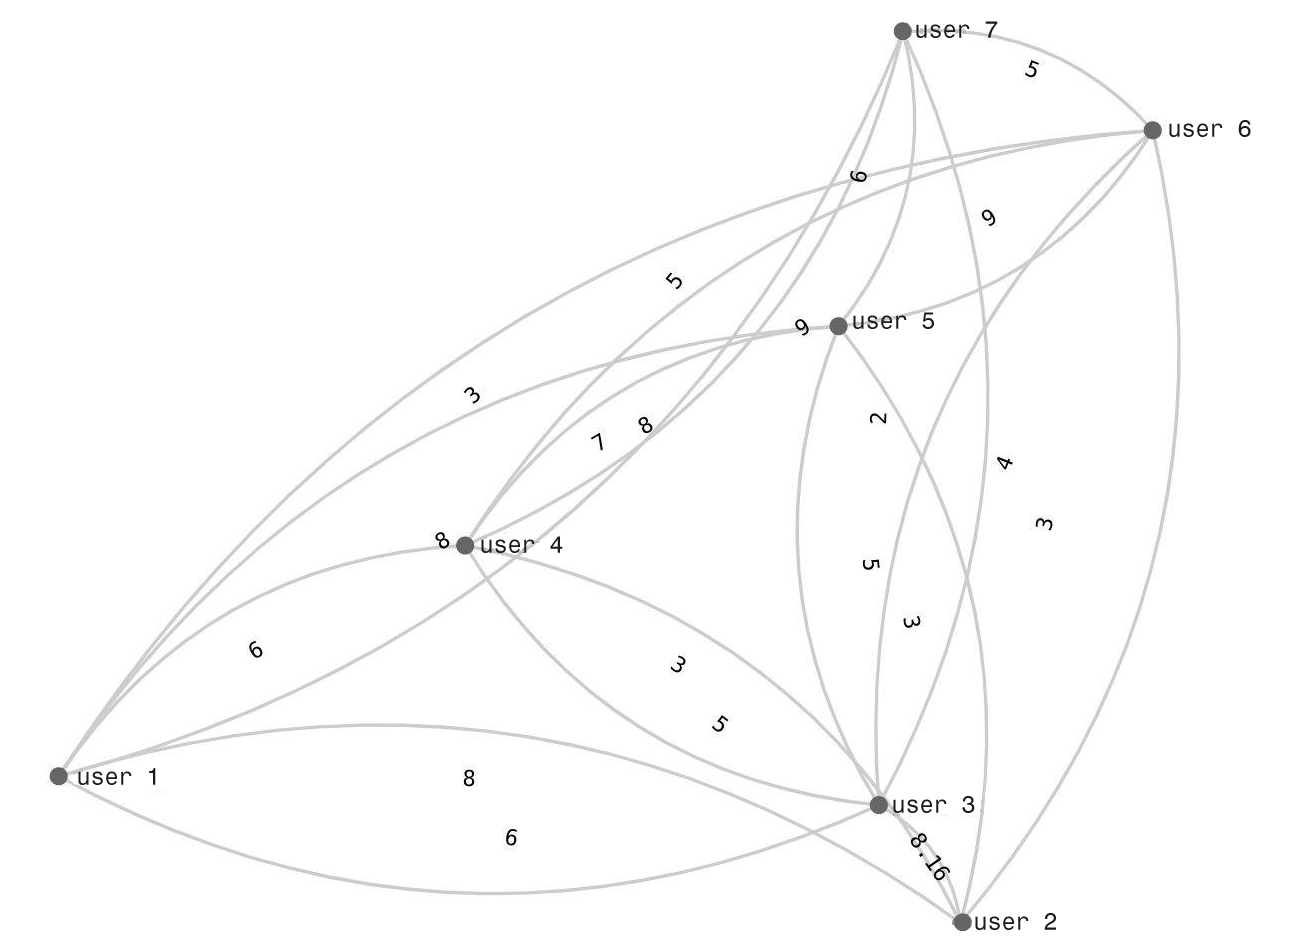
\includegraphics[width=12cm]{grafo.png}
\caption{Um grafo com 5 nós e 6 arestas.}
\label{fig:grafo}
\end{figure}

Quando a relação entre dois nós é simétrica, ou seja, a relação entre o nó $A$ e o nó $B$ é idêntica, diz-se que o grafo é \emph{não orientado}. Quando a relação entre dois nós é assimétrica, portanto, $A$ tem uma relação com $B$, mas essa relação não equivale a $B$ para $A$, tem-se um \emph{dígrafo} ou um \emph{grafo orientado}.

Este trabalho utiliza o grafo não orientado pois este bem representa as relações de amizade recíprocas. Tal decisão é tomada pois, quando da sugestão de um novo contato, ambos vão ser apresentados reciprocamente, estabelecendo, portanto, uma relação mútua de interação.

Diversas áreas da ciência, desde a biologia à linguística, utilizam grafos para representar dados. A representação de objetos e suas relações é uma ferramenta frequente em várias pesquisas.

Na ciência da computação, o grafo é a uma estrutura de dados amplamente frequente e existem centenas de problemas computacionais definidos com o seu uso \cite{Cormen2009}. Um caso tradicional com solução utilizando grafos é a do caixeiro viajante. Neste problema, os nós do grafo são as localidades e as arestas têm o peso equivalente à distância entre as cidades. \citep{Dijkstra1959}, propôs o primeiro algoritmo para encontrar o caminho mais curto entre dois nós de um grafo. O algoritmo encontra um caminho curto, mas não necessariamente o mais curto. Vários trabalhos são realizados ainda hoje na busca pelo caminho mais curto em um grafo. Muitos desses trabalhos são baseados no algoritmo de Dijkstra.

Como estrutura de dados computacionais, existem várias modelagens conhecidas para representação de um grafo. \citep{Cormen2009}, cita duas formas fundamentais:

\begin{itemize}
\item A lista de adjacência
\item A matriz de adjacência
\end{itemize}

\begin{figure}[!htb]
\centering
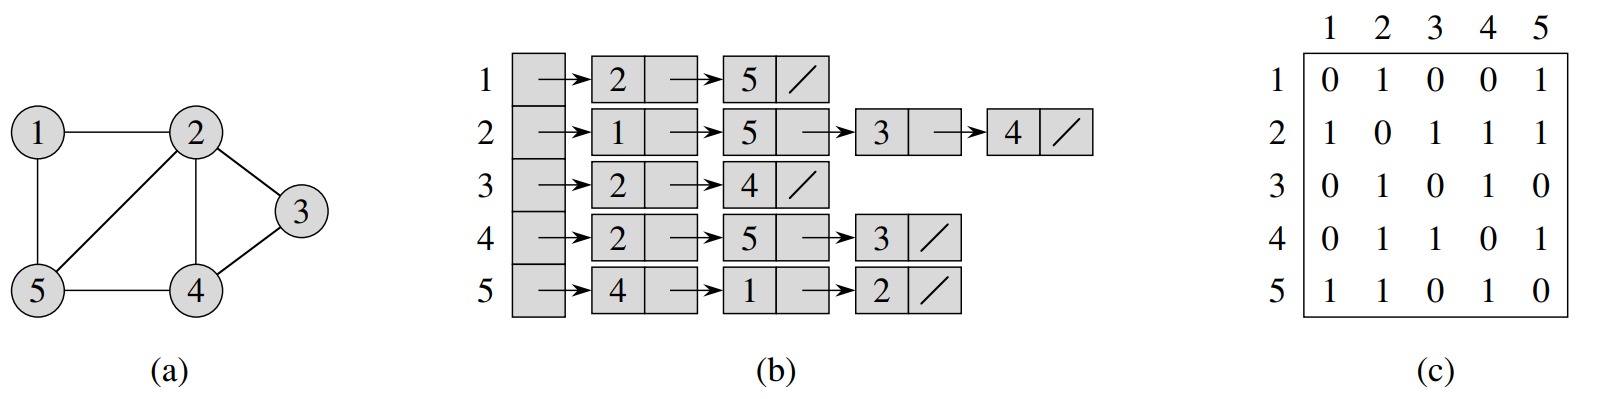
\includegraphics[width=16cm]{represent_grafo.png}
\caption{Duas representações de um grafo não direcionado. (\textbf{a}) Um grafo G com cinco nós e sete arestas. (\textbf{b}) A representação de uma lista de adjacência de G. (\textbf{c}) A representação de uma matriz de adjacência. Fonte: \cite{Cormen2009}, tradução dos autores.}
\label{fig:represent_grafo}
\end{figure}


\begin{figure}[!htb]
\centering
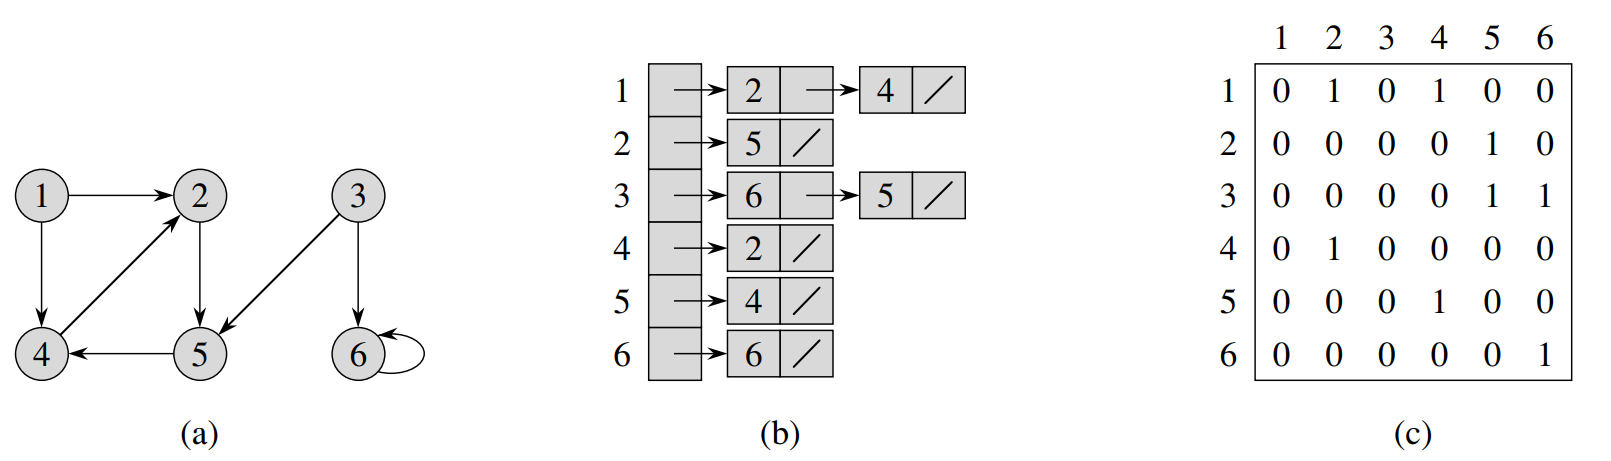
\includegraphics[width=16cm]{represent_grafo_ND.png}
\caption{Duas representações de um grafo direcionado. (\textbf{a}) Um grafo G com seis nós e oito arestas. (\textbf{b}) A representação de uma lista de adjacência de G. (\textbf{c}) A representação de uma matriz de adjacência. Fonte: \cite{Cormen2009}, tradução dos autores.}
\label{fig:represent_grafo_ND}
\end{figure}

\FloatBarrier

A Figura \ref{fig:represent_grafo}, ilustra um grafo $G$ como um diagrama, como uma lista de adjacência e como uma matriz de adjacência. A implementação computacional de um grafo pode ser a partir de uma lista de adjacência. Desse modo Um grafo $G = (N, E)$ consiste de uma lista de listas de nós, uma lista para cada nó em N. Para cada nó em G, tem-se uma lista dos nós vizinhos. Essa lista também pode conter somente um ponteiro para os nós vizinhos. Normalmente é suficiente armazenar os nós vizinhos em ordem arbitrária pois será o peso da aresta que determinará uma hierarquia entre os nós vizinhos, não a ordem pela qual eles foram adicionados nem qualquer outro atributo.
		% proposta
%\chapter{Fundamentação Teórica}
\label{cap:fund}

% figuras estão no subdiretório "figuras/" dentro deste capítulo
\graphicspath{\currfiledir/figuras/}

Nesta parte, há a exposição das definições e histórico de redes sociais, algoritmos de recomendação e as definições matemáticas e computacionais de grafo. Esses três itens relacionam-se intrinsicamente com este trabalho, por isso, buscamos esclarecê-los o suficiente neste capítulo de maneira que as relações destes tópicos com o objetivo geral estejam fundamentadas.


\section{Redes Sociais}

% \begin{itemize}
% \item Histórico de redes sociais
% \item Tipos de redes sociais
% \item Redes parecidas com nosso trabalho
% \item Análises de tempo despendido em redes sociais.
% \end{itemize}

Desde a invenção da internet em 1991, mais e mais aplicações vem sendo criadas para facilitar e estimular os relacionamentos virtuais. As redes sociais virtuais tiveram início em 1997 com o site \emph{Six Degrees}, \citep{terrel17}. \emph{Six Degrees} é nomeado em referência ao estudo de \cite{milgram67}, que teorizava que são necessários seis laços de amizade para que quaisquer pessoas estejam conectadas. \emph{Six Degrees} teve seu fim em 2001, mas iniciou o processo de popularização das redes sociais e é considerado a primeira rede social pois permitia que as pessoas criassem seus perfis individuais e adicionar outros contatos à sua rede. Teve 3,5 milhões de usuários no seu auge.

Entre as precursoras está também a rede especializada em relacionamentos profissionais, \emph{LinkedIn}. Foi criada no final de 2002 e tem, desde então, seu objetivo principal em criar conexões entre profissionais, estudantes e corporações. O \emph{LinkedIn} é, ainda hoje, a rede mais popular neste nicho com mais de 500 milhões de usuários.

A rede mais popular atualmente, segundo \cite{lua19}, é o Facebook com 2,23 milhões de usuários ativos mensalmente. O Facebook foi criado em 2004 como uma rede específica para estudantes da Universidade de Harvard. Em 2006 foi aberta ao público e em 2008 já era a rede social mais visitada do mundo.

Há também redes especializadas em outros tipos de conexão ou outras maneiras de publicar conteúdo. O YouTube é uma rede social especializada na divulgação de vídeos criados pelos usuários. O Twitter, distingue-se das outras redes por iniciar suas atividades permitindo apenas a publicação de textos com, no máximo, 140 caracteres. Este limite foi dobrado posteriormente, mas o foco ainda mantém-se em pequenas postagens.

Por fim, há as redes especializadas em relacionamentos românticos. O Tinder, o Happn e o OKCupid são exemplos de redes sociais direcionadas à criação de relacionamentos íntimos entre os usuários. O sistema desenvolvido neste trabalho enquadra-se nesta categoria pois tem o objetivo de colocar usuários em contato com pessoas desconhecidas que têm potencial para formarem amizades ou até mesmo casais.

No Brasil, 66\% da população tem acesso à internet segundo \cite{wearesocial18}. Dentre os usuários da internet 93\% são ativos em alguma rede social.
Segundo \cite{wearesocial18}, o brasileiro despende, em média, 3h39min por dia em alguma rede social. Este tempo é passado em contato com informações e pessoas de várias culturas diferentes. Muitas vezes as interações despertam sentimentos indesejados e a informação divulgada não é completamente conexa à realidade.

Por essa razão, mais e mais redes sociais oferecem a oportunidade, muitas vezes compulsoriamente, do usuário ser exposto somente à pessoas e conteúdos que tenham afinidade com seu perfil. Na busca por uma experiência agradável, as sugestões de conteúdo e contatos vão ao encontro da necessidade do ser humano de se socializar. E participar de uma rede social, seja ela física ou virtual, faz parte das necessidades básicas apontadas por \cite{Maslow1943}, ao definir uma hierarquia para as necessidades básicas do ser humano.

De uma maneira ou de outra, todas as redes sociais tem seu foco no conteúdo gerado pelos usuários. Porém, grande parte da monetização empregada refere-se à divulgação de peças publicitárias pagas por empresas particulares e públicas. Dentro deste escopo, são utilizados algoritmos que tomam em conta os interesses dos usuários para fazer sugestões de conteúdo publicitário. Há vários métodos para relacionar os dados produzidos pelos usuários para gerar sugestões, sejam elas de conteúdo, publicidade ou novos contatos.

%=====================================================

\section{Algoritmos de Recomendação}

% \begin{itemize}
% \item Como sugerir novos contatos.
% \item Como as outras redes fazem isso.
% 
% \end{itemize}


Quando um usuário acessa um sistema qualquer que lhe oferece itens, por exemplo, livros, um sistema de recomendação pode lhe proporcionar a conveniência de sugerir-lhe um livro mais adequado para o seu gosto quando a quantidade de opções disponíveis é opressivamente vasta, diz \cite{Ricci2010}.

Esses itens, são quaisquer coisas que podem ser sugeridas ao usuário, sejam produtos, serviços, notícias, publicidade, ou, no caso deste trabalho, outros usuários com potencial para tornarem-se amizades.

Para \cite{Ricci2010}, a forma mais simples de um sistema de recomendação é uma lista com itens ordenados pela similaridade com o usuário que receberá a recomendação. Os sistemas de sugestão analisam vários tipos de dados por diversos métodos diferentes para encontrar os itens mais adequados para cada usuário. De acordo com \cite{Ricci2010}, os primeiros algoritmos de recomendação utilizavam dados gerados por recomendações feitas pela comunidade de usuários. Esse método comparava gostos similares entre os usuários e recomendava itens ainda não consumidos por alguns usuários. A este método dá-se o nome de Filtragem Colaborativa \citep{goldberg92}.

Desde os anos 1990, a perseguição por sistemas de recomendações cada vez mais eficientes impulsionou o surgimento do Prêmio Netflix em 2006, \citep{netflix}. Neste concurso, a empresa Netflix propôs pagar um prêmio de US\$1.000.000 para quem elaborasse um sistema que pudesse melhorar em, pelo menos, 10\% a acurácia do sistema que estava em uso à época. O time \emph{BellKor's Pragmatic Chaos}, venceu a disputa empregando diversos algoritmos e métodos de classificação mesclados em um mesmo sistema, \citep{Bell}. 

Entre as possibilidades de métodos e algoritmos que podem ser empregados em um sistema de recomendação, podemos ressaltar, baseados no texto de \cite{Recommendation}, as seguintes:

\begin{itemize}
\item Filtragem colaborativa
\item Filtragem baseada em conteúdo
\item Recomendação baseada em conhecimento
\end{itemize}

A filtragem colaborativa, como já mencionado, leva em conta as preferências já informadas pelos usuários para compará-las e sugerir novas possibilidades de itens. Tem a tendência de sugerir itens que já são apreciados por usuários que, de alguma maneira, já se relacionam, seja por interesses definidos, grupos específicos ou até mesmo por parentesco.

A filtragem baseada em conteúdo toma por verdadeira a afirmação de que os usuários que já demonstraram interesse por um tópico somente serão agradados por tópicos semelhantes e não podem ser instigados por assuntos fora do escopo do que já foi definido como interesse inicialmente. Dessa maneira, o sistema considera de que um usuário que declarou interesse por filmes deve receber sugestões de itens relacionados a este tema. É claro que este método tem a fraqueza de não sugerir novos assuntos que, potencialmente, despertariam o interesse do usuário.

Finalmente, a recomendação baseada em conhecimento,  que toma em conta regras de restrições de interesse definidas no sistema e os aplica à lista de itens disponíveis. Desse modo, os itens são sugeridos a partir do resultado da filtragem realizada a partir das regras definidas. A definição de tais regras passa por análises semânticas do conteúdo disponível no sistema que diga respeito ao usuário. O sistema desenvolvido neste trabalho assemelha-se a uma recomendação baseada em conhecimento no sentido de que a regra definida para relacionar os itens será uma equação determinística que calcula um valor de proximidade entre dois itens.

Os vários métodos de recomendação tem sua acurácia diretamente influenciada pela quantidade de informação disponível sobre os usuários ou gerada pelos usuários. Quanto maior a quantidade de informação disponível, maior a acurácia e, em linhas gerais, menor a performance do sistema, uma vez que o tempo de processamento da informação é incrementado. Por essa razão, boas soluções são baseadas em aprendizado de máquina e inteligência artificial. O emprego dessas tecnologias tem o objetivo de melhorar a performance e a acurácia das sugestões.

%=====================================================

\section{Grafo}
% \begin{itemize}
% \item O que é grafo - \emph{Fonte básica de definição de grafo LIVRO??}
% \item Quantos tipos de grafo existem.
% \item Aplicações comuns de grafo
% \item Algoritmos que usam grafos
% \end{itemize}

O conceito matemático de grafo parte de abstrações de situações da vida real onde objetos ou pessoas representadas por pontos e suas conexões e interações são representadas por linhas \cite{Bondy08}. Numa rede social, as pessoas são esses pontos, que convencionalmente são chamados de nós, e suas relações com outras pessoas são representadas por linhas, chamadas de arestas. Um grafo é uma tripla ordenada $G=(N(G), A(G), \psi _{G})$, que consiste de um conjunto não vazio $N(G)$ de nós, um conjunto $A(G)$, diferente de $N(G)$, de arestas, e uma \emph{função de incidência} $\psi_{G}$ que associa a cada nó de $G$ um par não ordenado de nós de $G$. Se $e$ é uma aresta de $G$ e $u$ e $v$ são arestas de tal modo que $\psi_{G}(e) = un$, então $e$ é dito que \emph{une} $u$ e $n$ \cite{Bondy08}.

\emph{Exemplo}

\begin{equation}
G=(N(G), A(G), \psi _{G})
\label{eq:grafo}
\end{equation}

\emph{onde}

\begin{equation}
N(G)={n_{1}, n_{2}, n_{3}, n_{4}, n_{5}}
\label{eq:grafo2}
\end{equation}

\emph{e $\psi_{G}$ é definido por}

\begin{equation}
\begin{split}
\psi_{G}(a_{1}) = n_{1}n_{2}, \psi_{G}(a_{2} = n_{2}n_{3}, \psi_{G}(a_{3}) = n_{3}n_{3}, \psi_{G}(a_{4}) = n_{2}n_{4} \\
\psi_{G}(a_{5}) = n_{2}n_{4}, \psi_{G}(a_{6} = n_{4}n_{5}, \psi_{G}(n_{8}) = n_{2}n_{5}, \psi_{G}(a_{4}) = n_{2}n_{4}
\label{eq:grafo3}
\end{split}
\end{equation}

Grafos têm este nome pois podem ser representadas graficamente, segundo \cite{Bondy08}. A Figura \ref{fig:grafo}, é um diagrama que representa um grafo com 5 nós e 6 arestas. Nesta Figura, os nós têm identificação - letras - e as arestas tem um \emph{peso}. O peso das arestas pode ser usado para representar a força da ligação entre os nós ou até mesmo a distância entre os nós. A convenção tomada neste caso depende do contexto e da aplicação do grafo.

\begin{figure}[!htb]
\centering
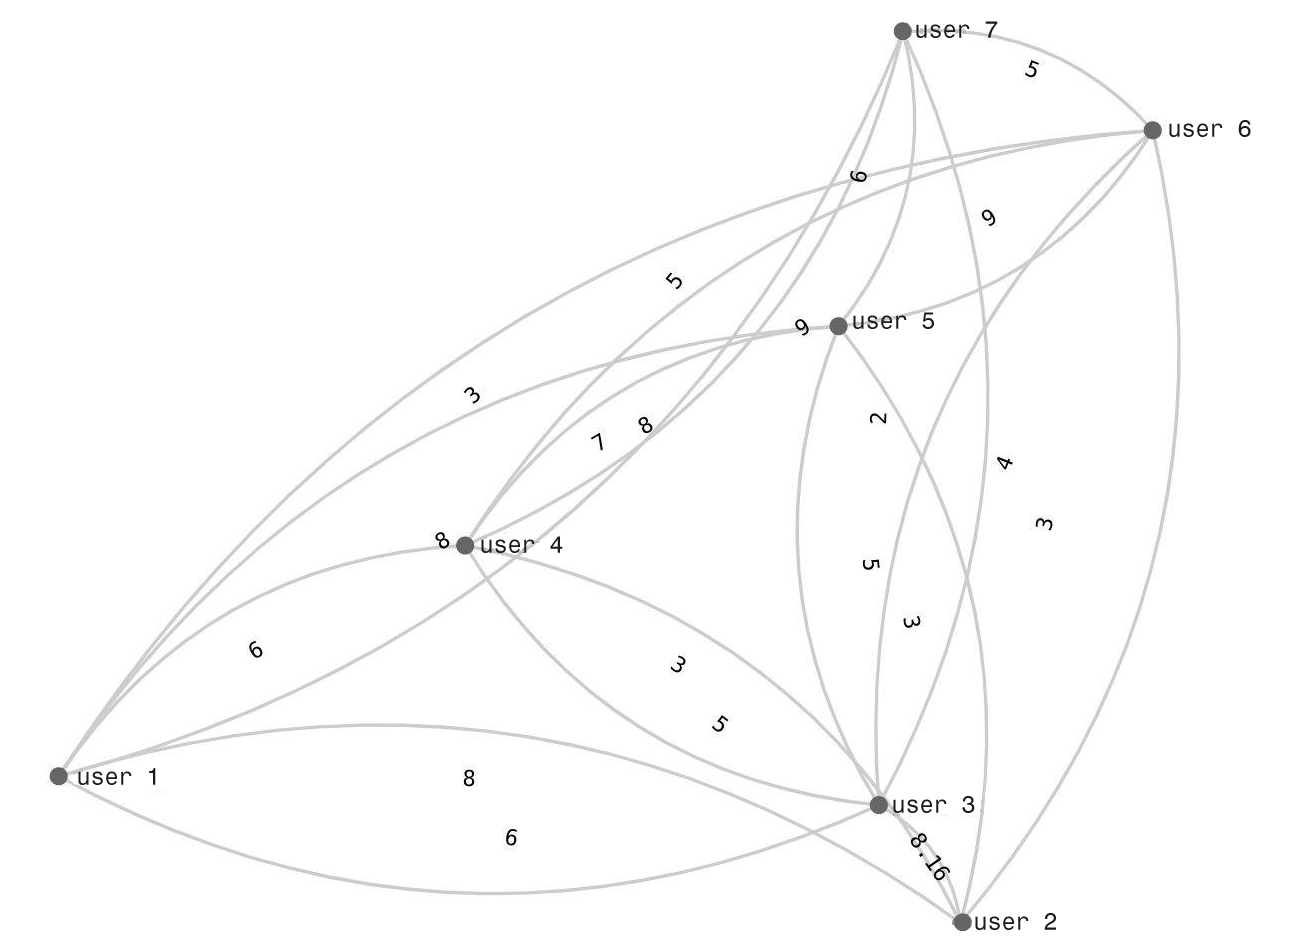
\includegraphics[width=12cm]{grafo.png}
\caption{Um grafo com 5 nós e 6 arestas.}
\label{fig:grafo}
\end{figure}

Quando a relação entre dois nós é simétrica, ou seja, a relação entre o nó $A$ e o nó $B$ é idêntica, diz-se que o grafo é \emph{não orientado}. Quando a relação entre dois nós é assimétrica, portanto, $A$ tem uma relação com $B$, mas essa relação não equivale a $B$ para $A$, tem-se um \emph{dígrafo} ou um \emph{grafo orientado}.

Este trabalho utiliza o grafo não orientado pois este bem representa as relações de amizade recíprocas. Tal decisão é tomada pois, quando da sugestão de um novo contato, ambos vão ser apresentados reciprocamente, estabelecendo, portanto, uma relação mútua de interação.

Diversas áreas da ciência, desde a biologia à linguística, utilizam grafos para representar dados. A representação de objetos e suas relações é uma ferramenta frequente em várias pesquisas.

Na ciência da computação, o grafo é a uma estrutura de dados amplamente frequente e existem centenas de problemas computacionais definidos com o seu uso \cite{Cormen2009}. Um caso tradicional com solução utilizando grafos é a do caixeiro viajante. Neste problema, os nós do grafo são as localidades e as arestas têm o peso equivalente à distância entre as cidades. \citep{Dijkstra1959}, propôs o primeiro algoritmo para encontrar o caminho mais curto entre dois nós de um grafo. O algoritmo encontra um caminho curto, mas não necessariamente o mais curto. Vários trabalhos são realizados ainda hoje na busca pelo caminho mais curto em um grafo. Muitos desses trabalhos são baseados no algoritmo de Dijkstra.

Como estrutura de dados computacionais, existem várias modelagens conhecidas para representação de um grafo. \citep{Cormen2009}, cita duas formas fundamentais:

\begin{itemize}
\item A lista de adjacência
\item A matriz de adjacência
\end{itemize}

\begin{figure}[!htb]
\centering
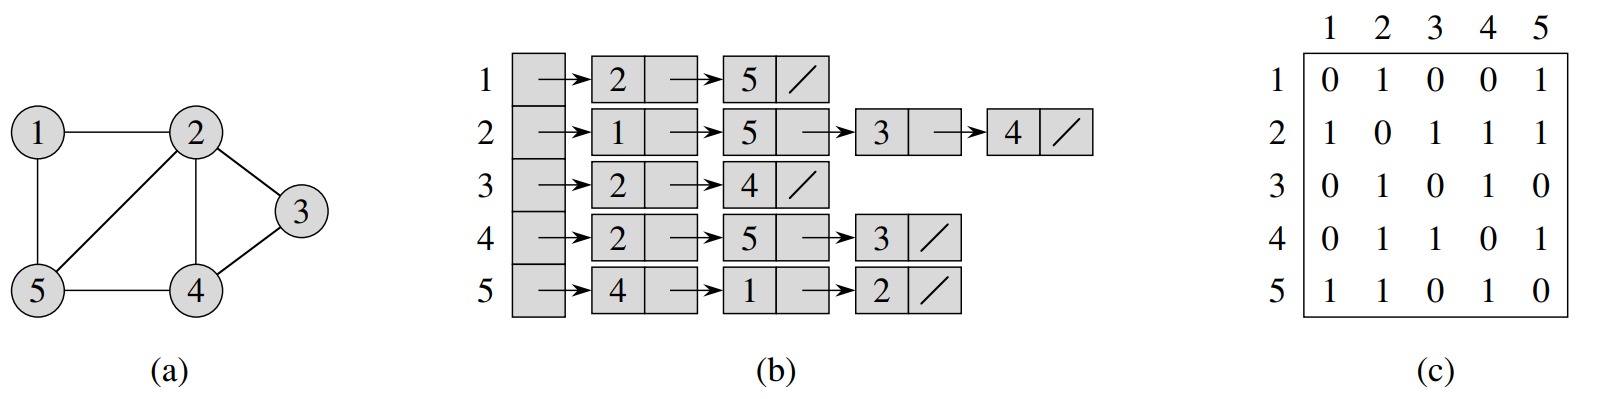
\includegraphics[width=16cm]{represent_grafo.png}
\caption{Duas representações de um grafo não direcionado. (\textbf{a}) Um grafo G com cinco nós e sete arestas. (\textbf{b}) A representação de uma lista de adjacência de G. (\textbf{c}) A representação de uma matriz de adjacência. Fonte: \cite{Cormen2009}, tradução dos autores.}
\label{fig:represent_grafo}
\end{figure}


\begin{figure}[!htb]
\centering
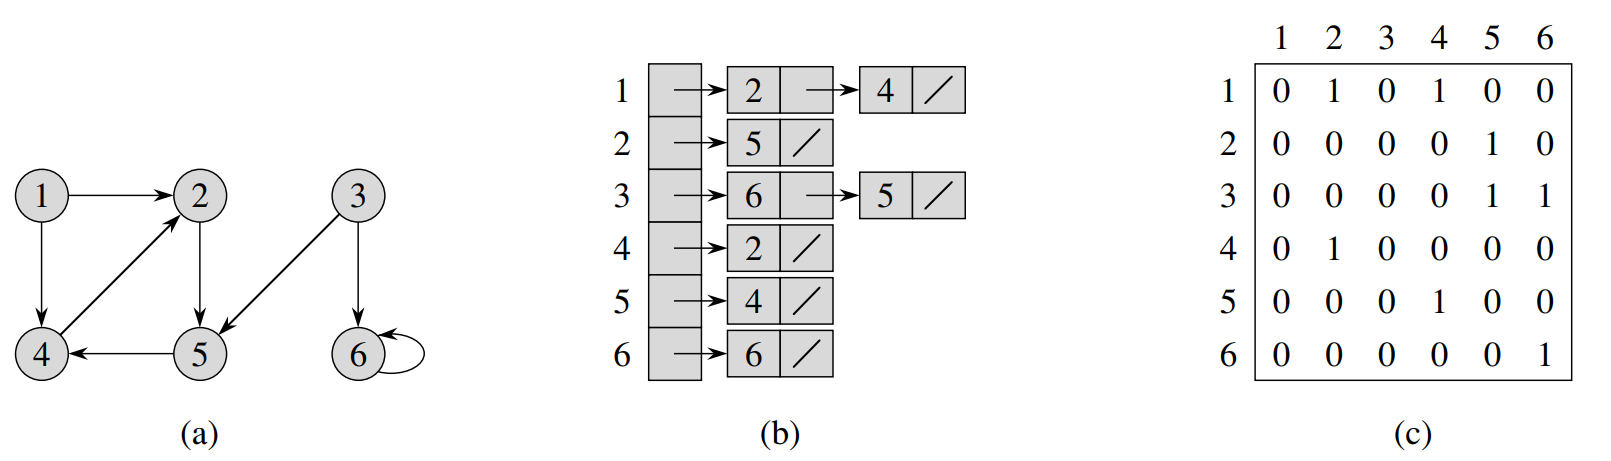
\includegraphics[width=16cm]{represent_grafo_ND.png}
\caption{Duas representações de um grafo direcionado. (\textbf{a}) Um grafo G com seis nós e oito arestas. (\textbf{b}) A representação de uma lista de adjacência de G. (\textbf{c}) A representação de uma matriz de adjacência. Fonte: \cite{Cormen2009}, tradução dos autores.}
\label{fig:represent_grafo_ND}
\end{figure}

\FloatBarrier

A Figura \ref{fig:represent_grafo}, ilustra um grafo $G$ como um diagrama, como uma lista de adjacência e como uma matriz de adjacência. A implementação computacional de um grafo pode ser a partir de uma lista de adjacência. Desse modo Um grafo $G = (N, E)$ consiste de uma lista de listas de nós, uma lista para cada nó em N. Para cada nó em G, tem-se uma lista dos nós vizinhos. Essa lista também pode conter somente um ponteiro para os nós vizinhos. Normalmente é suficiente armazenar os nós vizinhos em ordem arbitrária pois será o peso da aresta que determinará uma hierarquia entre os nós vizinhos, não a ordem pela qual eles foram adicionados nem qualquer outro atributo.
		% experimentação e validação
%\chapter{Fundamentação Teórica}
\label{cap:fund}

% figuras estão no subdiretório "figuras/" dentro deste capítulo
\graphicspath{\currfiledir/figuras/}

Nesta parte, há a exposição das definições e histórico de redes sociais, algoritmos de recomendação e as definições matemáticas e computacionais de grafo. Esses três itens relacionam-se intrinsicamente com este trabalho, por isso, buscamos esclarecê-los o suficiente neste capítulo de maneira que as relações destes tópicos com o objetivo geral estejam fundamentadas.


\section{Redes Sociais}

% \begin{itemize}
% \item Histórico de redes sociais
% \item Tipos de redes sociais
% \item Redes parecidas com nosso trabalho
% \item Análises de tempo despendido em redes sociais.
% \end{itemize}

Desde a invenção da internet em 1991, mais e mais aplicações vem sendo criadas para facilitar e estimular os relacionamentos virtuais. As redes sociais virtuais tiveram início em 1997 com o site \emph{Six Degrees}, \citep{terrel17}. \emph{Six Degrees} é nomeado em referência ao estudo de \cite{milgram67}, que teorizava que são necessários seis laços de amizade para que quaisquer pessoas estejam conectadas. \emph{Six Degrees} teve seu fim em 2001, mas iniciou o processo de popularização das redes sociais e é considerado a primeira rede social pois permitia que as pessoas criassem seus perfis individuais e adicionar outros contatos à sua rede. Teve 3,5 milhões de usuários no seu auge.

Entre as precursoras está também a rede especializada em relacionamentos profissionais, \emph{LinkedIn}. Foi criada no final de 2002 e tem, desde então, seu objetivo principal em criar conexões entre profissionais, estudantes e corporações. O \emph{LinkedIn} é, ainda hoje, a rede mais popular neste nicho com mais de 500 milhões de usuários.

A rede mais popular atualmente, segundo \cite{lua19}, é o Facebook com 2,23 milhões de usuários ativos mensalmente. O Facebook foi criado em 2004 como uma rede específica para estudantes da Universidade de Harvard. Em 2006 foi aberta ao público e em 2008 já era a rede social mais visitada do mundo.

Há também redes especializadas em outros tipos de conexão ou outras maneiras de publicar conteúdo. O YouTube é uma rede social especializada na divulgação de vídeos criados pelos usuários. O Twitter, distingue-se das outras redes por iniciar suas atividades permitindo apenas a publicação de textos com, no máximo, 140 caracteres. Este limite foi dobrado posteriormente, mas o foco ainda mantém-se em pequenas postagens.

Por fim, há as redes especializadas em relacionamentos românticos. O Tinder, o Happn e o OKCupid são exemplos de redes sociais direcionadas à criação de relacionamentos íntimos entre os usuários. O sistema desenvolvido neste trabalho enquadra-se nesta categoria pois tem o objetivo de colocar usuários em contato com pessoas desconhecidas que têm potencial para formarem amizades ou até mesmo casais.

No Brasil, 66\% da população tem acesso à internet segundo \cite{wearesocial18}. Dentre os usuários da internet 93\% são ativos em alguma rede social.
Segundo \cite{wearesocial18}, o brasileiro despende, em média, 3h39min por dia em alguma rede social. Este tempo é passado em contato com informações e pessoas de várias culturas diferentes. Muitas vezes as interações despertam sentimentos indesejados e a informação divulgada não é completamente conexa à realidade.

Por essa razão, mais e mais redes sociais oferecem a oportunidade, muitas vezes compulsoriamente, do usuário ser exposto somente à pessoas e conteúdos que tenham afinidade com seu perfil. Na busca por uma experiência agradável, as sugestões de conteúdo e contatos vão ao encontro da necessidade do ser humano de se socializar. E participar de uma rede social, seja ela física ou virtual, faz parte das necessidades básicas apontadas por \cite{Maslow1943}, ao definir uma hierarquia para as necessidades básicas do ser humano.

De uma maneira ou de outra, todas as redes sociais tem seu foco no conteúdo gerado pelos usuários. Porém, grande parte da monetização empregada refere-se à divulgação de peças publicitárias pagas por empresas particulares e públicas. Dentro deste escopo, são utilizados algoritmos que tomam em conta os interesses dos usuários para fazer sugestões de conteúdo publicitário. Há vários métodos para relacionar os dados produzidos pelos usuários para gerar sugestões, sejam elas de conteúdo, publicidade ou novos contatos.

%=====================================================

\section{Algoritmos de Recomendação}

% \begin{itemize}
% \item Como sugerir novos contatos.
% \item Como as outras redes fazem isso.
% 
% \end{itemize}


Quando um usuário acessa um sistema qualquer que lhe oferece itens, por exemplo, livros, um sistema de recomendação pode lhe proporcionar a conveniência de sugerir-lhe um livro mais adequado para o seu gosto quando a quantidade de opções disponíveis é opressivamente vasta, diz \cite{Ricci2010}.

Esses itens, são quaisquer coisas que podem ser sugeridas ao usuário, sejam produtos, serviços, notícias, publicidade, ou, no caso deste trabalho, outros usuários com potencial para tornarem-se amizades.

Para \cite{Ricci2010}, a forma mais simples de um sistema de recomendação é uma lista com itens ordenados pela similaridade com o usuário que receberá a recomendação. Os sistemas de sugestão analisam vários tipos de dados por diversos métodos diferentes para encontrar os itens mais adequados para cada usuário. De acordo com \cite{Ricci2010}, os primeiros algoritmos de recomendação utilizavam dados gerados por recomendações feitas pela comunidade de usuários. Esse método comparava gostos similares entre os usuários e recomendava itens ainda não consumidos por alguns usuários. A este método dá-se o nome de Filtragem Colaborativa \citep{goldberg92}.

Desde os anos 1990, a perseguição por sistemas de recomendações cada vez mais eficientes impulsionou o surgimento do Prêmio Netflix em 2006, \citep{netflix}. Neste concurso, a empresa Netflix propôs pagar um prêmio de US\$1.000.000 para quem elaborasse um sistema que pudesse melhorar em, pelo menos, 10\% a acurácia do sistema que estava em uso à época. O time \emph{BellKor's Pragmatic Chaos}, venceu a disputa empregando diversos algoritmos e métodos de classificação mesclados em um mesmo sistema, \citep{Bell}. 

Entre as possibilidades de métodos e algoritmos que podem ser empregados em um sistema de recomendação, podemos ressaltar, baseados no texto de \cite{Recommendation}, as seguintes:

\begin{itemize}
\item Filtragem colaborativa
\item Filtragem baseada em conteúdo
\item Recomendação baseada em conhecimento
\end{itemize}

A filtragem colaborativa, como já mencionado, leva em conta as preferências já informadas pelos usuários para compará-las e sugerir novas possibilidades de itens. Tem a tendência de sugerir itens que já são apreciados por usuários que, de alguma maneira, já se relacionam, seja por interesses definidos, grupos específicos ou até mesmo por parentesco.

A filtragem baseada em conteúdo toma por verdadeira a afirmação de que os usuários que já demonstraram interesse por um tópico somente serão agradados por tópicos semelhantes e não podem ser instigados por assuntos fora do escopo do que já foi definido como interesse inicialmente. Dessa maneira, o sistema considera de que um usuário que declarou interesse por filmes deve receber sugestões de itens relacionados a este tema. É claro que este método tem a fraqueza de não sugerir novos assuntos que, potencialmente, despertariam o interesse do usuário.

Finalmente, a recomendação baseada em conhecimento,  que toma em conta regras de restrições de interesse definidas no sistema e os aplica à lista de itens disponíveis. Desse modo, os itens são sugeridos a partir do resultado da filtragem realizada a partir das regras definidas. A definição de tais regras passa por análises semânticas do conteúdo disponível no sistema que diga respeito ao usuário. O sistema desenvolvido neste trabalho assemelha-se a uma recomendação baseada em conhecimento no sentido de que a regra definida para relacionar os itens será uma equação determinística que calcula um valor de proximidade entre dois itens.

Os vários métodos de recomendação tem sua acurácia diretamente influenciada pela quantidade de informação disponível sobre os usuários ou gerada pelos usuários. Quanto maior a quantidade de informação disponível, maior a acurácia e, em linhas gerais, menor a performance do sistema, uma vez que o tempo de processamento da informação é incrementado. Por essa razão, boas soluções são baseadas em aprendizado de máquina e inteligência artificial. O emprego dessas tecnologias tem o objetivo de melhorar a performance e a acurácia das sugestões.

%=====================================================

\section{Grafo}
% \begin{itemize}
% \item O que é grafo - \emph{Fonte básica de definição de grafo LIVRO??}
% \item Quantos tipos de grafo existem.
% \item Aplicações comuns de grafo
% \item Algoritmos que usam grafos
% \end{itemize}

O conceito matemático de grafo parte de abstrações de situações da vida real onde objetos ou pessoas representadas por pontos e suas conexões e interações são representadas por linhas \cite{Bondy08}. Numa rede social, as pessoas são esses pontos, que convencionalmente são chamados de nós, e suas relações com outras pessoas são representadas por linhas, chamadas de arestas. Um grafo é uma tripla ordenada $G=(N(G), A(G), \psi _{G})$, que consiste de um conjunto não vazio $N(G)$ de nós, um conjunto $A(G)$, diferente de $N(G)$, de arestas, e uma \emph{função de incidência} $\psi_{G}$ que associa a cada nó de $G$ um par não ordenado de nós de $G$. Se $e$ é uma aresta de $G$ e $u$ e $v$ são arestas de tal modo que $\psi_{G}(e) = un$, então $e$ é dito que \emph{une} $u$ e $n$ \cite{Bondy08}.

\emph{Exemplo}

\begin{equation}
G=(N(G), A(G), \psi _{G})
\label{eq:grafo}
\end{equation}

\emph{onde}

\begin{equation}
N(G)={n_{1}, n_{2}, n_{3}, n_{4}, n_{5}}
\label{eq:grafo2}
\end{equation}

\emph{e $\psi_{G}$ é definido por}

\begin{equation}
\begin{split}
\psi_{G}(a_{1}) = n_{1}n_{2}, \psi_{G}(a_{2} = n_{2}n_{3}, \psi_{G}(a_{3}) = n_{3}n_{3}, \psi_{G}(a_{4}) = n_{2}n_{4} \\
\psi_{G}(a_{5}) = n_{2}n_{4}, \psi_{G}(a_{6} = n_{4}n_{5}, \psi_{G}(n_{8}) = n_{2}n_{5}, \psi_{G}(a_{4}) = n_{2}n_{4}
\label{eq:grafo3}
\end{split}
\end{equation}

Grafos têm este nome pois podem ser representadas graficamente, segundo \cite{Bondy08}. A Figura \ref{fig:grafo}, é um diagrama que representa um grafo com 5 nós e 6 arestas. Nesta Figura, os nós têm identificação - letras - e as arestas tem um \emph{peso}. O peso das arestas pode ser usado para representar a força da ligação entre os nós ou até mesmo a distância entre os nós. A convenção tomada neste caso depende do contexto e da aplicação do grafo.

\begin{figure}[!htb]
\centering
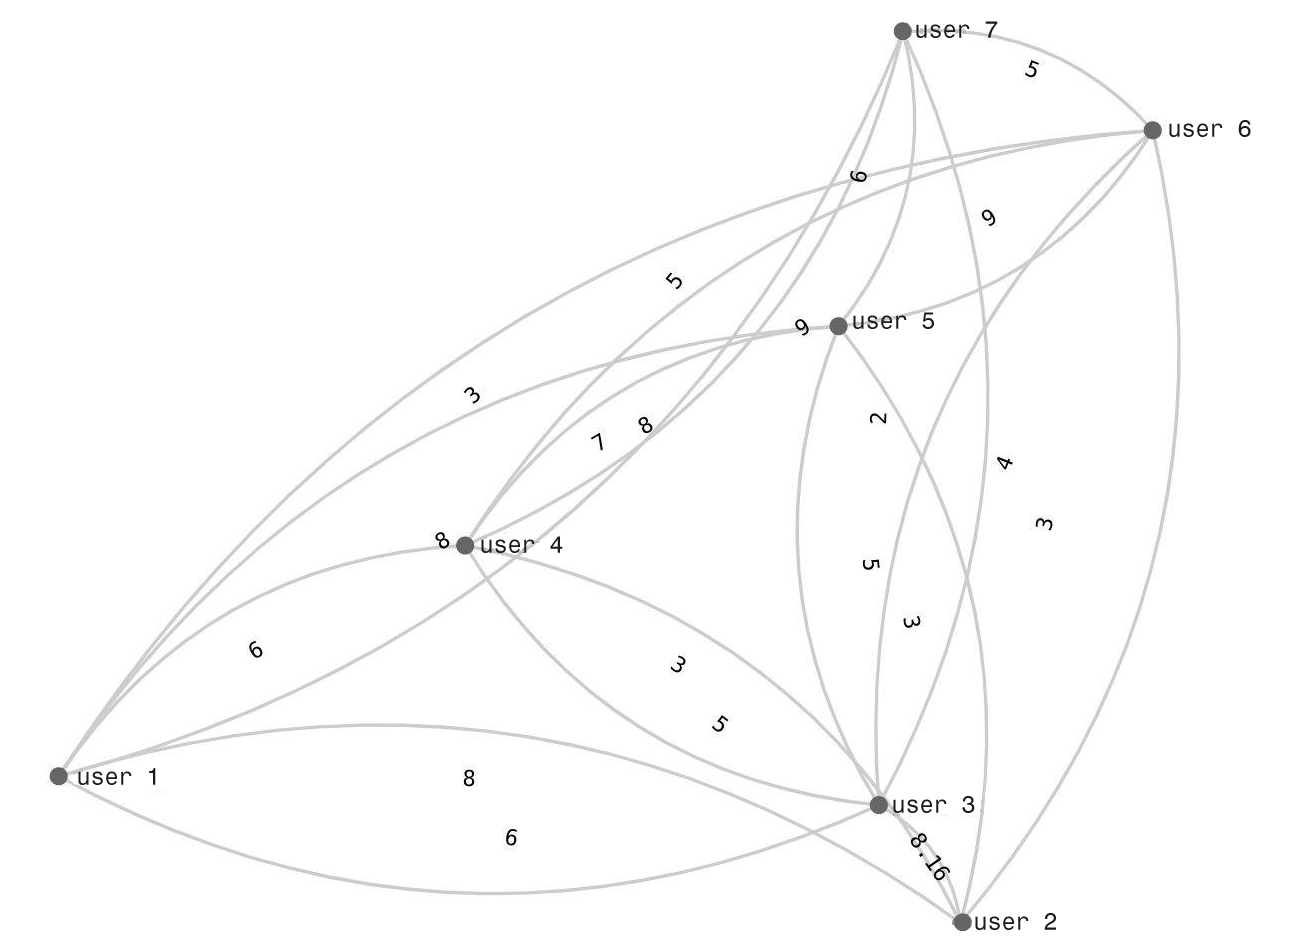
\includegraphics[width=12cm]{grafo.png}
\caption{Um grafo com 5 nós e 6 arestas.}
\label{fig:grafo}
\end{figure}

Quando a relação entre dois nós é simétrica, ou seja, a relação entre o nó $A$ e o nó $B$ é idêntica, diz-se que o grafo é \emph{não orientado}. Quando a relação entre dois nós é assimétrica, portanto, $A$ tem uma relação com $B$, mas essa relação não equivale a $B$ para $A$, tem-se um \emph{dígrafo} ou um \emph{grafo orientado}.

Este trabalho utiliza o grafo não orientado pois este bem representa as relações de amizade recíprocas. Tal decisão é tomada pois, quando da sugestão de um novo contato, ambos vão ser apresentados reciprocamente, estabelecendo, portanto, uma relação mútua de interação.

Diversas áreas da ciência, desde a biologia à linguística, utilizam grafos para representar dados. A representação de objetos e suas relações é uma ferramenta frequente em várias pesquisas.

Na ciência da computação, o grafo é a uma estrutura de dados amplamente frequente e existem centenas de problemas computacionais definidos com o seu uso \cite{Cormen2009}. Um caso tradicional com solução utilizando grafos é a do caixeiro viajante. Neste problema, os nós do grafo são as localidades e as arestas têm o peso equivalente à distância entre as cidades. \citep{Dijkstra1959}, propôs o primeiro algoritmo para encontrar o caminho mais curto entre dois nós de um grafo. O algoritmo encontra um caminho curto, mas não necessariamente o mais curto. Vários trabalhos são realizados ainda hoje na busca pelo caminho mais curto em um grafo. Muitos desses trabalhos são baseados no algoritmo de Dijkstra.

Como estrutura de dados computacionais, existem várias modelagens conhecidas para representação de um grafo. \citep{Cormen2009}, cita duas formas fundamentais:

\begin{itemize}
\item A lista de adjacência
\item A matriz de adjacência
\end{itemize}

\begin{figure}[!htb]
\centering
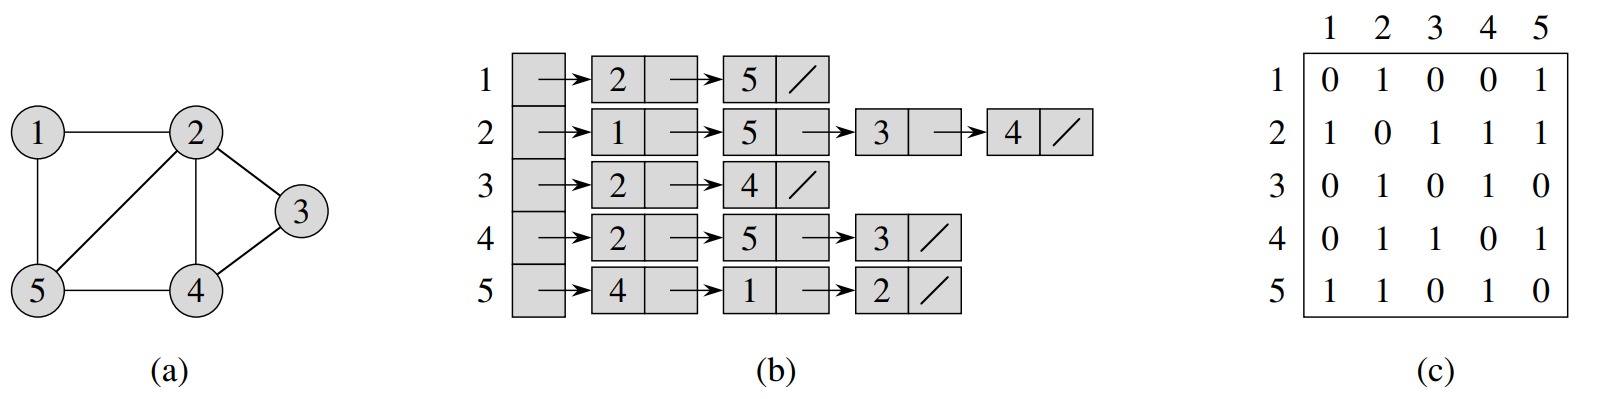
\includegraphics[width=16cm]{represent_grafo.png}
\caption{Duas representações de um grafo não direcionado. (\textbf{a}) Um grafo G com cinco nós e sete arestas. (\textbf{b}) A representação de uma lista de adjacência de G. (\textbf{c}) A representação de uma matriz de adjacência. Fonte: \cite{Cormen2009}, tradução dos autores.}
\label{fig:represent_grafo}
\end{figure}


\begin{figure}[!htb]
\centering
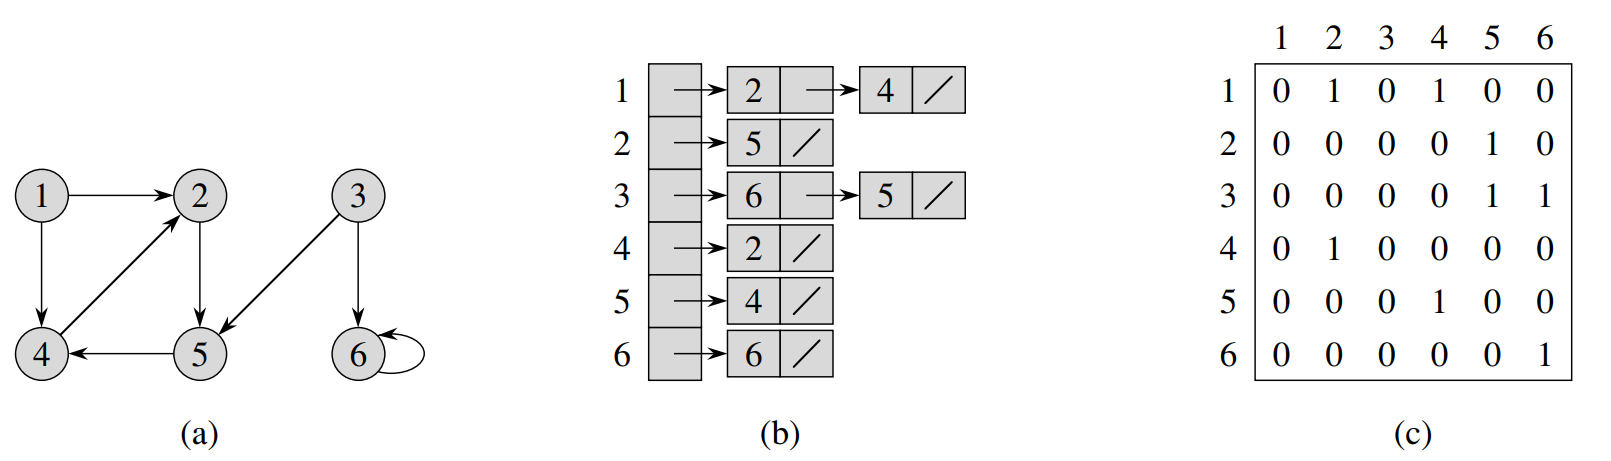
\includegraphics[width=16cm]{represent_grafo_ND.png}
\caption{Duas representações de um grafo direcionado. (\textbf{a}) Um grafo G com seis nós e oito arestas. (\textbf{b}) A representação de uma lista de adjacência de G. (\textbf{c}) A representação de uma matriz de adjacência. Fonte: \cite{Cormen2009}, tradução dos autores.}
\label{fig:represent_grafo_ND}
\end{figure}

\FloatBarrier

A Figura \ref{fig:represent_grafo}, ilustra um grafo $G$ como um diagrama, como uma lista de adjacência e como uma matriz de adjacência. A implementação computacional de um grafo pode ser a partir de uma lista de adjacência. Desse modo Um grafo $G = (N, E)$ consiste de uma lista de listas de nós, uma lista para cada nó em N. Para cada nó em G, tem-se uma lista dos nós vizinhos. Essa lista também pode conter somente um ponteiro para os nós vizinhos. Normalmente é suficiente armazenar os nós vizinhos em ordem arbitrária pois será o peso da aresta que determinará uma hierarquia entre os nós vizinhos, não a ordem pela qual eles foram adicionados nem qualquer outro atributo.
		% conclusão

%=====================================================

% Estilos de bibliografia recomendados (só descomentar um estilo!)
% Mais infos: https://pt.sharelatex.com/learn/Bibtex_bibliography_styles
\bibliographystyle{apalike-ptbr}	% [Maziero et al., 2006]
%\bibliographystyle{alpha}		% [Maz06]
%\bibliographystyle{plainnat}		% vide Google "LaTeX Natbib"
%\bibliographystyle{plain}		% [1] ordem alfabética
%\bibliographystyle{unsrt}		% [1] ordem de uso no texto

% no estilo "unsrt", evita que citações nos índices sejam consideradas
%\usepackage{notoccite}

% base de bibliografia (BibTeX)
\bibliography{referencias}
%\bibliography{file1, file2, file3} % se tiver mais de um arquivo BibTeX

%=====================================================

% inclusão de apêndices
\appendix

% inclusão de apêndice
\chapter{Fundamentação Teórica}
\label{cap:fund}

% figuras estão no subdiretório "figuras/" dentro deste capítulo
\graphicspath{\currfiledir/figuras/}

Nesta parte, há a exposição das definições e histórico de redes sociais, algoritmos de recomendação e as definições matemáticas e computacionais de grafo. Esses três itens relacionam-se intrinsicamente com este trabalho, por isso, buscamos esclarecê-los o suficiente neste capítulo de maneira que as relações destes tópicos com o objetivo geral estejam fundamentadas.


\section{Redes Sociais}

% \begin{itemize}
% \item Histórico de redes sociais
% \item Tipos de redes sociais
% \item Redes parecidas com nosso trabalho
% \item Análises de tempo despendido em redes sociais.
% \end{itemize}

Desde a invenção da internet em 1991, mais e mais aplicações vem sendo criadas para facilitar e estimular os relacionamentos virtuais. As redes sociais virtuais tiveram início em 1997 com o site \emph{Six Degrees}, \citep{terrel17}. \emph{Six Degrees} é nomeado em referência ao estudo de \cite{milgram67}, que teorizava que são necessários seis laços de amizade para que quaisquer pessoas estejam conectadas. \emph{Six Degrees} teve seu fim em 2001, mas iniciou o processo de popularização das redes sociais e é considerado a primeira rede social pois permitia que as pessoas criassem seus perfis individuais e adicionar outros contatos à sua rede. Teve 3,5 milhões de usuários no seu auge.

Entre as precursoras está também a rede especializada em relacionamentos profissionais, \emph{LinkedIn}. Foi criada no final de 2002 e tem, desde então, seu objetivo principal em criar conexões entre profissionais, estudantes e corporações. O \emph{LinkedIn} é, ainda hoje, a rede mais popular neste nicho com mais de 500 milhões de usuários.

A rede mais popular atualmente, segundo \cite{lua19}, é o Facebook com 2,23 milhões de usuários ativos mensalmente. O Facebook foi criado em 2004 como uma rede específica para estudantes da Universidade de Harvard. Em 2006 foi aberta ao público e em 2008 já era a rede social mais visitada do mundo.

Há também redes especializadas em outros tipos de conexão ou outras maneiras de publicar conteúdo. O YouTube é uma rede social especializada na divulgação de vídeos criados pelos usuários. O Twitter, distingue-se das outras redes por iniciar suas atividades permitindo apenas a publicação de textos com, no máximo, 140 caracteres. Este limite foi dobrado posteriormente, mas o foco ainda mantém-se em pequenas postagens.

Por fim, há as redes especializadas em relacionamentos românticos. O Tinder, o Happn e o OKCupid são exemplos de redes sociais direcionadas à criação de relacionamentos íntimos entre os usuários. O sistema desenvolvido neste trabalho enquadra-se nesta categoria pois tem o objetivo de colocar usuários em contato com pessoas desconhecidas que têm potencial para formarem amizades ou até mesmo casais.

No Brasil, 66\% da população tem acesso à internet segundo \cite{wearesocial18}. Dentre os usuários da internet 93\% são ativos em alguma rede social.
Segundo \cite{wearesocial18}, o brasileiro despende, em média, 3h39min por dia em alguma rede social. Este tempo é passado em contato com informações e pessoas de várias culturas diferentes. Muitas vezes as interações despertam sentimentos indesejados e a informação divulgada não é completamente conexa à realidade.

Por essa razão, mais e mais redes sociais oferecem a oportunidade, muitas vezes compulsoriamente, do usuário ser exposto somente à pessoas e conteúdos que tenham afinidade com seu perfil. Na busca por uma experiência agradável, as sugestões de conteúdo e contatos vão ao encontro da necessidade do ser humano de se socializar. E participar de uma rede social, seja ela física ou virtual, faz parte das necessidades básicas apontadas por \cite{Maslow1943}, ao definir uma hierarquia para as necessidades básicas do ser humano.

De uma maneira ou de outra, todas as redes sociais tem seu foco no conteúdo gerado pelos usuários. Porém, grande parte da monetização empregada refere-se à divulgação de peças publicitárias pagas por empresas particulares e públicas. Dentro deste escopo, são utilizados algoritmos que tomam em conta os interesses dos usuários para fazer sugestões de conteúdo publicitário. Há vários métodos para relacionar os dados produzidos pelos usuários para gerar sugestões, sejam elas de conteúdo, publicidade ou novos contatos.

%=====================================================

\section{Algoritmos de Recomendação}

% \begin{itemize}
% \item Como sugerir novos contatos.
% \item Como as outras redes fazem isso.
% 
% \end{itemize}


Quando um usuário acessa um sistema qualquer que lhe oferece itens, por exemplo, livros, um sistema de recomendação pode lhe proporcionar a conveniência de sugerir-lhe um livro mais adequado para o seu gosto quando a quantidade de opções disponíveis é opressivamente vasta, diz \cite{Ricci2010}.

Esses itens, são quaisquer coisas que podem ser sugeridas ao usuário, sejam produtos, serviços, notícias, publicidade, ou, no caso deste trabalho, outros usuários com potencial para tornarem-se amizades.

Para \cite{Ricci2010}, a forma mais simples de um sistema de recomendação é uma lista com itens ordenados pela similaridade com o usuário que receberá a recomendação. Os sistemas de sugestão analisam vários tipos de dados por diversos métodos diferentes para encontrar os itens mais adequados para cada usuário. De acordo com \cite{Ricci2010}, os primeiros algoritmos de recomendação utilizavam dados gerados por recomendações feitas pela comunidade de usuários. Esse método comparava gostos similares entre os usuários e recomendava itens ainda não consumidos por alguns usuários. A este método dá-se o nome de Filtragem Colaborativa \citep{goldberg92}.

Desde os anos 1990, a perseguição por sistemas de recomendações cada vez mais eficientes impulsionou o surgimento do Prêmio Netflix em 2006, \citep{netflix}. Neste concurso, a empresa Netflix propôs pagar um prêmio de US\$1.000.000 para quem elaborasse um sistema que pudesse melhorar em, pelo menos, 10\% a acurácia do sistema que estava em uso à época. O time \emph{BellKor's Pragmatic Chaos}, venceu a disputa empregando diversos algoritmos e métodos de classificação mesclados em um mesmo sistema, \citep{Bell}. 

Entre as possibilidades de métodos e algoritmos que podem ser empregados em um sistema de recomendação, podemos ressaltar, baseados no texto de \cite{Recommendation}, as seguintes:

\begin{itemize}
\item Filtragem colaborativa
\item Filtragem baseada em conteúdo
\item Recomendação baseada em conhecimento
\end{itemize}

A filtragem colaborativa, como já mencionado, leva em conta as preferências já informadas pelos usuários para compará-las e sugerir novas possibilidades de itens. Tem a tendência de sugerir itens que já são apreciados por usuários que, de alguma maneira, já se relacionam, seja por interesses definidos, grupos específicos ou até mesmo por parentesco.

A filtragem baseada em conteúdo toma por verdadeira a afirmação de que os usuários que já demonstraram interesse por um tópico somente serão agradados por tópicos semelhantes e não podem ser instigados por assuntos fora do escopo do que já foi definido como interesse inicialmente. Dessa maneira, o sistema considera de que um usuário que declarou interesse por filmes deve receber sugestões de itens relacionados a este tema. É claro que este método tem a fraqueza de não sugerir novos assuntos que, potencialmente, despertariam o interesse do usuário.

Finalmente, a recomendação baseada em conhecimento,  que toma em conta regras de restrições de interesse definidas no sistema e os aplica à lista de itens disponíveis. Desse modo, os itens são sugeridos a partir do resultado da filtragem realizada a partir das regras definidas. A definição de tais regras passa por análises semânticas do conteúdo disponível no sistema que diga respeito ao usuário. O sistema desenvolvido neste trabalho assemelha-se a uma recomendação baseada em conhecimento no sentido de que a regra definida para relacionar os itens será uma equação determinística que calcula um valor de proximidade entre dois itens.

Os vários métodos de recomendação tem sua acurácia diretamente influenciada pela quantidade de informação disponível sobre os usuários ou gerada pelos usuários. Quanto maior a quantidade de informação disponível, maior a acurácia e, em linhas gerais, menor a performance do sistema, uma vez que o tempo de processamento da informação é incrementado. Por essa razão, boas soluções são baseadas em aprendizado de máquina e inteligência artificial. O emprego dessas tecnologias tem o objetivo de melhorar a performance e a acurácia das sugestões.

%=====================================================

\section{Grafo}
% \begin{itemize}
% \item O que é grafo - \emph{Fonte básica de definição de grafo LIVRO??}
% \item Quantos tipos de grafo existem.
% \item Aplicações comuns de grafo
% \item Algoritmos que usam grafos
% \end{itemize}

O conceito matemático de grafo parte de abstrações de situações da vida real onde objetos ou pessoas representadas por pontos e suas conexões e interações são representadas por linhas \cite{Bondy08}. Numa rede social, as pessoas são esses pontos, que convencionalmente são chamados de nós, e suas relações com outras pessoas são representadas por linhas, chamadas de arestas. Um grafo é uma tripla ordenada $G=(N(G), A(G), \psi _{G})$, que consiste de um conjunto não vazio $N(G)$ de nós, um conjunto $A(G)$, diferente de $N(G)$, de arestas, e uma \emph{função de incidência} $\psi_{G}$ que associa a cada nó de $G$ um par não ordenado de nós de $G$. Se $e$ é uma aresta de $G$ e $u$ e $v$ são arestas de tal modo que $\psi_{G}(e) = un$, então $e$ é dito que \emph{une} $u$ e $n$ \cite{Bondy08}.

\emph{Exemplo}

\begin{equation}
G=(N(G), A(G), \psi _{G})
\label{eq:grafo}
\end{equation}

\emph{onde}

\begin{equation}
N(G)={n_{1}, n_{2}, n_{3}, n_{4}, n_{5}}
\label{eq:grafo2}
\end{equation}

\emph{e $\psi_{G}$ é definido por}

\begin{equation}
\begin{split}
\psi_{G}(a_{1}) = n_{1}n_{2}, \psi_{G}(a_{2} = n_{2}n_{3}, \psi_{G}(a_{3}) = n_{3}n_{3}, \psi_{G}(a_{4}) = n_{2}n_{4} \\
\psi_{G}(a_{5}) = n_{2}n_{4}, \psi_{G}(a_{6} = n_{4}n_{5}, \psi_{G}(n_{8}) = n_{2}n_{5}, \psi_{G}(a_{4}) = n_{2}n_{4}
\label{eq:grafo3}
\end{split}
\end{equation}

Grafos têm este nome pois podem ser representadas graficamente, segundo \cite{Bondy08}. A Figura \ref{fig:grafo}, é um diagrama que representa um grafo com 5 nós e 6 arestas. Nesta Figura, os nós têm identificação - letras - e as arestas tem um \emph{peso}. O peso das arestas pode ser usado para representar a força da ligação entre os nós ou até mesmo a distância entre os nós. A convenção tomada neste caso depende do contexto e da aplicação do grafo.

\begin{figure}[!htb]
\centering
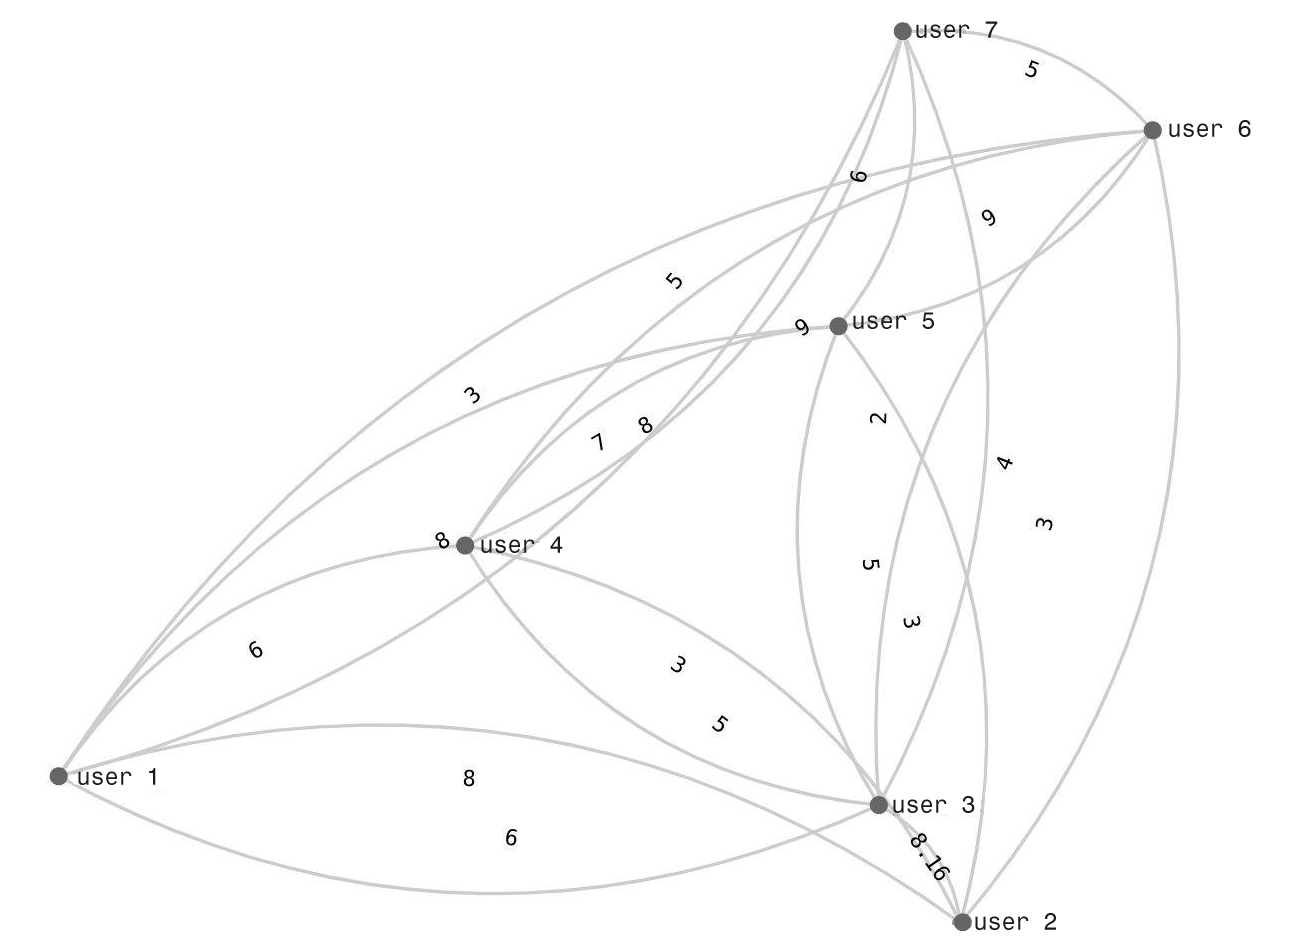
\includegraphics[width=12cm]{grafo.png}
\caption{Um grafo com 5 nós e 6 arestas.}
\label{fig:grafo}
\end{figure}

Quando a relação entre dois nós é simétrica, ou seja, a relação entre o nó $A$ e o nó $B$ é idêntica, diz-se que o grafo é \emph{não orientado}. Quando a relação entre dois nós é assimétrica, portanto, $A$ tem uma relação com $B$, mas essa relação não equivale a $B$ para $A$, tem-se um \emph{dígrafo} ou um \emph{grafo orientado}.

Este trabalho utiliza o grafo não orientado pois este bem representa as relações de amizade recíprocas. Tal decisão é tomada pois, quando da sugestão de um novo contato, ambos vão ser apresentados reciprocamente, estabelecendo, portanto, uma relação mútua de interação.

Diversas áreas da ciência, desde a biologia à linguística, utilizam grafos para representar dados. A representação de objetos e suas relações é uma ferramenta frequente em várias pesquisas.

Na ciência da computação, o grafo é a uma estrutura de dados amplamente frequente e existem centenas de problemas computacionais definidos com o seu uso \cite{Cormen2009}. Um caso tradicional com solução utilizando grafos é a do caixeiro viajante. Neste problema, os nós do grafo são as localidades e as arestas têm o peso equivalente à distância entre as cidades. \citep{Dijkstra1959}, propôs o primeiro algoritmo para encontrar o caminho mais curto entre dois nós de um grafo. O algoritmo encontra um caminho curto, mas não necessariamente o mais curto. Vários trabalhos são realizados ainda hoje na busca pelo caminho mais curto em um grafo. Muitos desses trabalhos são baseados no algoritmo de Dijkstra.

Como estrutura de dados computacionais, existem várias modelagens conhecidas para representação de um grafo. \citep{Cormen2009}, cita duas formas fundamentais:

\begin{itemize}
\item A lista de adjacência
\item A matriz de adjacência
\end{itemize}

\begin{figure}[!htb]
\centering
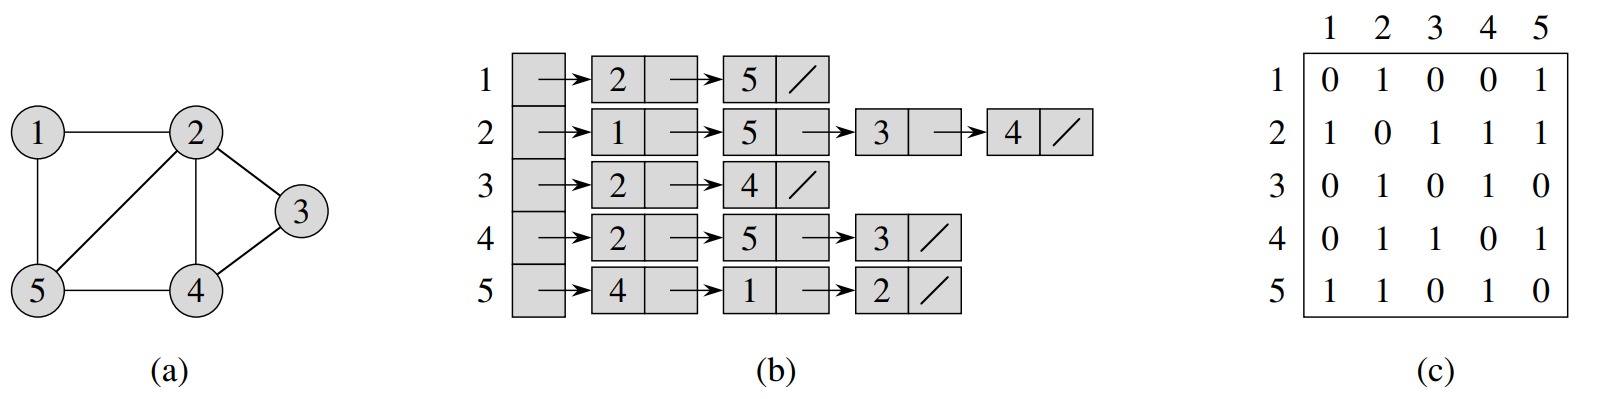
\includegraphics[width=16cm]{represent_grafo.png}
\caption{Duas representações de um grafo não direcionado. (\textbf{a}) Um grafo G com cinco nós e sete arestas. (\textbf{b}) A representação de uma lista de adjacência de G. (\textbf{c}) A representação de uma matriz de adjacência. Fonte: \cite{Cormen2009}, tradução dos autores.}
\label{fig:represent_grafo}
\end{figure}


\begin{figure}[!htb]
\centering
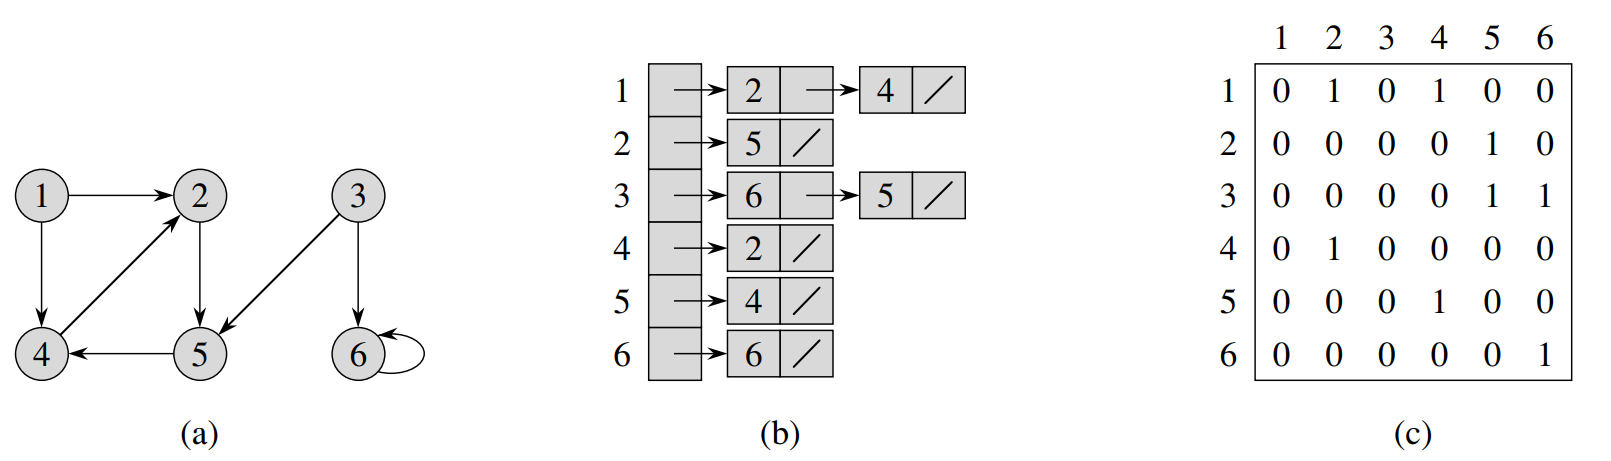
\includegraphics[width=16cm]{represent_grafo_ND.png}
\caption{Duas representações de um grafo direcionado. (\textbf{a}) Um grafo G com seis nós e oito arestas. (\textbf{b}) A representação de uma lista de adjacência de G. (\textbf{c}) A representação de uma matriz de adjacência. Fonte: \cite{Cormen2009}, tradução dos autores.}
\label{fig:represent_grafo_ND}
\end{figure}

\FloatBarrier

A Figura \ref{fig:represent_grafo}, ilustra um grafo $G$ como um diagrama, como uma lista de adjacência e como uma matriz de adjacência. A implementação computacional de um grafo pode ser a partir de uma lista de adjacência. Desse modo Um grafo $G = (N, E)$ consiste de uma lista de listas de nós, uma lista para cada nó em N. Para cada nó em G, tem-se uma lista dos nós vizinhos. Essa lista também pode conter somente um ponteiro para os nós vizinhos. Normalmente é suficiente armazenar os nós vizinhos em ordem arbitrária pois será o peso da aresta que determinará uma hierarquia entre os nós vizinhos, não a ordem pela qual eles foram adicionados nem qualquer outro atributo.


% inclusão de apêndice
\chapter{Fundamentação Teórica}
\label{cap:fund}

% figuras estão no subdiretório "figuras/" dentro deste capítulo
\graphicspath{\currfiledir/figuras/}

Nesta parte, há a exposição das definições e histórico de redes sociais, algoritmos de recomendação e as definições matemáticas e computacionais de grafo. Esses três itens relacionam-se intrinsicamente com este trabalho, por isso, buscamos esclarecê-los o suficiente neste capítulo de maneira que as relações destes tópicos com o objetivo geral estejam fundamentadas.


\section{Redes Sociais}

% \begin{itemize}
% \item Histórico de redes sociais
% \item Tipos de redes sociais
% \item Redes parecidas com nosso trabalho
% \item Análises de tempo despendido em redes sociais.
% \end{itemize}

Desde a invenção da internet em 1991, mais e mais aplicações vem sendo criadas para facilitar e estimular os relacionamentos virtuais. As redes sociais virtuais tiveram início em 1997 com o site \emph{Six Degrees}, \citep{terrel17}. \emph{Six Degrees} é nomeado em referência ao estudo de \cite{milgram67}, que teorizava que são necessários seis laços de amizade para que quaisquer pessoas estejam conectadas. \emph{Six Degrees} teve seu fim em 2001, mas iniciou o processo de popularização das redes sociais e é considerado a primeira rede social pois permitia que as pessoas criassem seus perfis individuais e adicionar outros contatos à sua rede. Teve 3,5 milhões de usuários no seu auge.

Entre as precursoras está também a rede especializada em relacionamentos profissionais, \emph{LinkedIn}. Foi criada no final de 2002 e tem, desde então, seu objetivo principal em criar conexões entre profissionais, estudantes e corporações. O \emph{LinkedIn} é, ainda hoje, a rede mais popular neste nicho com mais de 500 milhões de usuários.

A rede mais popular atualmente, segundo \cite{lua19}, é o Facebook com 2,23 milhões de usuários ativos mensalmente. O Facebook foi criado em 2004 como uma rede específica para estudantes da Universidade de Harvard. Em 2006 foi aberta ao público e em 2008 já era a rede social mais visitada do mundo.

Há também redes especializadas em outros tipos de conexão ou outras maneiras de publicar conteúdo. O YouTube é uma rede social especializada na divulgação de vídeos criados pelos usuários. O Twitter, distingue-se das outras redes por iniciar suas atividades permitindo apenas a publicação de textos com, no máximo, 140 caracteres. Este limite foi dobrado posteriormente, mas o foco ainda mantém-se em pequenas postagens.

Por fim, há as redes especializadas em relacionamentos românticos. O Tinder, o Happn e o OKCupid são exemplos de redes sociais direcionadas à criação de relacionamentos íntimos entre os usuários. O sistema desenvolvido neste trabalho enquadra-se nesta categoria pois tem o objetivo de colocar usuários em contato com pessoas desconhecidas que têm potencial para formarem amizades ou até mesmo casais.

No Brasil, 66\% da população tem acesso à internet segundo \cite{wearesocial18}. Dentre os usuários da internet 93\% são ativos em alguma rede social.
Segundo \cite{wearesocial18}, o brasileiro despende, em média, 3h39min por dia em alguma rede social. Este tempo é passado em contato com informações e pessoas de várias culturas diferentes. Muitas vezes as interações despertam sentimentos indesejados e a informação divulgada não é completamente conexa à realidade.

Por essa razão, mais e mais redes sociais oferecem a oportunidade, muitas vezes compulsoriamente, do usuário ser exposto somente à pessoas e conteúdos que tenham afinidade com seu perfil. Na busca por uma experiência agradável, as sugestões de conteúdo e contatos vão ao encontro da necessidade do ser humano de se socializar. E participar de uma rede social, seja ela física ou virtual, faz parte das necessidades básicas apontadas por \cite{Maslow1943}, ao definir uma hierarquia para as necessidades básicas do ser humano.

De uma maneira ou de outra, todas as redes sociais tem seu foco no conteúdo gerado pelos usuários. Porém, grande parte da monetização empregada refere-se à divulgação de peças publicitárias pagas por empresas particulares e públicas. Dentro deste escopo, são utilizados algoritmos que tomam em conta os interesses dos usuários para fazer sugestões de conteúdo publicitário. Há vários métodos para relacionar os dados produzidos pelos usuários para gerar sugestões, sejam elas de conteúdo, publicidade ou novos contatos.

%=====================================================

\section{Algoritmos de Recomendação}

% \begin{itemize}
% \item Como sugerir novos contatos.
% \item Como as outras redes fazem isso.
% 
% \end{itemize}


Quando um usuário acessa um sistema qualquer que lhe oferece itens, por exemplo, livros, um sistema de recomendação pode lhe proporcionar a conveniência de sugerir-lhe um livro mais adequado para o seu gosto quando a quantidade de opções disponíveis é opressivamente vasta, diz \cite{Ricci2010}.

Esses itens, são quaisquer coisas que podem ser sugeridas ao usuário, sejam produtos, serviços, notícias, publicidade, ou, no caso deste trabalho, outros usuários com potencial para tornarem-se amizades.

Para \cite{Ricci2010}, a forma mais simples de um sistema de recomendação é uma lista com itens ordenados pela similaridade com o usuário que receberá a recomendação. Os sistemas de sugestão analisam vários tipos de dados por diversos métodos diferentes para encontrar os itens mais adequados para cada usuário. De acordo com \cite{Ricci2010}, os primeiros algoritmos de recomendação utilizavam dados gerados por recomendações feitas pela comunidade de usuários. Esse método comparava gostos similares entre os usuários e recomendava itens ainda não consumidos por alguns usuários. A este método dá-se o nome de Filtragem Colaborativa \citep{goldberg92}.

Desde os anos 1990, a perseguição por sistemas de recomendações cada vez mais eficientes impulsionou o surgimento do Prêmio Netflix em 2006, \citep{netflix}. Neste concurso, a empresa Netflix propôs pagar um prêmio de US\$1.000.000 para quem elaborasse um sistema que pudesse melhorar em, pelo menos, 10\% a acurácia do sistema que estava em uso à época. O time \emph{BellKor's Pragmatic Chaos}, venceu a disputa empregando diversos algoritmos e métodos de classificação mesclados em um mesmo sistema, \citep{Bell}. 

Entre as possibilidades de métodos e algoritmos que podem ser empregados em um sistema de recomendação, podemos ressaltar, baseados no texto de \cite{Recommendation}, as seguintes:

\begin{itemize}
\item Filtragem colaborativa
\item Filtragem baseada em conteúdo
\item Recomendação baseada em conhecimento
\end{itemize}

A filtragem colaborativa, como já mencionado, leva em conta as preferências já informadas pelos usuários para compará-las e sugerir novas possibilidades de itens. Tem a tendência de sugerir itens que já são apreciados por usuários que, de alguma maneira, já se relacionam, seja por interesses definidos, grupos específicos ou até mesmo por parentesco.

A filtragem baseada em conteúdo toma por verdadeira a afirmação de que os usuários que já demonstraram interesse por um tópico somente serão agradados por tópicos semelhantes e não podem ser instigados por assuntos fora do escopo do que já foi definido como interesse inicialmente. Dessa maneira, o sistema considera de que um usuário que declarou interesse por filmes deve receber sugestões de itens relacionados a este tema. É claro que este método tem a fraqueza de não sugerir novos assuntos que, potencialmente, despertariam o interesse do usuário.

Finalmente, a recomendação baseada em conhecimento,  que toma em conta regras de restrições de interesse definidas no sistema e os aplica à lista de itens disponíveis. Desse modo, os itens são sugeridos a partir do resultado da filtragem realizada a partir das regras definidas. A definição de tais regras passa por análises semânticas do conteúdo disponível no sistema que diga respeito ao usuário. O sistema desenvolvido neste trabalho assemelha-se a uma recomendação baseada em conhecimento no sentido de que a regra definida para relacionar os itens será uma equação determinística que calcula um valor de proximidade entre dois itens.

Os vários métodos de recomendação tem sua acurácia diretamente influenciada pela quantidade de informação disponível sobre os usuários ou gerada pelos usuários. Quanto maior a quantidade de informação disponível, maior a acurácia e, em linhas gerais, menor a performance do sistema, uma vez que o tempo de processamento da informação é incrementado. Por essa razão, boas soluções são baseadas em aprendizado de máquina e inteligência artificial. O emprego dessas tecnologias tem o objetivo de melhorar a performance e a acurácia das sugestões.

%=====================================================

\section{Grafo}
% \begin{itemize}
% \item O que é grafo - \emph{Fonte básica de definição de grafo LIVRO??}
% \item Quantos tipos de grafo existem.
% \item Aplicações comuns de grafo
% \item Algoritmos que usam grafos
% \end{itemize}

O conceito matemático de grafo parte de abstrações de situações da vida real onde objetos ou pessoas representadas por pontos e suas conexões e interações são representadas por linhas \cite{Bondy08}. Numa rede social, as pessoas são esses pontos, que convencionalmente são chamados de nós, e suas relações com outras pessoas são representadas por linhas, chamadas de arestas. Um grafo é uma tripla ordenada $G=(N(G), A(G), \psi _{G})$, que consiste de um conjunto não vazio $N(G)$ de nós, um conjunto $A(G)$, diferente de $N(G)$, de arestas, e uma \emph{função de incidência} $\psi_{G}$ que associa a cada nó de $G$ um par não ordenado de nós de $G$. Se $e$ é uma aresta de $G$ e $u$ e $v$ são arestas de tal modo que $\psi_{G}(e) = un$, então $e$ é dito que \emph{une} $u$ e $n$ \cite{Bondy08}.

\emph{Exemplo}

\begin{equation}
G=(N(G), A(G), \psi _{G})
\label{eq:grafo}
\end{equation}

\emph{onde}

\begin{equation}
N(G)={n_{1}, n_{2}, n_{3}, n_{4}, n_{5}}
\label{eq:grafo2}
\end{equation}

\emph{e $\psi_{G}$ é definido por}

\begin{equation}
\begin{split}
\psi_{G}(a_{1}) = n_{1}n_{2}, \psi_{G}(a_{2} = n_{2}n_{3}, \psi_{G}(a_{3}) = n_{3}n_{3}, \psi_{G}(a_{4}) = n_{2}n_{4} \\
\psi_{G}(a_{5}) = n_{2}n_{4}, \psi_{G}(a_{6} = n_{4}n_{5}, \psi_{G}(n_{8}) = n_{2}n_{5}, \psi_{G}(a_{4}) = n_{2}n_{4}
\label{eq:grafo3}
\end{split}
\end{equation}

Grafos têm este nome pois podem ser representadas graficamente, segundo \cite{Bondy08}. A Figura \ref{fig:grafo}, é um diagrama que representa um grafo com 5 nós e 6 arestas. Nesta Figura, os nós têm identificação - letras - e as arestas tem um \emph{peso}. O peso das arestas pode ser usado para representar a força da ligação entre os nós ou até mesmo a distância entre os nós. A convenção tomada neste caso depende do contexto e da aplicação do grafo.

\begin{figure}[!htb]
\centering
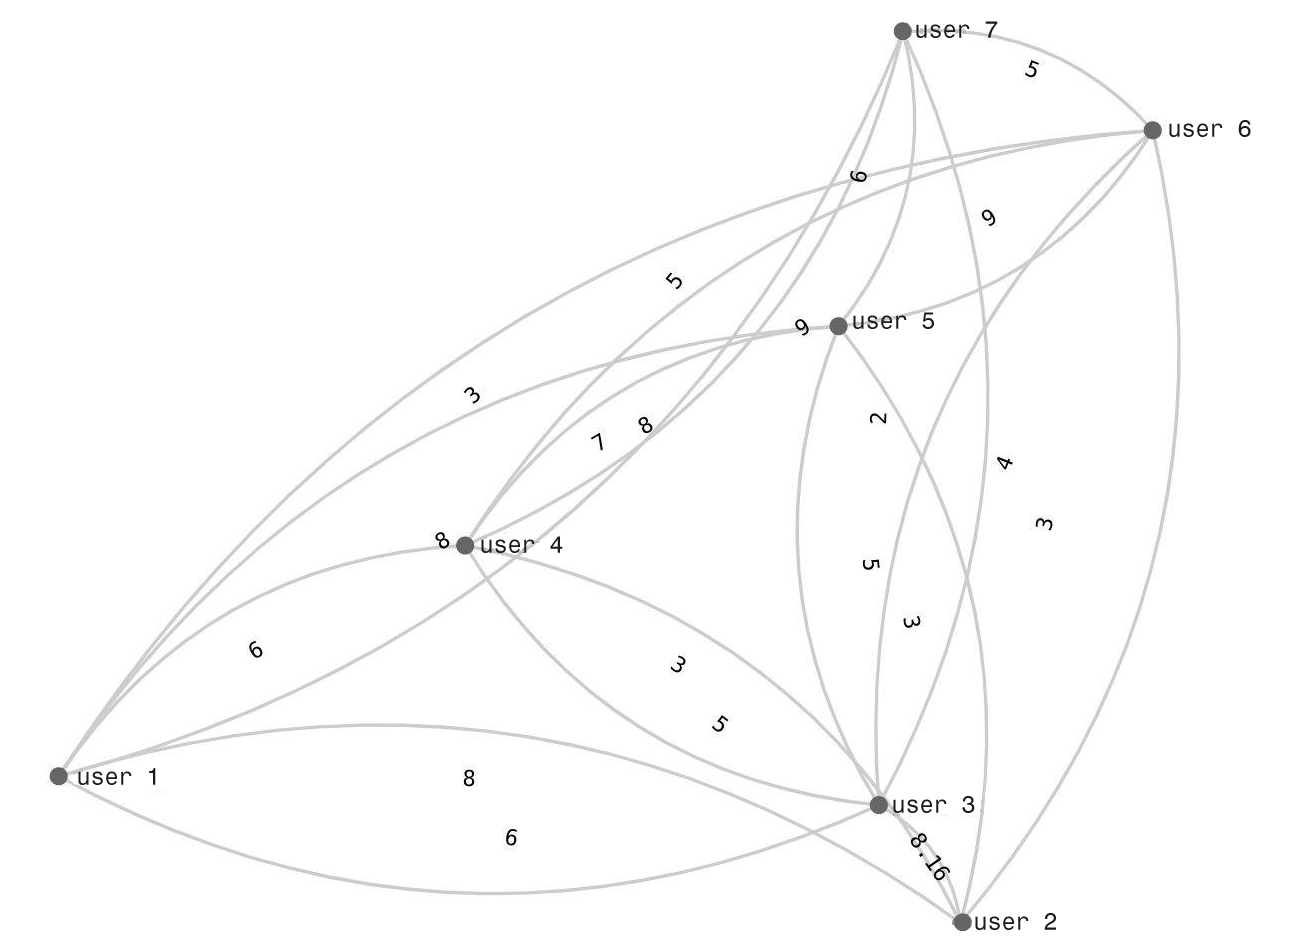
\includegraphics[width=12cm]{grafo.png}
\caption{Um grafo com 5 nós e 6 arestas.}
\label{fig:grafo}
\end{figure}

Quando a relação entre dois nós é simétrica, ou seja, a relação entre o nó $A$ e o nó $B$ é idêntica, diz-se que o grafo é \emph{não orientado}. Quando a relação entre dois nós é assimétrica, portanto, $A$ tem uma relação com $B$, mas essa relação não equivale a $B$ para $A$, tem-se um \emph{dígrafo} ou um \emph{grafo orientado}.

Este trabalho utiliza o grafo não orientado pois este bem representa as relações de amizade recíprocas. Tal decisão é tomada pois, quando da sugestão de um novo contato, ambos vão ser apresentados reciprocamente, estabelecendo, portanto, uma relação mútua de interação.

Diversas áreas da ciência, desde a biologia à linguística, utilizam grafos para representar dados. A representação de objetos e suas relações é uma ferramenta frequente em várias pesquisas.

Na ciência da computação, o grafo é a uma estrutura de dados amplamente frequente e existem centenas de problemas computacionais definidos com o seu uso \cite{Cormen2009}. Um caso tradicional com solução utilizando grafos é a do caixeiro viajante. Neste problema, os nós do grafo são as localidades e as arestas têm o peso equivalente à distância entre as cidades. \citep{Dijkstra1959}, propôs o primeiro algoritmo para encontrar o caminho mais curto entre dois nós de um grafo. O algoritmo encontra um caminho curto, mas não necessariamente o mais curto. Vários trabalhos são realizados ainda hoje na busca pelo caminho mais curto em um grafo. Muitos desses trabalhos são baseados no algoritmo de Dijkstra.

Como estrutura de dados computacionais, existem várias modelagens conhecidas para representação de um grafo. \citep{Cormen2009}, cita duas formas fundamentais:

\begin{itemize}
\item A lista de adjacência
\item A matriz de adjacência
\end{itemize}

\begin{figure}[!htb]
\centering
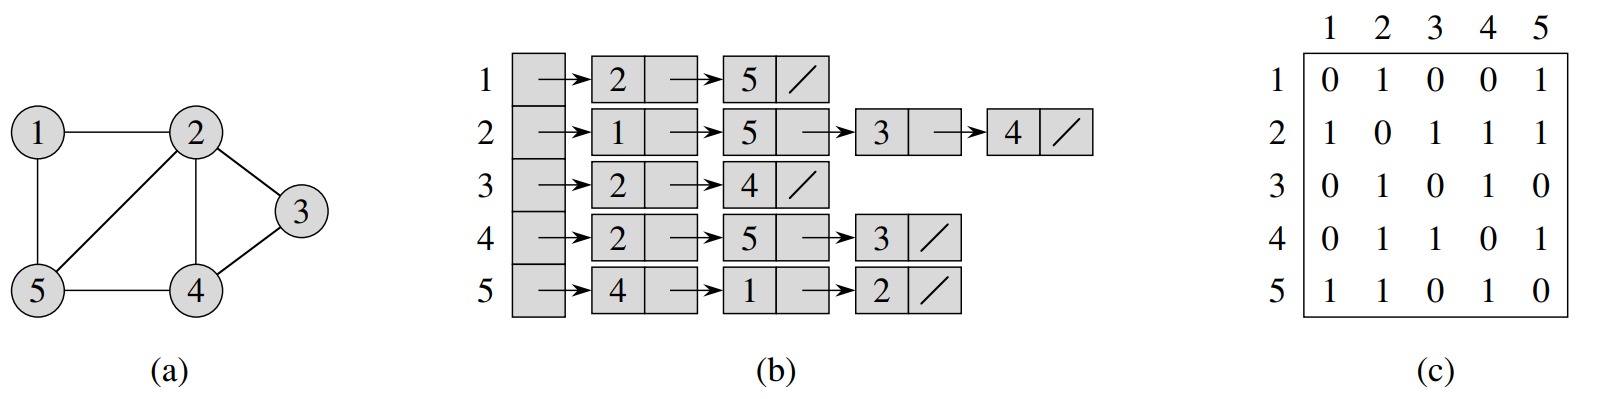
\includegraphics[width=16cm]{represent_grafo.png}
\caption{Duas representações de um grafo não direcionado. (\textbf{a}) Um grafo G com cinco nós e sete arestas. (\textbf{b}) A representação de uma lista de adjacência de G. (\textbf{c}) A representação de uma matriz de adjacência. Fonte: \cite{Cormen2009}, tradução dos autores.}
\label{fig:represent_grafo}
\end{figure}


\begin{figure}[!htb]
\centering
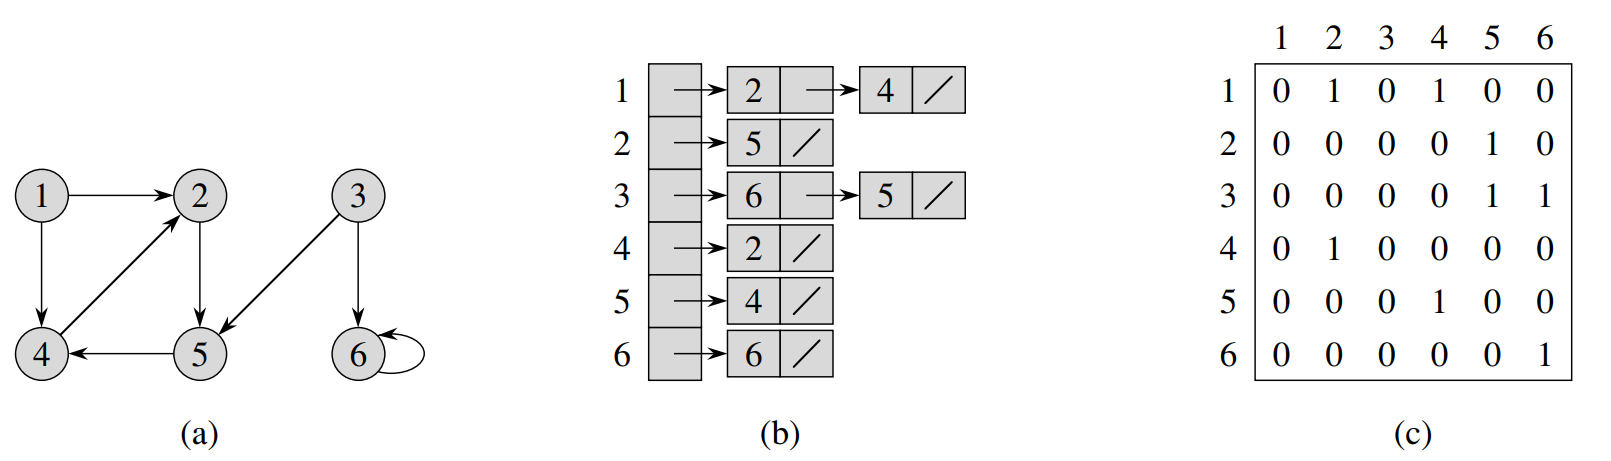
\includegraphics[width=16cm]{represent_grafo_ND.png}
\caption{Duas representações de um grafo direcionado. (\textbf{a}) Um grafo G com seis nós e oito arestas. (\textbf{b}) A representação de uma lista de adjacência de G. (\textbf{c}) A representação de uma matriz de adjacência. Fonte: \cite{Cormen2009}, tradução dos autores.}
\label{fig:represent_grafo_ND}
\end{figure}

\FloatBarrier

A Figura \ref{fig:represent_grafo}, ilustra um grafo $G$ como um diagrama, como uma lista de adjacência e como uma matriz de adjacência. A implementação computacional de um grafo pode ser a partir de uma lista de adjacência. Desse modo Um grafo $G = (N, E)$ consiste de uma lista de listas de nós, uma lista para cada nó em N. Para cada nó em G, tem-se uma lista dos nós vizinhos. Essa lista também pode conter somente um ponteiro para os nós vizinhos. Normalmente é suficiente armazenar os nós vizinhos em ordem arbitrária pois será o peso da aresta que determinará uma hierarquia entre os nós vizinhos, não a ordem pela qual eles foram adicionados nem qualquer outro atributo.


%=====================================================

\end{document}

%=====================================================
